	%After first compiling run following commands in command prompt and compile again:
%bibtex Proposal - where Proposal is the name of your main file
%makeglossaries Proposal - where Proposal is the name of your main file

%\documentclass[twoside, openright, a4paper,12pt]{report} % Two side 
\documentclass[oneside,a4paper,12pt]{book} 

\setcounter{secnumdepth}{3}

\usepackage{pdfpages}
\usepackage{JMTemplate}
\usepackage{tikz}
\usetikzlibrary{automata,positioning}
\usepackage{amsthm}
\usepackage{amssymb}
\usepackage[]{amsmath}
\usepackage{caption}
\usepackage{subcaption}
\usepackage{dsfont}
\usepackage{array}
\usepackage{pgfplots}
\usepackage{color}

\definecolor{darkgreen}{RGB}{47,109,79}
\definecolor{darkblue}{RGB}{57,79,99}
\definecolor{rosso}{RGB}{220,57,18}
\definecolor{giallo}{RGB}{255,153,0}
\definecolor{blu}{RGB}{102,140,217}
\definecolor{verde}{RGB}{16,150,24}
\definecolor{viola}{RGB}{153,0,153}
\definecolor{awesome}{rgb}{1.0, 0.13, 0.32}
\definecolor{ref}{rgb}{0.65,0.65,0.65} %{0.4,0.8,0.85}
\definecolor{highlightrow}{rgb}{0.9,0.9,0.9}

\newcommand{\norm}[1]{\left\lVert#1\right\rVert}
\newcommand*{\prob}{\mathbb P}
\newcommand*{\expected}{\mathbb E}
\newcommand{\bff}[1]{{\bf #1}}
\newcommand{\bb}[1]{{\mathbb{#1}}}
\newcommand{\bbm}[1]{{\mathbbm{#1}}}
\newcommand{\mcal}[1]{{\mathcal{#1}}}

\newcommand{\task}{وظیفه‌}
\newcommand{\beamsearch}{جست و جوی پرتویی}
\newcommand{\likelihood}{درست‌نمایی}
\newcommand{\mle}{بیشینه درست‌نمایی}
\newcommand{\teacherforcing}{جبر معلم}
\newcommand{\pretrain}{پیش‌آموزش}
\newcommand{\maxlikelihood}{بیشینه درست‌نمایی}
\newcommand{\noise}{نوفه}
\newcommand{\argmaxphrase}{آرگومان بیشینه یابی}
\newcommand{\augmentation}{افزودن داده}

\newcommand{\transportplan}{طرح جابه‌جایی}
\newcommand{\earthmover}{\lr{Earth-Mover}}
\newcommand{\lipschitz}[1][]{\lr{#1Lipschitz}}

\newcommand{\vae}{خودکدنگار وردشی}
\newcommand{\cvae}{خودکدنگار وردشی شرطی}
\newcommand{\towardctg}{\lr{CTG}}
\newcommand{\reparametrization}{پارامتری‌سازی مجدد}
\newcommand{\priordist}{توزیع پیشین}
\newcommand{\posterior}{پسین}
\newcommand{\posteriordist}{توزیع پسین}
\newcommand{\encoder}{کدگذار}
\newcommand{\decoder}{کدگشا}
\newcommand{\inference}{استنتاج}
\newcommand{\latentvar}{متغیر نهان}

\newcommand{\gan}{شبکه‌های تخاصمی مولد}
\newcommand{\cgan}{شبکه‌ تخاصمی مولد شرطی}
\newcommand{\sentigan}{\lr{SentiGAN}}
\newcommand{\reinforce}{یادگیری تقویتی}
\newcommand{\policygradient}{گرادیان تابع سیاست}
\newcommand{\transitionfunc}{تابع گذار}
\newcommand{\rewardfunc}{تابع پاداش}
\newcommand{\deterministic}{قطعی}
\newcommand{\generative}{مولد}
\newcommand{\classifier}{دسته‌بند}
\newcommand{\discriminator}{تمییزدهنده}
\newcommand{\montecarlotreesearch}{جست‌وجوی مونت کارلو درختی}
\newcommand{\montecarlosearch}{جست‌وجوی مونت کارلو}
\newcommand{\generator}{مولد}
\newcommand{\minmaxgame}{بازی بیشینه/کمینه}
\newcommand{\modecollapse}{چسبیدگی به قله}
\newcommand{\meanseeking}{میانگین جویانه}
\newcommand{\critic}{نقاد}

\newcommand{\aae}{خودکدنگار تخاصمی}
\newcommand{\marginal}{حاشیه‌ای}
\newcommand{\uniaprox}{تخمین گر عمومی}

\newcommand{\wae}{خودکدنگار واسرشتاین}
\newcommand{\wgan}{شبکه‌های تخاصمی مولد واسرشتاین}
\newcommand{\wasser}{واسرشتاین}
\newcommand{\mmd}{\lr{MMD}}
\newcommand{\reproducing}{با قابلیت بازتولید}
\newcommand{\ancestral}{سلسله مراتبی}
\newcommand{\dilated}{انبساطی}
\newcommand{\receiptivefield}{حوزه تاثیر}
\newcommand{\bitsback}{\lr{Bits-Back}}

\newcommand{\autoencoder}{خودکدنگار}
\newcommand{\condtg}{تولید متن به صورت شرطی}
\newcommand{\symbolic}{نمادین}
\newcommand{\recall}{فراخوانی}
\newcommand{\autoregressive}{خود برگشتی}
\newcommand{\expbias}{اریبی مواجهه}
\newcommand{\sgd}{گرادیان کاهشی تصادفی}
\newcommand{\localopt}{بهینه محلی}
\newcommand{\semisupervised}{نیمه‌نظارتی}
\newcommand{\unsupervised}{بدون نظارت}
\newcommand{\jointlabeled}{جفت برچسب زده شده}
\newcommand{\paraphrase}{بازعبارت‌بندی}
\newcommand{\embedding}{تعبیه}
\newcommand{\baseline}{مدل پایه}
\newcommand{\conditional}{شرطی}
\newcommand{\representation}{بازنمایی}

\newcommand{\flow}{جریان}
\newcommand{\normalizingflownets}{شبکه‌های مبتنی بر جریان نرمال‌کننده}
\newcommand{\normalizingflownet}{شبکه مبتنی بر جریان نرمال‌کننده}
\newcommand{\elementwise}{درایه‌گرا}
\newcommand{\coupling}{اتصالی}
\newcommand{\conditioner}{شرطی‌کننده}
\newcommand{\blocktrimatrix}{ماتریس مثلثی بلوکی}
\newcommand{\gpu}{واحد پردازش‌گر گرافیک}
\newcommand{\univapprox}{تخمین‌گر عمومی}
\newcommand{\affine}{هم‌نسبی}
\newcommand{\gaussianmix}{مخلوط گاوسی}
\newcommand{\crossentropy}{\lr{Cross-Entory}}
\newcommand{\simplex}{سادک}
\newcommand{\onehot}{تک یک}
\newcommand{\forward}{پیش‌رو}
\newcommand{\backward}{پس‌رو}
\newcommand{\spline}{اسپلاین}

\newcommand{\bleu}[1][]{\lr{BLEU#1}}
\newcommand{\selfbleu}[1][]{\lr{Self-BLEU#1}}
\newcommand{\perplexity}{\lr{Perplexity}}
\newcommand{\revperplexity}{\lr{Reverse Perplexity}}
\newcommand{\jaccard}[1][]{\lr{MS-Jaccard#1}}
\newcommand{\greedydecoding}{کدگشایی حریصانه}
\newcommand{\validation}{اعتبارسنجی}
\newcommand{\decode}{کدگشایی}
\newcommand{\encode}{کدگذاری}
\newcommand{\lstm}{شبکه‌های با حافظه کوتاه مدت ماندگار}
\newcommand{\cnn}{شبکه‌های عصبی پیچشی}
\newcommand{\rnn}{شبکه عصبی خودبازگشتی}

\newcommand{\transformer}{\lr{Transformer}}
\newcommand{\stateoftheart}{لبه تکنولوژی}
\newcommand{\seqtoseq}{دنباله به دنباله}
\newcommand{\multiheadselfattention}{خودتوجه چند سر}
\newcommand{\multiheadattention}{توجه چند سر}
\newcommand{\feedfoward}{پیش‌خور}
\newcommand{\fullyconnected}{تمام متصل}
\newcommand{\residual}{باقی‌مانده}
\newcommand{\layernormalization}{نرمال‌کننده لایه}
\newcommand{\query}{پرسمان}
\newcommand{\keyvaluepair}{جفت کلید-مقدار}
\newcommand{\dotattention}{توجه با استفاده از ضرب داخلی مقیاس شده}
\newcommand{\softmax}{\lr{Softmax}}
\newcommand{\mask}{نقاب}
\newcommand{\positionalembedding}{تعبیه مکانی}
\newcommand{\recurrence}{بازگشتی}
\newcommand{\encoding}{کدگذاری}

\newcommand{\ngramphrase}{\rl{n}-گرام‌}
\newcommand{\correlation}{همبستگی}
\newcommand{\finetuning}{به‌آموزی}
\newcommand{\huristic}{اکتشافی}

\newcommand{\sst}{\lr{SST}}
\newcommand{\yelp}{\lr{Yelp}}
\newcommand{\amazon}{\lr{Amazon}}
% Information for pdf making 
%=======================================================
\newcommand{\fatype}{پایان‌نامه}
\newcommand{\fatitle}{
طراحی یک سامانه‌ی مکالمه دامنه‌باز مبتنی بر دانش
}
\newcommand{\faAuthor}{محمدمهدی سمیعی پاقلعه}
\newcommand{\fasupervisor}{دکتر حسین صامتی}
\newcommand{\fahamkar}{- - -}
\newcommand{\famoshaver}{- - -}
\newcommand{\fadate}{تابستان ۱۳۹۹}
\newcommand{\famajor}{گرایش هوش مصنوعی}
\newcommand{\falevel}{کارشناسی ارشد}
\newcommand{\fadepart}{دانشکده مهندسی کامپیوتر}

\newcommand{\entype}{Thesis}
\newcommand{\entitle}{Design of a knowledge-grounded open domain dialogue system }
\newcommand{\enAuthor}{Mohammad Mahdi Samiei Paqaleh}
\newcommand{\ensupervisor}{Dr. H. Sameti}
\newcommand{\engdate}{Summer 2020}
\newcommand{\enmajor}{Artificial Intelligence}
\newcommand{\enlevel}{M.Sc.}
\newcommand{\enDep}{Department of Computer Engineering}

\newcommand{\momtaheninFirst}{دکتر حمید بیگی}
\newcommand{\momtahenouFirst}{دکتر داور خارجی}



\hypersetup{
   pdftitle={\entitle} 
   ,pdfauthor ={\enAuthor}
   ,pdfsubject={\enlevel{} \entype{} (\enmajor), \enDep, Sharif University of Technology, Tehran, Iran}
}

\glsdisablehyper % disable hyperlinks

\newglossarystyle{persian-to-english}{%
%	\glossarystyle{listdotted}% the base style
	% put the glossary in a two column page and description (as in listdotted style) environment:
	\renewenvironment{theglossary}%
		{\begin{multicols}{2}\begingroup \flushleft }%
		{\endgroup \end{multicols}}%
%	\renewenvironment{theglossary}{}{}%
	% have nothing after \begin{theglossary}:
	\renewcommand*{\glossaryheader}{}%
	% have nothing between glossary groups:
	\renewcommand*{\glsgroupheading}[1]{}%
	\renewcommand*{\glsgroupskip}{}%
	% set how each entry should appear: \glossaryentryfield{label}{formatted name}{description}{symbol}{number list}
	\renewcommand*{\glossaryentryfield}[5]{%
		\glstarget{##1}{##2}% persian term
		\dotfill%dots
		\space \lr{##3} \\%
%		\dotfill%
%		\space {##5} \\%translation term
	}%
	% set how sub-entries appear:
	\renewcommand*{\glossarysubentryfield}[6]{%
		\glossaryentryfield{##2}{##3}{##4}{##5}{##6}%
	}%
}
% ========= Glossary styles (put in files) =========
\newglossarystyle{english-to-persian}{%
%	\glossarystyle{listdotted}% the base style
	% put the glossary in a two column page and description (as in listdotted style) environment:
	\renewenvironment{theglossary}%
		{\begin{multicols}{2}\begingroup \flushright }%
		{\endgroup \end{multicols}}%
%	\renewenvironment{theglossary}{\Latin{}}{\Persian{}}%
	% have nothing after \begin{theglossary}:
	\renewcommand*{\glossaryheader}{}%
	% have nothing between glossary groups:
	\renewcommand*{\glsgroupheading}[1]{}%
	\renewcommand*{\glsgroupskip}{}%
	% set how each entry should appear:
	\renewcommand*{\glossaryentryfield}[5]{%
		\glstarget{##1}{##2}% persian term
		\dotfill%dots
		\space \rl{##3} \\%translation term
	}%
	% set how sub-entries appear:
	\renewcommand*{\glossarysubentryfield}[6]{%
		\glossaryentryfield{##2}{##3}{##4}{##5}{##6}%
	}%
}

% ========= GLOSSARIES =========
\newglossary{p2e-terms}{fa.gls}{fa.glo}{واژه‌نامه فارسی به انگلیسی} % persian to english
\newglossary{e2p-terms}{en.gls}{en.glo}{English to Persian Glossary} % english to persian

\newcommand{\newtrans}[3][]{% params: persian, english translations, first optional is a key
\newtranspl[#1]{#2}{#3}{#2‌ها}%
}

\newcommand{\newtranspl}[4][]{% params: persian, english, plural form of persian, first optional is a key
\ifthenelse{\isempty{#1}}{\def\key{#2}}{\def\key{#1}}%
\newglossaryentry{en:\key}{type={e2p-terms}, name={#3}, description={#2}}% english glossary
%	\newglossaryentry{fa:\key}{type={p2e-terms}, name={#2}, description={#3}}% persian glossary
\newglossaryentry{fa:\key}{type={p2e-terms}, name={#2}, plural={#4}, description={#3}}% persian glossary
}
% ========= END OF GLOSSARIES =========

% Show a translation and footnote it.
% Params (the same as \glsdisplayfirst):{text}{description}{symbol}{insert}
% insert can possibly be filled with some notes on the translation.
\newcommand{\showTransFirst}[4]{%  translation for the first time
\ifthenelse{\isempty{#4}}%
{\textit{#1}\LTRfootnote{ #2}}% if #4 is empty (no notes) 
%%%{\textit{#1}\LTRfootnote{{#2} #4}}% if #4 is not empty
{\textiranic{#1}\LTRfootnote{{#2} #4}}% if #4 is not empty
%{\textit{#1}\footnote{ \lr{#2}؛  #4}}% if #4 is not empty
}

\newcommand{\showTrans}[4]{% translation for next times
\ifthenelse{\isempty{#4}}%
{{#1}}% if #4 is empty (no notes) 
{\textit{#1}\footnote{#4}}% if #4 is not empty
}

\defglsdisplayfirst[p2e-terms]{\showTransFirst{#1}{#2}{#3}{#4}}% protect fragile commands
\defglsdisplay[p2e-terms]{\showTrans{#1}{#2}{#3}{#4}}

% Symbol may temporarily used to keep some notes on the translation.
% It must be replaced with a user1 key which now raises error, texlive must be upgraded.
\newcommand{\term}[2][]{%
\glsadd{en:#2}%
\ifthenelse{\isempty{#1}}{\gls{fa:#2}}{\gls{fa:#2}[#1]}%
}
\newcommand{\termpl}[2][]{%
\glsadd{en:#2}%
\ifthenelse{\isempty{#1}}{\glspl{fa:#2}}{\glspl{fa:#2}[#1]}%
}
%=========== Print Glossaries ===============
% see: http://www.parsilatex.com/forum/SMF/index.php?topic=345.0
%\glossarystyle{persian-to-english}
%\def\glossaryname{واژه‌نامه فارسی به انگلیسی}
%\printglossaries

\newcommand{\printpersianglossary}[1][واژه‌نامه فارسی به انگلیسی]{{%
	\phantomsection % hyperref: enable hyperlinking from the table of contents to this point
	\addcontentsline{toc}{chapter}{#1} % add a line in the Table of Contents (first option, toc), it will be like the ones 
	\renewcommand{\glossarymark}[1]{\markboth{##1}}% correct handling of page header
	\printglossary[type={p2e-terms},style={persian-to-english},title={#1}]%
}}


\newcommand{\printenglishglossary}[1][واژه‌نامه انگلیسی به فارسی]{{%
	\phantomsection % hyperref: enable hyperlinking from the table of contents to this point
	\addcontentsline{toc}{chapter}{#1} % add a line in the Table of Contents (first option, toc), it will be like the ones 
	\renewcommand{\glossarymark}[1]{\markboth{##1}}% correct handling of page header
	\begin{latin}%
	\printglossary[type={e2p-terms},style={english-to-persian},title={\rl{#1}}]%
	\end{latin}%
}}

% Reset the first-use flag of the transaltion glossareis
\newcommand{\resettranslations}{\glsresetall[e2p-terms,p2e-terms]} %This file wasR prepared by Sadegh Dorri
\makeglossaries
% Begin of document
%=======================================================
\begin{document}
\pagestyle{fancy}
\fancyhead{}
%\fancyfoot{\hline\scriptsize\lr{\copyright} کلیه حقوق این سند محفوظ بوده و متعلق به آزمایشگاه رسانه دیجیتال دانشگاه صنعتی شریف  می‌باشد.}
\lhead{طراحی یک سامانه‌ی مکالمه دامنه‌باز مبتنی بر دانش  - \thepage}
\rhead{}
\lfoot{}
\rfoot{}
\dominitoc %initialization of minitoc
\bstctlcite{Proposal:BSTcontrol} % activate IEEEtran_biboptions.bib options
% Front matter
%=======================================================
\begin{center}
\thispagestyle{empty}

\includegraphics{logo}

\begin{large}
دانشگاه صنعتی شریف \\ \fadepart{}
\vskip 0.8cm
\fatype{} \falevel{} \\ \famajor{}

\end{large}
\vskip 2cm
{\large{عنوان}} 
\vskip 0.5cm
{\titlefont{\textbf{\fatitle}}}
\vskip 2 cm
\large{نگارش} \\ \Large{\faAuthor}
\vskip 0.75cm
\large{استاد راهنما} \\ \Large{\fasupervisor}
\vskip 2cm
\large{\fadate}
\end{center}


\cleardoublepage % terminates the current paragraph and page, the same way as a report document.
\thispagestyle{empty}
\begin{center}
	\Large{دانشگاه صنعتی شریف} \\
	\Large{\fadepart}
	\vskip 1cm
	\large{\fatype{} \falevel}
	\vskip 2cm
	\textbf{\Large{\fatitle}}
	\vskip 2cm
	نگارش: \faAuthor
{}
\end{center}
\vskip 2cm
\bgroup
\renewcommand{\arraystretch}{4.5}
\begin{center}
	\begin{tabular}{r p{4.5cm} p{5cm}}

		استاد راهنما:      & 
		\fasupervisor      & 
		امضاء:                \\ 
		استاد ممتحن داخلی: & 
		\momtaheninFirst   & 
		امضاء:                \\
		استاد ممتحن خارجی: & 
		\momtahenouFirst   & 
		امضاء:                \\
	\end{tabular}
\end{center}
\egroup
\thispagestyle{empty}
\begin{tabular}{m{0.15\textwidth} m{0.70\textwidth} m{0.15\textwidth}}
\multirow{2}{*}{
\includegraphics[width=2.5cm]{logo}}
 & 
\centering \Large{اظهارنامه} \normalsize & \\
 & \centering \large{(اصالت متن و محتوای پایان‌نامه کارشناسی‌ارشد)}   &  \\
\end{tabular}
\newline
\vspace{2cm}
\newline
عنوان پایان‌نامه:
\fatitle{}
\newline
\vspace{0.2cm}
\newline
نام استاد راهنما: 
\fasupervisor{} \hspace{.5cm}
نام استاد راهنمای هم‌کار: 
\fahamkar{} \hspace{.5cm}
نام استاد مشاور: 
\famoshaver{}
\newline\newline
این‌جانب 
\faAuthor{}
 اظهار می‌دارم:
\begin{enumerate}
\item
متن و نتایج علمی ارائه شده در این پایان‌نامه اصیل بوده و منحصرا توسط این‌جانب زیر نظر استادان (راهنما، همکار و مشاور) نام‌برده شده در بالا تهیه شده است.
\item
متن پایان‌نامه به این صورت در هیچ جای دیگری منتشر نشده است.
\item
متن و نتایج مندرج در این پایان‌نامه، حاصل تحقیقات این‌جانب به عنوان دانشجوی کارشناسی‌ارشد دانشگاه شریف است.
\item
کلیه مطالبی که از منابع دیگر در این پایان‌نامه مورد استفاده قرار گرفته، با ذکر منبع مشخص شده است.
\end{enumerate}
\begin{tabular}{m{0.55\textwidth} m{0.45\textwidth}}
	&
نام دانشجو: 	
\hspace{0.1cm} \faAuthor{}
\\ & 
تاریخ
\\ & 
امضا
\\
\end{tabular}
\newline\newline\newline\newline
نتایج تحقیقات مندرج در این پایان‌نامه و دستاوردهای مادی و معنوی ناشی از آن (شامل فرمول‌ها، توابع کتابخانه‌ای، نرم‌افزارها، سخت‌افزارها و مواردی که قابلیت ثبت اختراع دارد) متعلق به دانشگاه صنعتی شریف است. هیچ شخصیت حقیقی یا حقوقی بدون کسب اجازه از دانشگاه صنعتی شریف حق فروش و ادعای مالکیت مادی یا معنوی بر آن یا ثبت اختراع از آن را ندارد. همچنین کلیه حقوق مربوط به چاپ، تکثیر، نسخه‌برداری، ترجمه، اقتباس و نظائر آن در محیط‌های مختلف اعم از الکترونیکی، مجازی یا فیزیکی برای دانشگاه صنعتی شریف محفوظ است. نقل مطالب  با ذکر ماخذ بلامانع است.
\newline\newline
\begin{tabular}{m{0.07\textwidth} m{0.48\textwidth} m{0.45\textwidth}}
	&
	نام استاد راهنما: 
	\hspace{0.1cm} \fasupervisor{}
	&
	نام دانشجو: 	
	\hspace{0.1cm} \faAuthor{}
	\\
	&
	تاریخ
	& 
	تاریخ
	\\
	&
	امضا
	&
	امضا
	\\
\end{tabular}
%\includepdf[pages=-]{Confirm.pdf}
%\includepdf[pages=-]{Esalat.pdf}
\thispagestyle{empty}

{\nastaliq
سپاس خدائى را كه اول است بى آنكه پيش از او اولى باشد، و آخر است بى آنكه پس از او آخرى باشد، آفريدگان را به قدرت خود پديده آورده، و ايشان را بر وفق خواست خود اختراع فرموده، آنگاه در طريق اراده خود روان ساخته و در راه محبت خود برانگيخته، در حالى كه از حدى كه بر ايشان تعيين نموده قدمى پيش و پس نتوانند نهاد 
\\
از پدر و مادرم که در طول زندگی همواره حامی و نگران و دلسوز من‌ بوده‌اند و  رفتارهای ناشی از خستگی‌ من را تحمل کرده‌اند قدردانی می‌کنم، گرچه نمی‌توانم کاری انجام دهم تا ذره‌ای از آن چه که باید لطف آن‌ها جبران شود.
\\
از استاد راهنمایم، جناب آقای دکتر حسین صامتی،‌ بابت همراهی در طی این دو سال و کمک در راه این پژوهش متشکرم. چه آن که اگر ایشان نبودند، من نمی‌توانستم به روشنی مسیر درست را پیدا نمایم و در آن حرکت کنم.

همچنین از اعضای آزمایشگاه و تمام کسانی که در طول این دوره  به این جانب یاری رسانده‌اند، متشکرم.
\\
در آخر این چند برگ از آموخته‌هایم را اگر چه ناچیزند، پیشکش می‌کنم به ارواح تمامی جهادگران موحد بشریت، از آنان که با شمشیر علیه طاغوت قیام کردند تا آنانکه با قلم رنج مبارزه با متحجران و سوداگرایان را به جان خریدند و در نهایت با مرگ خود تبدیل به ایده‌ برای نسل‌های بعدی شدند و حیات جاودانه یافتند. 

از عمار و مالک گرفته تا بوعلی و صدرا، از شهدای کربلا گرفته تا قاسم سلیمانی
\\
\\
\\
\\
\vspace{1cm}
محمدمهدی سمیعی
}
\newpage\clearpage
\thispagestyle{empty}
\centerline{\textbf{\large{چکیده}}}
\begin{quote}
خلق ماشینی که قادر به گفتگوی هوشمند با انسان از طریق بستر زبان طبیعی باشد، یکی از آرزوهای اولیه و در عین حال از اهداف 
نهایی و غایی هوش مصنوعی به شمار می‌رود. 
در سال‌های اخیر به لطف رشد روزافزون یادگیری ژرف و تولیدشدن و در دسترس بودن دادگان عظیم، مسئله سامانه‌ مکالمه (گپ‌زن) مورد توجه
پژوهشگران واقع شده و رشد قابل توجهی را تجربه کرده است.
علی رغم این پیشرفت های چشم‌گیر، اما این مکالمه‌گر‌های داده محور اغلب قادر به ارائه دانش حاصل از دنیای واقعی و محتوامحور در بستر مکالمات خود نیستند که این پدیده باعث واردشدن خدشه به جنبه هوشمندی آن‌ها می‌باشد و استفاده از آن‌ها را در کاربردهای واقعی
و دامنه‌باز
 با مشکل روبرو می‌کند.
از جمله نواقصی که باعث بروز این مشکل می‌شود می‌توان به نبود مکالمات دانش‌محور کافی در دادگان آموزش و همچنین لحاظ نکردن دانش خارجی در معماری شبکه‌های عمیق طراحی‌شده موجود، اشاره کرد.
\newline  
هدف از این پژوهش ارائه مدلی با استفاده از یادگیری ژرف جهت مکالمه مبتنی بر محتوای دانش و واقعیات بیرونی است؛ به ترتیبی که سامانه با استفاده از منابع دانش خارجی و قابل به روزرسانی قادر می‌شود که گفتگویی غنی از اطلاعات موجود در دانش بیرونی را انجام دهد. ذکر این نکته ضروری است که منابع دانش خارجی در این پژوهش به صورت مجموعه‌ای از اسناد متنی در نظر گرفته شده‌اند.
\newline
از آن جایی که در سالیان اخیر مدل‌های برآمده شبکه‌های از پیش آموزش داده شده توانسته‌اند پرچمدار مسائل مختلف در حوزه پردازش زبان باشند، در این تحقیق نیز سعی شده است تا رویکرد حل مسئله مبتنی بر استفاده از قدرت این شبکه‌ها و یادگیری انتقالی باشد. آزمایش‌های این پژوهش نشان‌دهنده برتری روش‌های ارائه شده متکی بر شبکه‌های از پیش آموزش داده شده در مقابل روش‌های پیشین است.

\vskip 1cm
\textbf{کلمات کلیدی:} \textiranic{
یادگیری ژرف،
سامانه مکالمه،
روبات‌ گپ‌زن دامنه‌باز،
روبات گپ‌زن مبتنی بر دانش،
شبکه‌های از پیش آموزش دیده
}
\end{quote}
\thispagestyle{empty}
\cleardoublepage %


% Tables
%=======================================================
\cleardoublepage % terminates the current paragraph and page, the same way as a report document.
\pagenumbering{harfi}
\tableofcontents
\cleardoublepage % terminates the current paragraph and page, the same way as a report document.
\listoffigures
%\listoftables
\cleardoublepage % terminates the current paragraph and page, the same way as a report document.
\listoftables
%\listoftables
\cleardoublepage % terminates the current paragraph and page, the same way as a report document.
\pagenumbering{arabic}

% Chapters
%=======================================================
\setlength{\parindent}{2em}
\chapter{مقدمه}\label{Chap:Chap1}
\minitoc
همواره زبان به عنوان یکی از پیچیده‌ترین توانایی‌های بشر مورد توجه بوده است. امروزه نیز همچنان توجه بسیاری از محققان به این مسئله است به طوری که حوزه مستقلی در هوش مصنوعی، به نام پردازش زبان طبیعی را به خود اختصاص داده است. پردازش زبان طبیعی شامل
\trans{وظیفه}{Task}های
مختلفی مانند،
\trans{تحلیل تمایل}{Semantic Analysis},
\trans{شناسایی موجودیت‌های اسمی}{Named Entity Recognition},
\trans{ترجمه}{Translation},
\trans{پرسش و پاسخ}{Question Answering}
و بسیاری موارد دیگر است. در این بین \task{}
\trans{مدل زبانی}{Language Modeling}
از اهمیت خاصی برخوردار است. اول آنکه با مدل مولد مواجه بوده و علاوه بر این بسیاری از پیچیدگی‌های \task{}‌های دیگر نیز در آن دخیل می‌شود.
مدل‌های زبانی ارائه شده را می‌توان به دو دسته کلی تقسیم نمود. مدل‌های 
\trans{نمادین}{Symbolic}
و مدل‌های آماری. مدل‌های نمادین قدیمی‌تر بوده و بیشتر بر اساس قوانین از پیش تعریف شده کار می‌کنند. این قوانین دقت بالایی در رعایت قوانین دستور زبان دارند اما
\trans{فراخوانی}{Recall}
پایینی دارند؛ چرا که این قوانین تمامی پیچیدگی‌های زبان را مدل نمی‌کنند.\\
در مقابل مدل‌های آماری قرار دارند که پایه آن‌ها مبنی بر پیش‌بینی کلمه بعدی با داشتن کلمه‌های پیشین است که این سبک مدل‌سازی مسئله به مدل‌های 
\trans{خودبرگشتی}{Auto-regressive}
معروف هستند. \\
در دهه اخیر با ظهور
\trans{واحد پردازش‌گر گرافیک}{Graphics Processing Unit (GPU)}
و افزایش قدرت محاسباتی ماشین‌ها، آموزش و یادگیری پارامترهای توابع غیرخطی با تعداد لایه‌های زیاد امکان پذیر شده و حوزه‌ای به نام یادگیری ژرف به وجود آمده است؛ برای مثال اخیرا مدل‌هایی با صد میلیون، سیصد میلیون و حتی یک و نیم میلیارد پارامتر آموزش داده و منتشر شده‌اند \cite{bert}. در واقع در هر جایی که به دنبال یادگیری تابعی پیچیده هستیم، می‌توان از یادگیری ژرف بهره برد. به دلیل کاربرد بیشتر و ذات پیوسته تصاویر، بیشتر مدل‌های معرفی شده بر روی تصاویر مورد آزمایش قرار می‌گرفتند. در مقابل به دلیل ذات گسسته متون، حوزه پردازش متن کمی دیرتر در این زمینه رونق گرفت. اما اکنون مدل‌هایی مخصوص پردازش داده‌های دارای حالت دنباله همچون 
\trans{شبکه‌های با حافظه کوتاه مدت ماندگار}{Long Short Term Memory (LSTM)}
 و \transformer{} معرفی شده‌اند که ضمن مدیریت تعداد پارامتر‌ها جملات را به عنوان ورودی دریافت کرده و خروجی متناظر \task{}های مختلف را تولید می‌کنند \cite{transformer, lstm}. در واقع می‌توان هر کلمه را یک متغیر تصادفی در نظر گرفت که مقدار آن نمایانگر کلمه جاری و معمولا تابعی از کلمات پیشین است. روش‌های مورد استفاده برای تولید متن و مدل زبانی، تنها محدود به کاربرد در این حوزه نبوده و در حوزه‌های دیگری همچون تولید گراف، موسیقی، مولکول و هر وظیفه دیگری که حالت دنباله دارد، دارای کاربرد است.\\
اگر بخواهیم مقداری \task{} مدل زبانی را پیشرفته‌تر کنیم، می‌توان این انتظار را داشت که خروجی مدل را کنترل کرد. برای مثال جمله‌ای تولید شود که از کلمات مشخصی تشکیل شده باشد؛ نظری مثبت راجع به یک کالای خاص تولید شود که به این \task{}‌ها، تولید شرطی متن گفته می‌شود. تولید شرطی متن می‌تواند حالات بسیاری را شامل شود؛ از تضمین یک ویژگی در جمله؛ برای مثال مثبت بودن نظر تولید شده تا ترجمه یک جمله از یک زبان به زبان دیگر، همگی شامل مدل‌های مولدی هستند که مشروط به یک مقدار هستند. در مورد اول مشروط به حالت مقصود و درمورد ترجمه نیز مشروط به جمله زبان اولیه است. حتی مدل‌های  مولد بر پایه فضای نهان را نیز می‌توان به عنوان مدل‌های شرطی در نظر گرفت. چرا که جملات تولید شده تابعی از فضای نهان هستند. در اینجا برای مشخص کردن محدوده پروژه،
{\bf
مقصود از تولید شرطی، تولید جملات به شرط مقادیر گسسته و محدود است}؛ برای مثال تولید یک جمله در مورد سیاست/ورزش؛ تولید یک نظر مثبت/منفی راجع به یک کالا؛ تولید یک جمله که زمان فعل آن ماضی/حال/آینده باشد و بسیاری مثال‌های دیگر.
\section{اهمیت و کاربرد}
تولید متن به صورت غیر شرطی هدفی اولیه بوده و برای کاربرد در دنیای واقعی، فاصله داشته و هر گونه امکان کنترل بر روی خروجی مدل به کاربردی‌تر شدن آن کمک خواهد کرد. یک راه حل اولیه می‌تواند آن باشد که به ازای هر شرط یک مدل آموزش داده شود؛ اما چنین معماری به لحاظ تعداد پارامتر مقرون به صرفه نبوده و با افزایش تعداد شرط با مشکل مواجه خواهد شد. بنابراین ارائه مدلی  که شروط، محتوا و قالب جمله را رعایت کرده و همچنین تعداد پارامترها را کنترل کند، از اهمیت ویژه‌ای برخوردار است. اگر بخواهیم عملی‌تر صحبت کنیم،تولید متن با محتوای مشخص، 
\trans{افزودن داده}{Augmentation}
برای مجموعه داده کوچک برچسب‌زده شده، 
\trans{ربات گفت‌گو}{Chatbot}
با قابلیت کنترل موضوع مورد بحث و یا حتی تولید توئیت‌ها و یا اخبار جعلی با جهت‌گیری خاص و غیره را به عنوان کاربرد تولید متن شرطی در نظر گرفت.
\\
به دلیل شباهت ذات این \task{} به بعضی \task{}‌های دیگر، رویکردهای مورد استفاده در تولید متن شرطی قابل استفاده در حوزه‌های دیگر نیز هست. برای مثال هزینه تولید دارو‌های جدید در ایالت متحده آمریکا عددی فراتر از یک میلیارد دلار است؛ علاوه بر این مدت زمان کشف یک داروی جدید تا عرضه به بازار در حدود ۱۳ سال به طول می‌انجامد. با اینکه کلیه دارو‌های تولید شده تا به حال حدود $10^8$ است اما تعداد کل دارو‌های ممکن عددی در حدود $10^{23}$ تا $10^{60}$ است بنابراین یکی از مراحل ابتدایی و مهم تولید ساختارهای مولکولی اولیه جهت بررسی‌های ماهیت آن‌هاست. با استفاده از روش‌های تولید دنباله (متن نیز خود دنباله‌ای از کلمات است) می‌توان با صرف هزینه‌های کمتر، مولکول‌های مختلفی را تولید و رفتار آن‌ها را به عنوان کاندیدا بررسی نمود. واضح است که هرقدر مولکول‌های تولیدی ویژگی‌های مطلوب را بیشتر ارضا کند این هزینه بیشتر کاهش می‌یابد \cite{molecule}. در زمینه تولید موسیفی‌های با هارمونی نیز تلاش‌هایی صورت گرفته است. در این بین استفاده از ساختارهای پیچیده و امکان تولید موسیقی‌های طولانی  و همچنین کنترل سَبک آن نیز مورد توجه است \cite{vae_music, music}.

\section{رویکردهای کلی مدل‌های زبانی و تعریف مساله} \label{chap1:prob_define}
همان طور که پیش‌تر توضیح داده شد، هر کلمه یک متغیر تصادفی است که هر مقدار آن متناظر با یک کلمه است. یک مدل زبانی غیر شرطی \autoregressive{} را می‌توان به صورت زیر مدل کرد:\\
اگر $X_t$ متغیر تصادفی متناظر با کلمه $t$ام و $T$ طول جمله باشد، طبق قانون زنجیره‌ای خواهیم داشت \cite{nonautoregressive}:
\begin{equation}\begin{split}
		P_\theta(X_1, X_2, ... , X_T) = P_\theta(X_1) P_\theta(X_2|X_1) P_\theta(X_3|X_2, X_1) ... P_\theta(X_T|X_1, ..., X_{T-1})
	\end{split}\end{equation}
که در واقع به دنبال مدل کردن $P_\theta(X_t|X_1, ..., X_{t-1 })$ و یافتن پارامتر‌های $\theta$ هستیم. نمونه برداری از این مدل‌ها نیز به این صورت است که ابتدا کلمه اول از توزیع $P_\theta(X_1)$ نمونه‌برداری شده و سپس کلمه دوم از توزیع $P_\theta(X_2|X_1)$ و سایر کلمات به ترتیب نمونه‌برداری می‌شوند؛ واضح است که به دلیل سبک مدل‌سازی، کلمات بایستی به صورت ترتیبی تولید شوند. \\
نسخه دیگری از تولید دنباله نیز تحت عنوان غیر \autoregressive{} وجود دارد که در مدل‌های زبانی چندان اقبالی نداشته است. این مدل‌ها به این صورت هستند که هر کلمه تابعی از کلمات پیشین خود نیست و تمام کلمات به صورت موازی تولید می‌شوند. برای مثال در کاربرد ترجمه می‌توان فرمول‌بندی زیر را در نظر گرفت \cite{nonautoregressive}:
\begin{align}
	P_\theta(X_1, X_2, ... , X_T|Y) = P_\theta(T|Y) P_\theta(X_1|Y) P_\theta(X_2|Y) P_\theta(X_3|Y) ... P_\theta(X_T|Y).
\end{align}
که $Y$ جمله زبان مبدا است و کلمات مستقل از یکدیگر و تنها تابعی از جمله مبدأ هستند. مزیت این مدل‌ها در داشتن فاز تولید نمونه سریع‌تر است چرا که کلمه‌ها بر خلاف مدل‌های \autoregressive{} از یکدیگر مستقل هستند و با داشتن $Y$ می‌توان همه را به صورت موازی نمونه‌برداری نمود؛ با این وجود به لحاظ کارایی از مدل‌های \autoregressive{} ضعیف‌ترند. در این پروژه نیز از این دسته از مدل‌ها صرف نظر شده است.
\\
اگر مدل زبانی دارای فضای نهان باشد که با $Z \in \bb{R}^d$ نشان دهیم، مدل زبانی \autoregressive{} دارای فضای نهان را می‌توان به صورت زیر تعریف کرد \cite{wasser_text_kl}:
\begin{align}
	P_\theta(X_1, X_2, ... , X_T,Z) = & P(Z) P_\theta(X_1|Z) P_\theta(X_2|X_1,Z) P_\theta(X_3|X_2, X_1,Z) ... \nonumber \\& P_\theta(X_T|X_1, ..., X_{T-1},Z)
\end{align}
و $P(Z)$ به توزیع
\trans{پیشین}{Prior}
شناخته شده و معمولا ثابت است؛ این در حالیست که در بعضی از مدل‌ها این توزیع نیز یاد گرفته می‌شود. برای نمونه‌برداری از این مدل‌ها نیز ابتدا از \priordist{} نمونه‌برداری شده اما بعد، برای نمونه‌برداری کلمات می‌توان پارامتری به نام دما استفاده نمود که مقداری بین صفر و یک دارد و میزان 
\trans{تیز}{Sharp}
بودن توزیع را کنترل می‌کند و در حالت نزدیک به صفر، توزیع را به توزیع $\argmax$ تبدیل می‌کند. این تابع که به \lr{Soft-argmax} معروف است در فصل‌های بعد توضیح داده خواهد شد. بنابراین با داشتن $Z$ می‌توان با پارامتر دما‌های متفاوت از مدل نمونه‌برداری کرد \cite{toward}. شاید معقول باشد که به دنبال
$\argmax_{\bff{x_1}, \bff{x_2}, ..., \bff{x_T}} P_\theta(X_1, X_2, ... , X_T|Z)$
باشیم؛ اما یافتن دنباله با احتمال بیشینه در زمان چندجمله‌ای امکان پذیر نبوده و از \greedydecoding{} که همان استفاده از $\argmax$ در هر زمان است، استفاده می‌شود. در بهترین حالت می‌توان از
\trans{جست و جوی پرتویی}{Beam Search}
بهره برد که به دلیل کُند بودن چندان در مدل‌های زبانی مورد استفاده قرار نگرفته است. لازم به ذکر است، منظور از فضای نهان در این رساله، فضای نهان یک متغیره است و نه مدل‌هایی که فضای نهان چند متغیره دارند \cite{vae_multilevel}.
\\
برای تغییر تعاریف فوق به حالت شرطی تنها بایستی توزیع‌ها مشروط گردند. اگر شرط با $C \in \{0,1,2,...K\}$ نشان داده شود، مدل زبانی شرطی بدون فضای نهان به صورت
\begin{align} \label{eq:chap1:conditional_without_latent}
	P_\theta(X_1, X_2, ... , X_T|C) = P_\theta(X_1|C) P_\theta(X_2|X_1,C) P_\theta(X_3|X_2, X_1,C) ... P_\theta(X_T|X_1, ..., X_{T-1},C)
\end{align}
و با فضای نهان به صورت
\begin{align} \label{eq:chap1:conditional_with_latent}
	P_\theta(X_1, X_2, ... , X_T,Z|C) = & P(Z|C) P_\theta(X_1|Z,C) P_\theta(X_2|X_1,Z,C) P_\theta(X_3|X_2, X_1,Z,C) ... \nonumber \\& P_\theta(X_T|X_1, ..., X_{T-1},Z,C)
\end{align}
تعریف می‌شود. بنابراین هدف در این پروژه، یادگیری مدلی شرطی بدون/با فضای نهان است که به ترتیب به صورت رابطه \ref{eq:chap1:conditional_without_latent} و \ref{eq:chap1:conditional_with_latent} فرمول‌بندی می‌شوند.
\section{مقایسه مدل‌های زبانی با فضای نهان و بدون فضای نهان} \label{chap1:latent_or_not}
مدل‌های زبانی با فضای نهان به این صورت هستند که فرض شده است، جملات در فضای نهان ‎کد شده و شبکه 
\trans{‎کدگشا}{Decoder}یی 
با دریافت برداری از فضای نهان، آن را به جمله مربوطه برگردان می‌کند. با داشتن چنین قابلیتی امکان کنترل کردن شبکه ‎\decoder{}‎ وجود داشته و حتی می‌توان با حرکت روی این فضا جملات شبیه به یکدیگر تولید نموده و یا از یک جمله شروع کرده و به مرور با تغییر بردار ورودی (از فضای نهان) آن به جمله دیگری تبدیل کنیم. این در حالیست که مدل‌های زبانی بدون فضای نهان از این قابلیت بی‌بهره بوده و نمی‌توان کنترلی بر نحوه خروجی آن‌ها داشت \cite{vae_text}.
\section{رویکردهای آموزشی} \label{chap1:sec:approaches}
به طور کلی دو رویکرد برای آموزش مدل‌های زبانی ارائه شده است. مبتنی بر \likelihood{} که در ساده‌ترین حالت به روش \teacherforcing{} مشهور است  و
\trans{شبکه‌های تخاصمی مولد}{Generative Adversarial Networks}.
در ادامه این دو رویکرد به طور کلی توضیح داده خواهند شد.
\\
{\bf رویکرد مبتنی بر \likelihood{}}:
این رویکرد که به
\trans{بیشینه درست‌نمایی}{Maximum Likelihood}
معروف است، نیاز به محاسبه احتمال جملات در مدل دارد. در حالت مدل بدون فضای نهان، از آنجا که توزیع توام کلمات یک جمله با استفاده از قانون زنجیره‌ای و با کمک احتمال شرطی هر کلمه به کلمات قبل خود بدست می‌آید، بنابراین برای به دست آوردن احتمال یک جمله تنها کافیست احتمال هر کلمه به شرط کلمات قبل خود وجود داشته باشد. لازم به ذکر است که به دلیل محدود بودن واژگان این احتمال به راحتی قابل محاسبه است. بنابراین برای بیشینه کردن \likelihood{} یک جمله در مدل تنها کافیست ضمن ورودی دادن جمله به مدل، در هر زمان احتمال کلمه بعدی بیشینه گردد. این روش آموزش مدل زبانی روش
\trans{جبر معلم}{Teacher Forcing}
نامیده می‌شود \cite{teacher_force}.
\\
در صورتی که مدل دارای فضای نهان باشد، به منظور محاسبه احتمال یک نمونه، نیاز به انتگرال زیر است که به صورت فرم بسته امکان محاسبه آن وجود ندارد و عملا بهینه‌سازی آن به صورت مستقیم امکان‌پذیر نیست.
\begin{align}
	P_\theta(X_1, X_2, ... , X_T) = \int_z P(\bff{z})P_\theta(X_1, X_2, ... , X_T|\bff{z})
\end{align}
از این رو، به جای بیشینه کردن مستقیم \likelihood{}، از مدلی به عنوان تخمینی از توزیع
\trans{پسین}{Posterior}
کمک گرفته و کران پایینی از \likelihood{} که به \lr{ELBO} شناخته می‌شود بیشینه می‌گردد \cite{vae}. این دسته از مدل‌ها
\trans{خودکدنگار وردشی}{Variational Autoencoder}
نامیده می‌شوند. تفاوت این دسته از مدل‌ها به لحاظ ساختاری با
\trans{خودکدنگار}{Autoencoder}ها
در داشتن توزیع مشخص در فضای نهان و سعی در کم کردن فاصله این توزیع با یک توزیع ثابت، بوده و تفاوت دیگری ندارند.
\\
{\bf رویکرد مبتنی بر \gan{}}:
این رویکرد که جدید‌تر از رویکرد پیشین است، از دو شبکه \generator{} و
\trans{تمییزدهنده}{Discriminator}
و یک \minmaxgame{} تشکیل شده است. روند کلی بسیار ساده است. \generator{} سعی در تولید نمونه‌های واقعی داشته و در مقابل \discriminator{} سعی در تشخیص نمونه‌های واقعی از نمونه‌های تولید شده توسط \generator{} دارد \cite{gan}.
\\
\begin{figure}[h]
	\centering
	\begin{subfigure}[b]{1.\textwidth}
		\centering
		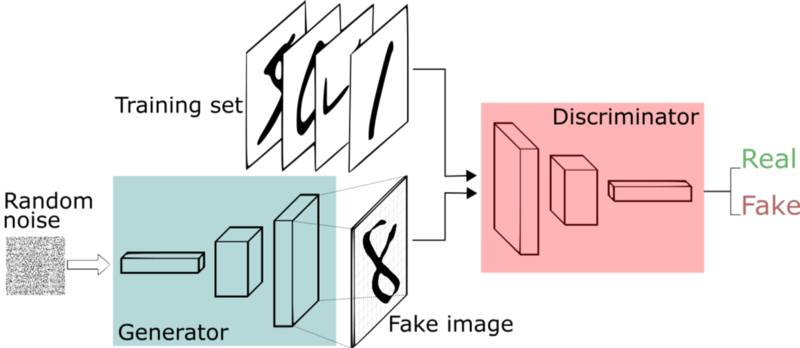
\includegraphics[width=0.7\textwidth]{images/gan.png}
		\caption{}
		\label{fig:gan_arch}
	\end{subfigure}
	\begin{subfigure}[b]{1.\textwidth}
		\centering
		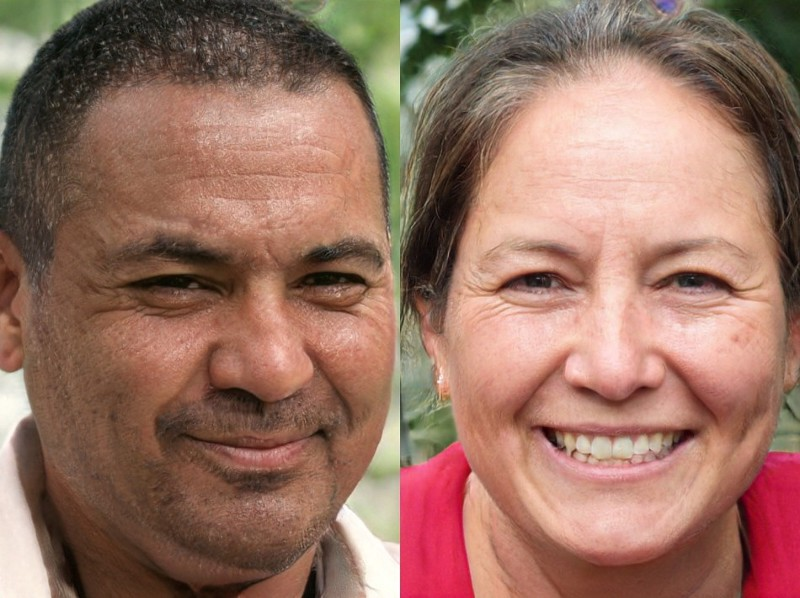
\includegraphics[width=0.5\textwidth]{images/Nvidia/SelectedGenerated.png}
		\caption{}
		\label{fig:gan_sample}
	\end{subfigure}
	\caption{
		روند کلی \gan{}
		(\subref{fig:gan_arch})
		و نمونه تصاویر تولید شده توسط این روش (\subref{fig:gan_sample})
		\cite{gan_nvidia}
	}
\end{figure}
شمایی از نحوه عملکرد این روش در شکل \ref{fig:gan_arch} آمده است؛ همچنین تصاویر شکل \ref{fig:gan_sample} توسط چنین شبکه‌ای تولید شده است که تصاویر بسیار طبیعی هستند.
\\
همان طور که در شکل \ref{fig:gan_arch} مشخص است، شبکه مولد،
\trans{نوفه}{Noise}
را به تصویر تولید می‌کند. در واقع عامل تصادفی در تصادفی بودن \noise{} اولیه نهفته است. اما در حوزه متن معمولا مدل‌های مولد \noise{}‌ای را دریافت نمی‌کنند چرا که عامل اصلی در نمونه‌گیری هر کلمه در هر زمان وجود داشته و چندان نیازی به \noise{} ورودی نیست.
\section{چالش‌ها} \label{chap1:challenge}
\subsection{ 
    رفتار \meanseeking{} روش \maxlikelihood{}}
همان طور که در بخش \ref{chap1:sec:approaches} اشاره شد، از آنجا که در روش \maxlikelihood{} در واقع فاصله $KL(\prob_\text{Data} ~ || Q)$ را کمینه می‌کنیم (زمانی که به دنبال یادگیری $Q$ هستیم)، لازم است تا رفتار مدل در حالتی که ظرفیتی کمتر از پیچیدگی داده دارد را بررسی کنیم. رفتار این فاصله، به گونه‌ای است که Q را به سمتی سوق می‌دهد تا به تمام نقاطی که در $\prob_\text{Data}$ احتمالی دارند، احتمالی نسبت دهد؛ اما نکته نامطلوب آن است که در صورت کمتر بودن ظرفیت مدل نسبت به پیچیدگی داده، برای احتمال نسبت دادن به تمام نقاط داده آموزشی، به نقاطی که در توزیع اصلی داده، احتمالی ندارند نیز احتمال نسبت می‌دهد.
\begin{figure}[h]
	\centering
	\begin{subfigure}[t!]{.4\textwidth}
		\centering
		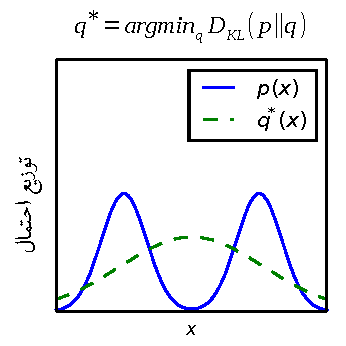
\includegraphics[height=1.\textwidth]{images/KLvsReverseKL_KL.pdf}
		\caption{}
		\label{fig:meanseeking_KL}
	\end{subfigure}
	\begin{subfigure}[t!]{.4\textwidth}
		\centering
		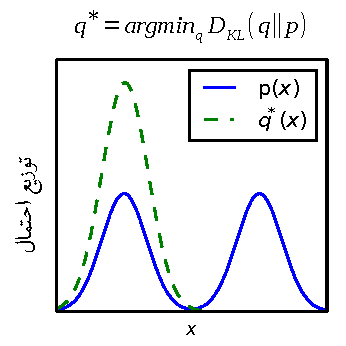
\includegraphics[height=1.\textwidth]{images/KLvsReverseKL_RKL.pdf}
		\caption{}
		\label{fig:meanseeking_RKL}
	\end{subfigure}
	\caption{
		تفاوت رفتار فاصله \lr{KL} (\subref{fig:meanseeking_KL}) و \lr{KL} برعکس (\subref{fig:meanseeking_RKL}) در نحوه یادگیری مدل.
	}
\end{figure}
همان طور که در شکل \ref{fig:meanseeking_KL} دیده می‌شود، ممکن است نقطه‌ای بیشینه احتمال داشته باشد که در توزیع اصلی احتمالی ندارد. به این رفتار روش \maxlikelihood{}، رفتار 
\trans{میانگین جویانه}{Mean Seeking}
 گفته می‌شود. این درحالیست که \lr{KL} برعکس، رفتاری معکوس داشته و در این حالت تنها یکی از قله‌ها را پوشش خواهد داد.
\subsection{ناپایداری و مشکلات \gan{}}
دو مشکل در نحوه آموزش \gan{} نهفته است. اول آنکه با توجه به نحوه آموزش مولد، تنها کافیست مولد نمونه‌ای تولید نماید که \discriminator{} توانایی تشخیص آن از نمونه واقعی را ندهد. در واقع طبیعی بودن نمونه‌ها در روش دیده شده است اما تنوع خیر؛ از سوی دیگر می‌تواند این رفتار به صورت تناوبی بین بعضی نمونه‌ها در حین آموزش جابه‌جا شود. برای مثال اگر هدف یادگیری تصویر قرمز رنگ شکل \ref{fig:gan_train} باشد، ممکن است مسیر آموزش به حالت شکل \ref{fig:gan_bad_train} درآمده و بین بعضی قله‌های داده جابه‌جا شود و از سوی دیگر نیز ممکن است به صورت شکل \ref{fig:gan_good_train} آموزش داده شود که حالتی پایدار است. اگر روند آموزش دچار چنین مشکلی شود، مدل دچار
\trans{چسبیدگی به قله}{Mode Collapse}
شده است \cite{wgan, gan}.
\begin{figure}[h]
	\centering
	\begin{subfigure}[h]{.7\textwidth}
		\centering
		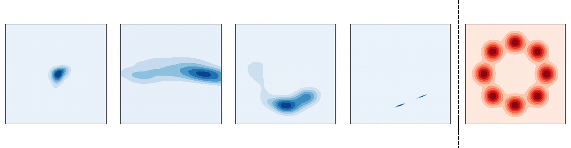
\includegraphics[width=1.\textwidth]{images/GANBadTrain.pdf}
		\caption{}
		\label{fig:gan_bad_train}
	\end{subfigure}
	\begin{subfigure}[h]{.7\textwidth}
		\centering
		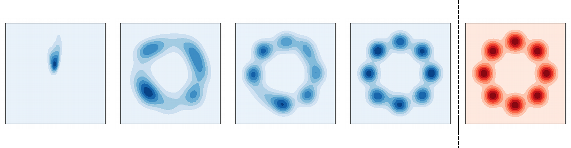
\includegraphics[width=1.\textwidth]{images/GANGoodTrain.pdf}
		\caption{}
		\label{fig:gan_good_train}
	\end{subfigure}
	\caption{
		نمونه‌ای آموزش ناپایدار (\subref{fig:gan_bad_train}) و پایدار
		(\subref{fig:gan_good_train}) \gan{} \cite{numerics_gan}.
	}
	\label{fig:gan_train}
\end{figure}
\\
مشکل دوم نیز کنترل میزان آموزش \discriminator{} و \generator{} در مقابل یکدیگر است. در صورتی که \discriminator{} بیش از حد آموزش داده شود به طوری که به راحتی نمونه‌های واقعی را از مصنوعی تشخیص دهد، گرادیانی از \discriminator{} به مولد منتقل نشده و آموزش شبکه متوقف خواهد شد. به منظور رفع این مشکل‌ها، راه حل‌های متفاوتی همچون \wgan{}
\LTRfootnote{\lr{Wasserstein Generative Adversarial Network (WGAN)}}
  ارائه شده است \cite{wgan}.
\subsection{عدم توجه به فضای نهان} \label{chap1:latent_ignore}
زمانی که از مدل‌های با فضای نهان استفاده می‌شود، به دنبال یافتن فضای نهانی تفسیرپذیر و تاثیرگذار بر روی خروجی \decoder{} هستیم؛ اما در صورت بالا بودن ظرفیت \decoder{} ممکن است مستقل از فضای نهان، توزیع داده اصلی را فرا بگیرد. در این صورت فضای نهان نه تفسیرپذیر و نه تاثیرگذار بر روی خروجی \decoder{} بوده و عملا با یک مدل زبانی بدون فضای نهان برابری خواهد کرد. این مشکل نیز مورد توجه محققان بوده و روش‌های متفاوتی از جمله \wae{}
 \LTRfootnote{\lr{Wasserstein Autoencoder (WAE)}}
  ارائه شده است \cite{wae, infovae, vae_lagging, vae_lossy}.
\subsection{گذر گرادیان در نمونه‌برداری و \argmaxphrase{}}
از آنجا که در حوزه مدل زبانی با نمونه‌گیری از توزیع کلمات سر و کار داریم، در روش‌هایی مانند \gan{} با مشکل مواجه خواهیم بود. در واقع به دلیل اینکه نمونه‌گیری عملیاتی مشتق نا‌پذیر است، امکان گذر گرادیان از این عملیات به عقب وجود ندارد. برای مثال در روش \gan{}، تابع هدف مدل مولد، تولید نمونه‌هاییست که از نظر \discriminator{} واقعی به نظر رسند. بنابراین بایستی از مولد نمونه‌برداری کرده و سپس احتمال واقعی بودن نمونه‌ها توسط \discriminator{} ارزیابی شود. حال برای آموزش دادن پارامتر‌های مولد نیاز است تا گرادیان از \discriminator{} به مولد منتقل گردد؛ اما در این مسیر عملیات نمونه‌برداری وجود دارد. مشکل مشابهی نیز هنگام 
\trans{آرگومان بیشینه یابی}{Argmax}
 رخ می‌دهد. برای رفع این مشکل نیز راه‌حل‌هایی همچون بهره‌گیری از یادگیری تقویتی و یا روش‌هایی تقریبی همچون \lr{Gumbel Softmax} و \lr{Soft-argmax} ارائه شده‌اند اما روش یادگیری تقویتی واریانس گرادیان را افزایش داده و روش‌های تقریبی نیز دارای پارامتر‌هایی هستند که تنظیم آن‌ها نیازمند توجه و دقت است \cite{seqgan, gumbel}
\subsection{عدم تطابق شرط با جمله تولیدی}
مشکل دیگری که ممکن است در روش‌های مبتنی بر \likelihood{} پیش آید، احتمال ناهمخوانی شرط با جمله تولیدی است. از آنجا که معمولا تطابق جمله خروجی با شرط چک نمی‌شود، ممکن است این اتفاق نامطلوب رخ دهد. لازم به ذکر است که در روش \gan{} انتظار چنین رخدادی وجود ندارد چرا که این موضوع توسط \discriminator{} تصحیح می‌شود \cite{toward}.
\section{هدف پژوهش}
با توجه به تعریف مسئله در بخش \ref{chap1:prob_define} و چالش‌های معرفی شده در بخش \ref{chap1:challenge} به دنبال ارائه روشی برای آموزش شبکه‌های مولد شرطی بوده که کمتر با چالش‌های ارائه شده مواجه شود و جملات تولیدی چه به لحاظ کیفیت و چه به لحاظ تطابق با شرط از سطح قابل قبولی برخوردار باشند.
\\
به این منظور در یک رویکرد، سعی در آموزش مدل مولد با فضای نهان شرطی به طوری که فضای نهان به ازای مقادیر مختلف شرط تقسیم گردد، خواهیم داشت؛ اما در رویکرد دوم، فضای نهان از شرط 
\trans{مستقل}{Disentangle}
بوده و نسبت به مقادیر مختلف شرط تقسیم نخواهد شد. علاوه بر این از معماری‌های نوینی همچون \transformer{}، روش‌هایی همچون \wae{} برای جلوگیری از مشکل عدم توجه به فضای نهان و همچنین رویکرد‌های آموزش مدل‌های مولدی که کمتر مورد توجه بوده‌اند اما ویژگی‌های متناسب با فضای مسئله را دارند، استفاده خواهد شد.

\section{ساختار پایان‌نامه}
در فصل \ref{chap2}، پس از معرفی تعدادی فاصله بین توزیع‌های به عنوان پیشنیاز، به دلیل شباهت مدل‌های زبانی شرطی به غیر شرطی، ابتدا مدل‌های غیر شرطی تحت عنوان مدل‌های با فضای نهان و بدون فضای نهان تشریح شده و در انتها نیز معماری نوینی تحت عنوان \transformer{} معرفی می‌گردد. از آنجا که در روش پیشنهادی از نوعی مدل‌های مولد که پیش‌تر مورد توجه نبوده‌اند استفاده گردیده است، به معرفی این دسته از مدل‌های مولد نیز پرداخته خواهد شد. در فصل \ref{chap3} نیز پس از بررسی اجمالی مدل‌های معرفی شده، مدل پیشنهادی ارائه شده و در فصل  \ref{chap4} پس از معرفی داده و معیارهای ارزیابی مورد بررسی قرار گرفته و نتایج گزارش شده است. در نهایت نیز ضمن ارائه جمع‌بندی از کارهای انجام شده، پیشنهاداتی جهت ادامه تحقیقات معرفی خواهد شد.





\chapter{پژوهش‌های پیشین}\label{chap2}
\minitoc

در این فصل برخی مدل‌های ارائه شده مرتبط با مسئله گپ‌زن دانش  ارائه و بررسی خواهند شد. در انتها نیز برخی دادگان جمع‌آوری شده در طی سالیان اخیر که می‌توانند برای مساله گپ‌زن دانش مفید واقع شوند معرفی شده اند.

\section{مدل‌های گپ‌زن دانش بنیان}\label{intro}

\subsection{مدل پیشنهاد شده توسط وینیالز}

این مدل در سال ۲۰۱۵ و بر پایه معماری دنباله به دنباله با استفاده از شبکه LSTM 
دو لایه با اندازه 
\trans{Hidden State }{حالت نهان}
۴۰۹۶
ارائه شد
\cite{A_Neural_Conversational_Model}.
این مدل در واقع فاقد منبع دانش خارجی است و صرفا از شبکه آموزش دیده شده روی دادگان آموزشی تشکیل شده است. اما اهمیت ذکر این مدل در اینجا، به دلیل نشان دادن این حقیقت است که حتی مدل‌های فاقد منبع دانش نیز  علاوه بر تقلید 
\trans{دستور زبان}{grammar}
 مکالمه انسانی، قادرند تا مقداری از حقایق جهان را در شبکه خود ذخیره کنند.
 برای مثال،‌ نمونه‌ای از گفتگوی چالشی دانش‌محور عامل انسانی با این مدل در شکل
 \ref{fig:chap2:Vinyals1}
 آورده شده است.

\begin{figure}[h]
	\centering
	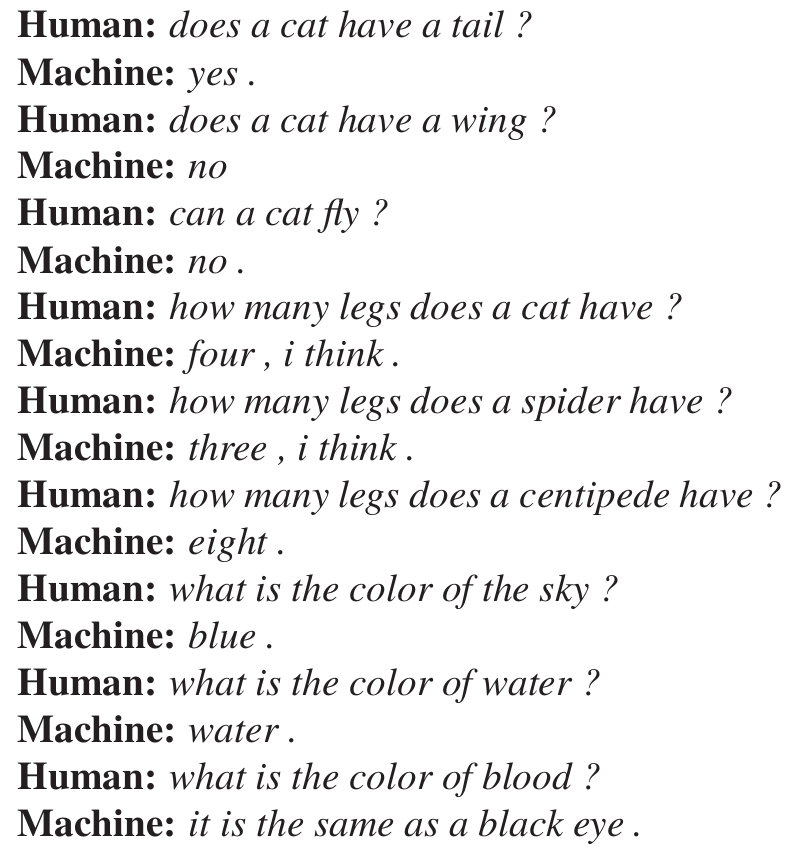
\includegraphics[width=0.75\textwidth]{images/chap2/Vinyals1.png}
	\caption{
		نمونه‌‌ای از گفتگوی چالشی دانش‌محور عامل انسانی با مدل وینیالز
		\cite{A_Neural_Conversational_Model} 
	}
	\label{fig:chap2:Vinyals1}
\end{figure}

همانطور که در شکل
\ref{fig:chap2:Vinyals1}
مشاهده‌ می‌شود مدل در پاسخ به سوالاتی مانند تعدادی پا‌های گربه و یا رنگ آسمان توانسته‌ است به خوبی پاسخ درست را خروجی دهد، حال آن که در موارد دیگری نظیری رنگ آب و یا تعداد پاهای عنکبوت نتوانسته‌است به موفقیت دست پیدا کند.

مدل وینیالز را می‌توان یکی از اولین تلاش‌های موثر در دستیابی به گپ‌زن دامنه باز دانست. این مدل سعی کرد تا با آموزش بر روی دادگان عظیم 
\lr{OpenSubtitle}
به این مهم دست یابد و توانایی این مدل در برخی استنتاج‌‌ها و پاسخگویی به سوالات چالشی دانش‌محور را نیز می‌توان به نوعی از تاثیرات حجم عظیم دادگان‌ آموزشی آن دانست. پژوهش وینیالز علاوه بر موارد فنی مطرح شده، در زمینه آزمایش و ارزیابی مدل خود از آزمایشات جالب توجه و چالش بر‌انگیز  انجام مکالمات چالش برانگیز 
(نظیر آن‌چه که در شکل 
\ref{fig:chap2:Vinyals1}
به نمایش درآمد
)
استفاده کرد که می‌تواند نمونه‌ای‌ مناسب برای ارزیابی مدل‌های بعد از خود باشد. 

\subsection{مدل پیشنهاد شده توسط قزوینی نژاد}


\subsection{پیش‌نیازها}
\iffalse
	قرارداد می‌کنیم توزیع $P$ مربوط به توزیع داده واقعی باشد و در مقابل آن به دنبال یافتن توزیع $Q$ هستیم که تا حد ممکن نزدیک به $P$ باشد.
	از آنجا که در طول متن گزارش، فاصله‌های گوناگونی مورد استفاده قرار گرفته است، در ابتدا آن‌ها تعریف می‌کنیم. در تمامی تعاریف، P مربوط به توزیع اصلی و Q مربوط به توزیعی است که یاد گرفته می‌شود.
\fi
\subsubsection{معیارهای فاصله بین دو توزیع} \label{chap2:divs}
پیش از توضیح روش‌های مختلف ابتدا  لازم به ذکر است تمامی این فواصل بین دو توزیع $p$ و $q$ تعریف شده‌اند.
\\
\bff{فاصله \lr{KL}} \cite{bishop}:
\begin{gather} \label{eq: kl}
	KL (p ~ || ~ q)   = \sum_x p(x) \log \frac{p(x)}{q(x)}
\end{gather}
اگر $p$ توزیع داده باشد و به دنبال یادگیری $q$ باشیم، کمینه کردن فاصله فوق همان روش \maxlikelihood{} خواهد بود.
\\
\bff{فاصله \lr{KL} برعکس}:
\begin{gather} \label{eq: rkl}
	KL (q ~ || ~ p)   = \sum_x q(x) \log \frac{q(x)}{p(x)}
\end{gather}
مجددا اگر $p$ توزیع داده باشد، از آنجا که دسترسی به آن وجود ندارد، فاصله فوق به صورت مستقیم قابل بهینه‌سازی نیست.
\\
\bff{فاصله \lr{Jensen Shannon}}:
\begin{gather} \label{eq: js}
	JS (p ~ || ~ q)   = KL(p ~ || ~ \frac{p + q}{2}) + KL(q ~ || ~ \frac{p + q}{2})
\end{gather}
این فاصله بر خلاف دو فاصله قبلی، نسبت به جابه‌جایی $p$ و $q$ حساس نبوده و \gan{} در تئوری، این فاصله را کمینه می‌کنند \cite{gan}.
\\
\bff{فاصله
	\trans{واسرشتاین}{Wasserstein}}:
فرض کنید می‌خواهید تعداد مشخصی جعبه که به ترتیب خاصی بر روی یکدیگر و کنار هم قرار گرفته‌اند را به مکانی دیگر منتقل کنید. برای مثال طبق شکل \ref{fig:chap2:wasser1} میخواهید مربع‌های سمت چپ را به مکان‌های با نقطه‌چین مشخص شده منتقل کنید. به صورت‌های مختلفی می‌توان این کار را انجام داد. دو نمونه از این جابه‌جایی در شکل \ref{fig:chap2:wasser2} آمده است.
\begin{figure}[h]
	\centering
	\begin{subfigure}[t]{.7\textwidth}
		\centering
		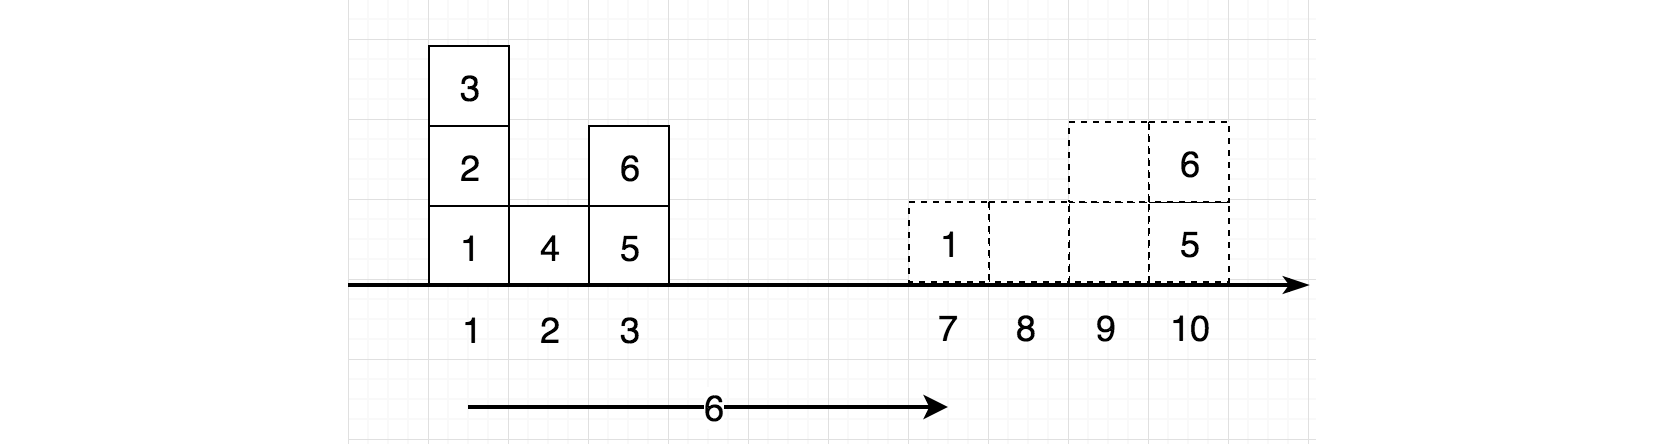
\includegraphics[width=1.\textwidth]{images/wasser2.png}
		\caption{}
		\label{fig:chap2:wasser1}
	\end{subfigure}

	\begin{subfigure}[t]{.6\textwidth}
		\centering
		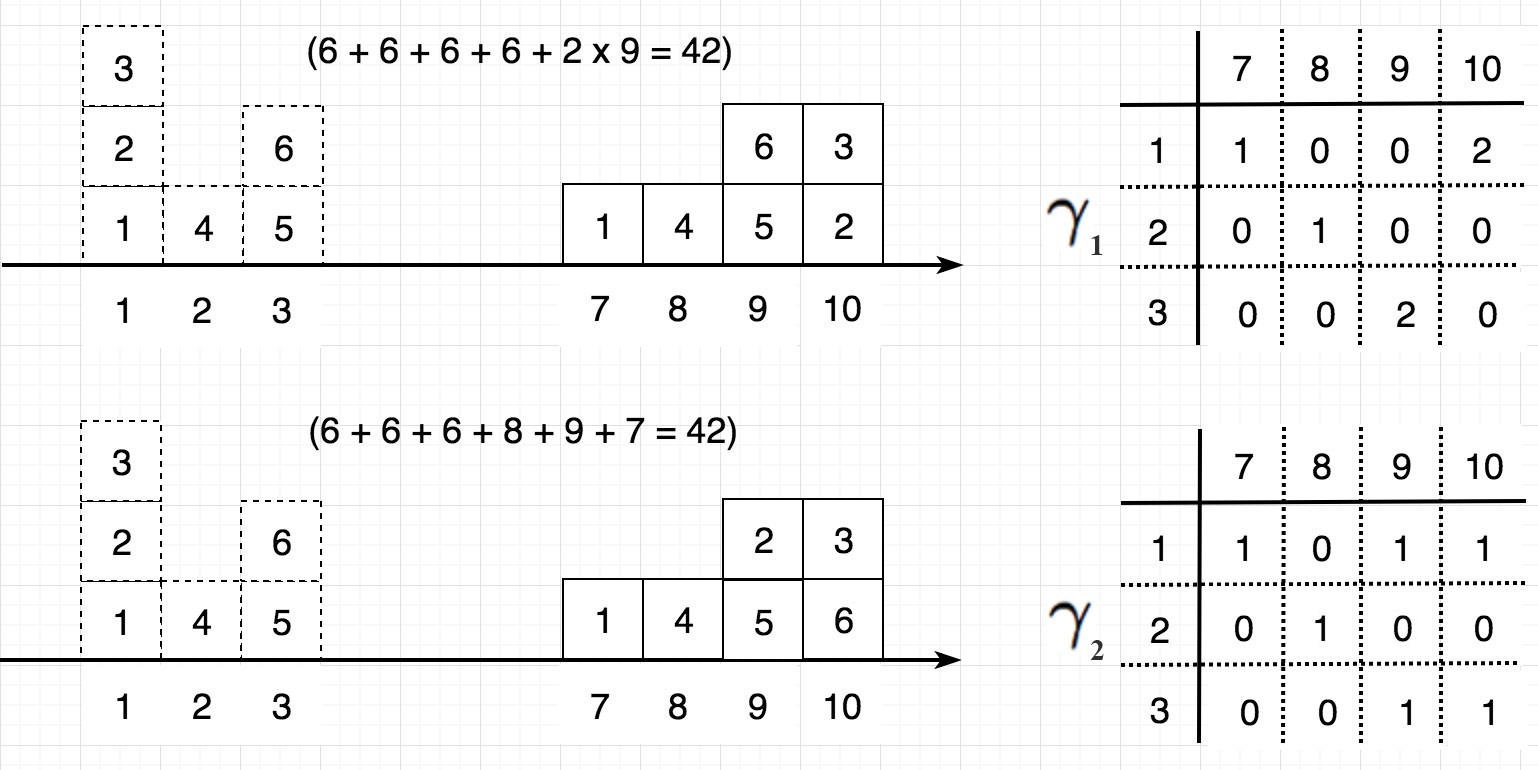
\includegraphics[width=1.\textwidth]{images/wasser1.jpeg}
		\caption{}
		\label{fig:chap2:wasser2}
	\end{subfigure}
\caption{
    مثالی از دو توزیع \subref{fig:chap2:wasser1} و 
    \transportplan{} 
    بین دو توزیع \subref{fig:chap2:wasser2}}
\end{figure}
اگر $\gamma$ را یک
\trans{طرح جابه‌جایی}{Transport Plan}
بنامیم که به صورت جدولی که سطرها مکان اولیه جعبه‌ها و ستون‌ها مکان ثانویه جعبه‌ها نشان داده و هر خانه آن نشان دهنده تعداد جعبه‌ی جابه‌جا شده از نقطه اولیه به ثانویه است، جمع عناصر این جدول برابر هزینه جابه‌جایی کلیه جعبه‌ها خواهد بود. از آنجا که \transportplan{} واحدی به این منظور وجود ندارد، \transportplan{} با کمترین هزینه جابه‌جایی برابر فاصله \wasser{} بین حالت اولیه و ثانویه جعبه‌ها است.
\\
به منظور تعریف دقیق‌تر، اگر دو توزیع به نام‌های $q$ و $p$ داشته باشیم، فاصله \wasser{} برابر کمترین هزینه جابه‌جایی برای جابه‌جایی جرم توزیع $p$ به $q$ خواهد بود.
اگر مجموعه تمام توزیع‌های توام $\gamma(x,y)$ که توزیع‌های \marginal{} آن به ترتیب برابر $p$ و $q$ باشد را با $\Pi(p,q)$ نشان دهیم، فاصله \wasser{} به صورت زیر تعریف می‌شود:
\begin{align}
	W_c(p,q) = \inf_{\gamma(x,y) \in \Pi(p,q)} \expected_{(x,y) \sim \gamma(x,y)} [ c(x,y) ]
\end{align}
و $c$ یک متر تعریف شده بر روی این فضا و اندازه‌گیرنده هزینه جابه‌جایی بین دو نقطه است. به طور شهودی توزیع توام $\gamma$ نشان دهنده جرم جابه‌جا شده از نقطه $x$ به نقطه $y$ است به طوری که تمام جرم از توزیع $p$ به توزیع $q$ منتقل شود. در حالتی که $c = ||x-y||$ باشد، به فاصله فوق فاصله \earthmover{} نیز گفته می‌شود.
\\
از آنجا که کمینه کردن فاصله فوق معمولا سخت است، طبق فرم دوگان \lr{Kantorovich-Rubinstein } فاصله \earthmover{} برابر است با \cite{wgan}:
\begin{align}
	W(p, q) = \sup_{||f||_L \leq 1} \expected_{x \sim p(x)}[f(x)] - \expected_{x \sim q(x)}[f(x)]
\end{align}
که سوپریمم بر روی تمام توابع $f$ با ضریب \lipschitz{} حداکثر یک گرفته شده است. شرط \lipschitz[K-]{} که به صورت
$|f(x) - f(y)| \leq K |x - y|$
به ازای تمام $x$ و $y$ ها تعریف می‌شود به طور شهودی به معنای توابعی است که چندان تغییرات شدیدی ندارند.
\\
از این فاصله به عنوان تابع هدف جدید در \gan{} استفاده شده که به \wgan{} معروف است. نکته قابل توجه این است که چون تابع $f$ فوق چندان انحنای شدیدی ندارد، حتی در صورت دور بودن توزیع داده واقعی و مصنوعی، همچنان تابع $f$ به صورت محلی احتمالا خطی بوده و گرادیان از \discriminator{} به \generator{} بر خواهد گشت \cite{wgan}. نمایی از این تفاوت گرادیان دو نوع  \gan{} در شکل \ref{fig:chap2:wgan1} مشخص است.
\begin{figure}[h]
	\centering
	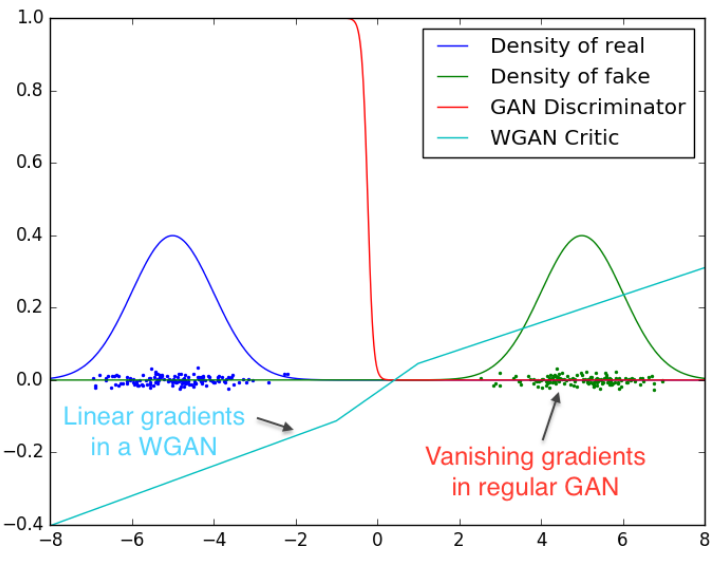
\includegraphics[width=0.5\textwidth]{images/wgan1.png}
	\caption{
        تفاوت خروجی \discriminator{} در \gan{} عادی و \wgan{} (\lr{WGAN})
        \cite{wgan}
    }
	\label{fig:chap2:wgan1}
\end{figure}
\\
\bff{فاصله 
    \trans{بیشینه اختلاف میانگین}{Maximum Mean Disrepancy (\mmd{})} (\mmd{})}:
برای تابع کرنل مثبت معین 
\trans{‎با قابلیت بازتولید}{Reproducing}
$k: ‎\mathcal{Z} ‎‎\times \mathcal{Z} ‎\rightarrow ‎\mathbb{R}‎‎$
رابطه ‎\mmd{} به شکل زیر تعریف می‌شود:
\begin{gather}
	\mathsf{MMD}_k(p, q) = {\vert \vert \int_\mathcal{X} k(x, .) dp(x) - \int_\mathcal{X} k(x, .) dq(x) \vert \vert}_{\mathcal{H}_k}
\end{gather}
به طوری که $‎\mathcal{H}‎_k$، یک 
\trans{کرنل با قابلیت بازتولید در فضای هیلبرت}{Reproducing ‎ Kernel ‎ Hilbert ‎ Space (RKHS)}،
برای توابع از $‎\mathcal{X}‎$ به اعداد حقیقی است. اگر تابع $k$ ویژگی‌های مشخصی را داشته باشد، ‎\mmd{}‎ را به یک متر تبدیل کرده و این امکان را فراهم می‌کند تا از این متر به عنوان تابع هزینه برای کمینه کردن فاصله دو توزیع $p$  و $q$  بهره برده شود. از آنجا که رابطه بالا به طور مستقیم قابل محاسبه و بهینه‌سازی نیست، از تخمین‌گر 
\trans{نااریب}{Unbiased}
 زیر استفاده می‌گردد. اگر $n$ نمونه از دو توزیع $p$ و $q$ داشته و به ترتیب با $x_i$ و $‎\tilde{x}_i$ نشان داده شوند،‌خواهیم داشت:
\begin{align}
	\mathsf{MMD}_k(x_{1,2,...,n};\tilde{x}_{1,2,...,n}) = & \frac{1}{n(n-1)} \sum_{l \neq j} k(x_l, x_j) +
	\frac{1}{n(n-1)} \sum_{l \neq j} k(\tilde{x}_l, \tilde{x}_j)                            \nonumber         \\
	                                                      & - \frac{1}{n ^ 2} \sum_{l, j} k(x_l, \tilde{x}_j)
\end{align}
فاصله فوق با کرنل
$k(x, y) = \frac{C}{C + ||x - y||^2_2}$
برای فاصله بین دو توزیع گاوسی کاربرد دارد و به خوبی عمل می‌کند \cite{wae}.

\section{مدل‌های زبانی بدون فضای نهان}
\subsection{مدل زبانی پایه (\teacherforcing{})}
مدل \teacherforcing{} شاید ساده‌ترین دسته از مدل‌های تولید متن با استفاده از شبکه‌های عصبی باشد. آموزش این مدل‌ها مبتنی بر بیشینه کردن \likelihood{} داده آموزش در مدل است \cite{teacher_force} اگر پارامترهای مدل را با $‎\theta$ نشان دهیم، تابع هزینه این مدل به صورت زیر است:
\begin{equation}\begin{split}
		L_{MLE} = -\expected_{\bff{x} \sim p_{data}(\bff{X})} [\log p_\theta (\bff{x})] = -\expected_{\bff{x} \sim p_{data}(\bff{X})} [\log p_\theta (\bff{x}_1) + \sum_{t=2}^{T}  \log p_\theta (\bff{x}_t|\bff{x}_1, ..., \bff{x}_{t-1})].
	\end{split}\end{equation}

\begin{figure}[H]
	\centering
	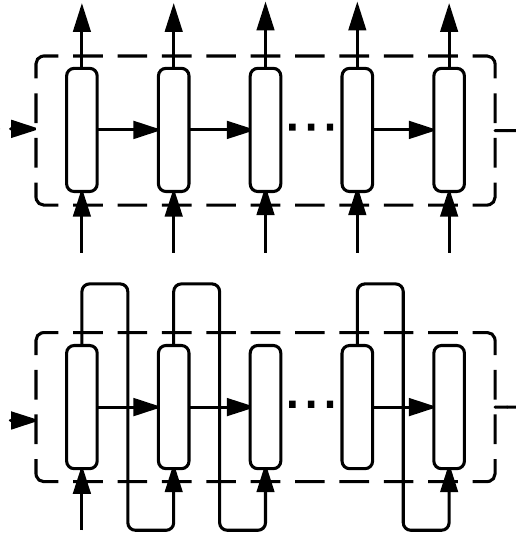
\includegraphics[width=0.25\textwidth]{images/teach-prof.png}
	\caption{
		تفاوت بین آموزش و آزمون مد‌ل جبر معلم. شکل بالا مربوط به زمان آموزش و شکل پایین مربوط به زمان آزمون است. \cite{prof_force}.}
	\label{fig:chap2:expbias}
\end{figure}

به عبارت دیگر، در هر زمان درست‌نمایی هر کلمه را با داشتن کلمات قبلی بیشینه می‌کنیم. \\
همان‌طور که از روابط تابع هزینه مشخص است، آموزش این دسته از مدل‌ها ساده بوده اما دچار پدیده‌ای به نام 
\trans{اریبی مواجهه}{Exposure bias}
 هستند \cite{ prof_force, s_sampling}. این مشکل ناشی از تفاوت رفتار با مدل حین آموزش و حین آزمون است. همان طور که در شکل \ref{fig:chap2:expbias} مشخص است، حین آموزش، در هر زمان، کلمات کاملا درست تحویل مدل شده، در حالی که در زمان آزمون ورودی شبکه در هر زمان، با استفاده از نمونه‌گیری از خود مدل در زمان قبل ساخته می‌شود. از آنجا که مدل مفهوم کاملا درستی را نیاموخته است، کلمه‌ی تولید شده برای ورود به زمان بعد، کلمه کاملا صحیحی نبوده و چنین رفتاری باعث می‌شود تا مدل، ورودی‌ای را دریافت کند که دارای مقداری خطا بوده که در زمان آموزش مانند آن را ندیده است (در زمان آموزش کلمات کاملا صحیح ورودی شبکه بوده‌اند)؛ این رفتار در طول تولید هر کلمه از یک جمله با هم تجمیع شده و در نهایت منجر به تولید جمله‌ای نه چندان صحیح خواهد شد.\\
به منظور رفع این مشکل، روش‌های متفاوتی ارائه شد \cite{prof_force, s_sampling, seqgan} که در بخش \ref{chap2:seqgan} به عنوان یکی از راه‌حل‌ها به آن پرداخته خواهد شد.
از دیگر مشکلات این روش باید به تفاوت تابع هزینه و معیار ارزیابی اشاره کرد؛ به عبارت دیگر اگر معیار ارزیابی، معیاری مانند \lr{BLEU} باشد، هدف ارزیابی کسب امتیاز بالاتر \lr{BLEU} است و نه افزایش درست‌نمایی داده آموزش و لزوما افزایش درست‌نمایی به افزایش ‌\lr{BLEU} منجر نمی‌شود.
\subsection{مدل زبانی با استفاده از \gan{}}
شاید \gan{} یکی از مطرح‌ترین و موفق‌ترین مدل‌های مولد حال حاضر باشند. این شبکه‌ها که مجددا ابتدا در حوزه تصویر معرفی شدند، از دو بخش کلی تشکیل شده اند \cite{gan}؛ بخش 
\generator{}
  و بخش 
\discriminator{}.
  همان‌طور که از نام‌گذاری آن‌ها مشخص است، مولد وظیفه تولید نمونه‌های مصنوعی و \discriminator{} وظیفه تشخیص نمونه مصنوعی از واقعی را دارد. نحوه آموزش آن‌ها به این صورت است که مولد سعی در تولید نمونه‌های شبیه به داده واقعی داشته و \discriminator{} در جهت مخالف سعی در شناسایی این نمونه‌ها دارد. در واقع نوعی 
\trans{بازی کمینه-بیشینه}{Min-max game}
بین مولد و \discriminator{} در جریان است. تابع هدف این مدل به شرح زیر است \cite{gan}:
\begin{equation} \label{eq:gan}
	\begin{split}
		V_{GAN} (G, D) = \expected_{\bff{x} \sim p_{data}(\bff{X})} [\log D(\bff{x})] + \expected_{\bff{z} \sim p(\bff{Z})} [\log (1 - D(G(\bff{z})))]
	\end{split}
\end{equation}
که  $p(\bff{z})$ توزیع پیشین تعریف شده بر روی نویز $\bff{z}$،
$G(\bff{z})$
تابع مولد (تبدیل کننده نویز $\bff{z}$ به نمونه $\bff{x}$)، $D(\bff{x})$ تابع \discriminator{} بوده و این رابطه برحسب $G$ کمینه و $D$ بیشینه می‌گردد.\\
اگر $q_G(\bff{x})$ نشان دهنده توزیع حاصل از اعمال تابع $G(\bff{z})$ به توزیع پیشین $p(\bff{z})$ باشد؛ نشان داده شده است که نقطه بیشینه کننده رابطه \ref{eq:gan} بر حسب $D$، به صورت زیر است \cite{gan}:
\begin{gather}
	D_G^*(\bff{x}) = \frac{p_{data}(\bff{x})}{p_{data}(\bff{x}) + q_G(\bff{x})}
\end{gather}
با فرض رسیدن به \discriminator{} بهینه، کمینه کردن $V(D^*_G,G)$ معادل کمینه کردن فاصله \lr{Jensen Shannon} بین $p_{data}(\bff{x})$ و $q_G(\bff{x})$ خواهد بود.

همان طور که اشاره شد \gan{}، ابتدا در حوزه تصویر معرفی شده و به دلیل عدم امکان عبور گرادیان که در ادامه شرح داده خواهد شد، چندان در حوزه متن موفق نبود. این مشکل از نحوه آموزش نشأت می‌گیرد. همان طور که در روابط تابع هزینه مشخص است، \discriminator{} باید به نمونه‌های تولید شده توسط مولد عددی نزدیک به صفر نسبت دهد. آنچه که باید در آموزش و الگوریتم 
\trans{گرادیان کاهشی تصادفی}{Stochastic gradient descent}
محاسبه شود، محاسبه مشتق تابع هزینه نسبت به پارامتر‌های شبکه مولد است؛ اما از آنجا که شبکه مولد مستقیما در تابع هزینه شرکت نکرده و نمونه‌های تولیدی آن شرکت می‌کنند و عملیات نمونه‌گیری در فضای گسسته عملیاتی مشتق‌ناپذیر است، بنابراین امکان گذر گرادیان از تابع هزینه (شبکه \discriminator{}) به شبکه مولد به سادگی وجود ندارد. در واقع شبیه چنین مشکلی در شبکه‌های \vae{} نیز وجود دارد اما با تکنیکی به نام
\trans{پارامتری‌سازی مجدد}{Reparameterization}
که منبع تزریق عامل تصادفی (نمونه‌گیری) را از مسیر انتقال گرادیان خارج می‌کند، حل شده است \cite{vae}.\\
به منظور حل این مشکل نیز رویکرد‌های متفاوتی ارائه شده است که به یکی و شاید معروف‌ترین از آن‌ها اشاره خواهد شد \cite{seqgan, gumbel}.\\
\subsubsection{\lr{SeqGAN}}  \label{chap2:seqgan}
در روش \lr{SeqGAN} راه حل ارائه شده برای مشکل گذر گرادیان الهام گرفته شده از حوزه 
\trans{یادگیری تقویتی}{Reinforcement Learning}
است \cite{seqgan}؛ در واقع همین مشکل به نوعی دیگر در حوزه یادگیری تقویتی مطرح است و با روشی به نام روش 
\trans{گرادیان سیاست}{Policy gradient}
 رفع شده است. ساختار یک مسئله حوزه یادگیری تقویتی شامل ۴ بخش است که با تعریف تمام بخش‌های آن، ‌می‌توان بخش آموزش مولد در \gan{} را به عنوان آموزش یک عامل با روش \reinforce{} دید. این بخش‌ها شامل موارد روبرو هستند: فضای حالت عامل ($S$)، فضای عمل عامل ($A$)، 
\trans{تابع گذار}{Transition function}
(\lr{$T(s,a)$})
و 
\trans{تابع پاداش}{Reward function}
(\lr{$R(s,a)$}).
\begin{equation}\begin{split}
		\nonumber
		T: S \times A \rightarrow S\\
		R: S \times A \rightarrow \mathbb{R}
	\end{split}\end{equation}
در اینجا حالت فعلی عامل، 
\trans{بازنمایی}{Representation}
کلمات تولید شده تا به حال است؛ عمل عامل،‌ کلمه انتخابی بعدی؛ حالت بعدی، تجمیع کلمات قبلی تولید شده و کلمه فعلی و در نهایت تابع پاداش، امتیاز میزان واقعی بودن جمله است که تمایز دهنده به جمله تولیدی نسبت می‌دهد. بدیهی است که تابع گذار تابعی 
\trans{قطعی}{Deterministic}
بوده و پاداش مورد نظر بعد از تولید کامل جمله به عامل داده می‌شود. در این حالت رابطه گرادیان تابع مولد به شکل زیر بدست خواهد آمد \cite{seqgan}.
\begin{equation} \label{eq:seqgan-grad}
	\begin{split}
		\nabla_G L_{GAN} (G, D) &= \nabla_G \expected_{\bff{x} \sim G(\bff{X})} [\log D(\bff{x})]= \expected_{\bff{x} \sim G(\bff{X})} [\log D(\bff{x}) \nabla_G \log G(\bff{x})].
	\end{split}
\end{equation}

\begin{figure}[t]
	\centering
	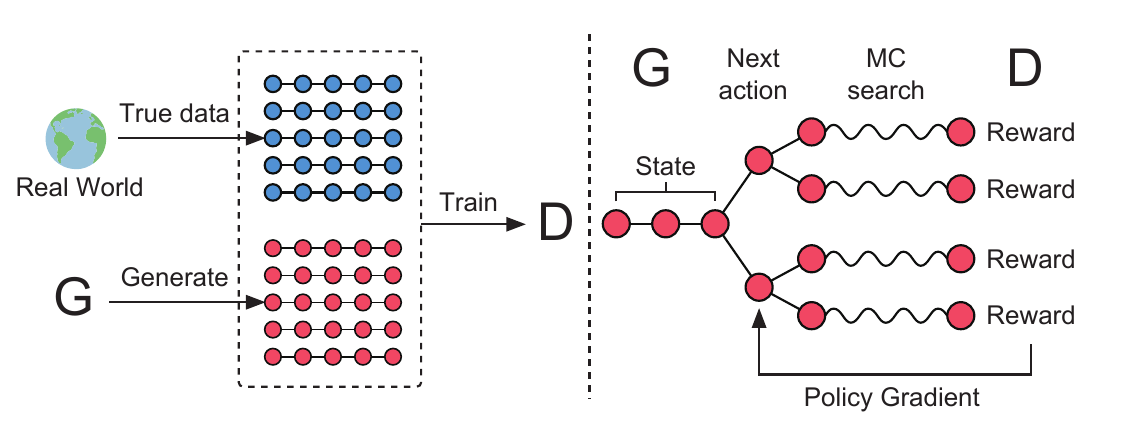
\includegraphics[width=0.5\textwidth]{images/seq-gan.png}
	\caption{
		نمایی نحوه آموزش مدل \lr{SeqGAN}
		\cite{seqgan}.}
	\label{fig:seq-gan}
\end{figure}

همان‌طور که در شکل \ref{fig:seq-gan} و رابطه \ref{eq:seqgan-grad} مشخص است، عامل طبق سیاستی که تا به حال بدست آورده است، تعدادی نمونه ایجاد نموده و به نسبت پاداش دریافتی به ازای هر نمونه، درست‌نمایی نمونه‌های مرتبط را افزایش خواهد داد.\\
نکته قابل توجهی که لازم است به آن اشاره شود، توانایی این روش در حل مشکل \expbias{} است. در واقع از یک سو در هر زمان کلمه بعدی توسط خود مدل تولید می‌شود و از سوی دیگر پاداشی که از \discriminator{} دریافت می‌کند، میزان  واقعی بودن کل جمله است؛ بنابراین اگر جمله تولید شده از نظر \discriminator{}، کیفیت لازم را نداشته باشد، \discriminator{} امتیاز کمتری به آن نسبت خواهد داد و گرادیان متناسب به مولد اعمال خواهد شد. با وجود آنکه این روش مشکل ذکر شده را حل می‌کند، اما فضایی که عامل باید در آن به دنبال یافتن پاداش بیشینه باشد نمایی بوده و همین امر آموزش این دسته از مدل‌ها را با چالش روبرو می‌کند. پیشنهاد ساده‌ای که برای این موضوع ارائه می‌شود استفاده از پیش آموزش به روش \teacherforcing{} است. در واقع ابتدا مدل به یک 
\trans{بهینه محلی}{Local optimum}
رسیده و در فضای نزدیک به آن احتمالا پاداش بیشتری نسبت به حالتی که مدل تصادفی باشد دریافت کرده و به اصلاح خود می‌پردازد.\\
این روش تنها مدل موجود با چنین رویکردی نبوده و روش‌هایی همچون \cite{pg_bleu} از دانش خبره مانند معیار \lr{BLEU} به عنوان پاداش بهره برده‌اند.
\section{مدل‌های زبانی با فضای نهان}
\subsection{خودکدنگار وَردِشی}
با معرفی \vae{}،
موج جدیدی در حوزه مدل‌های مولد به طور خاص مدل‌های مولد تصویر ایجاد شد.
\begin{figure}[H]
	\centering
	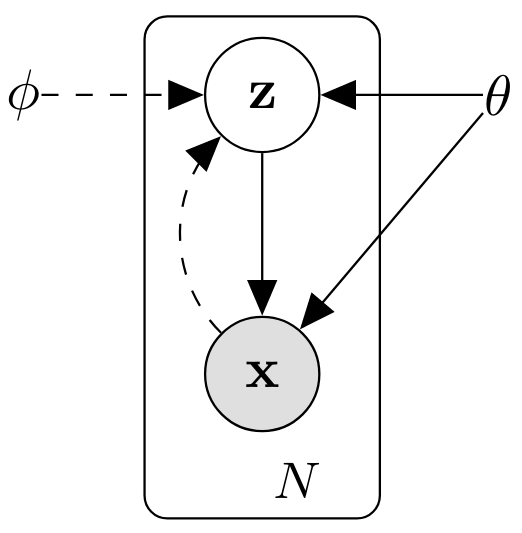
\includegraphics[width=0.25\textwidth]{images/vae-pgm.png}
	\caption
    [نمایی از مدل گرافی مورد استفاده در \vae{}.]
    {
		نمایی از مدل گرافی مورد استفاده در \vae{}. خطوط خطچین‌‌دار مربوط به تخمین توزیع پسین $p_\theta(\bff{z}|\bff{x})$ و خطوط بدون خطچین مربوط به مدل مولد
		$p_\theta(\bff{x}|\bff{z})$
		است.
		\cite{vae_text}.}
	\label{fig:vae-pgm}
\end{figure}
این ساختار به منظور یادگیری و 
\trans{استنتاج}{Inference}
مدل‌های با مدل گرافی نشان داده شده در شکل ‎\ref{fig:vae-pgm}‎ ارائه شده است. در واقع در این مدل، هر داده از یک 
\trans{متغیر نهان}{Latent Variable}
  تولید شده که \priordist{} مشخصی برای آن تعریف شده است و معمولا توزیع گاوسی نرمال است. از آنجا که محاسبه $\log p_\theta(\bff{x})$ و $\log p_\theta (z|x)$ نیازمند \inference ی 
\trans{سخت}{Intractable}
است، با بهره‌گیری از  توزیع وردشی $q_\phi(z|x)$، کران پایینی از \likelihood{} به نام \lr{ELBO} بیشینه می‌گردد.\\
از دیدگاهی دیگر، این مدل از دو بخش کلی تشکیل شده است؛ \encoder{} و \decoder{}. بخش \encoder{} وظیفه کد کردن داده ورودی در فضای نهان را داشته و در مقابل \decoder{} وظیفه برگرداندن فضای نهان به داده اصلی. تفاوت این مدل‌ها با \autoencoder{}ها در فرض و اعمال توزیع نرمال بر فضای نهان است؛ به همین دلیل امکان نمونه‌برداری از فضای نهان امکان‌پذیر خواهد بود. تابع هزینه در این ساختار، به شکل زیر تعریف شده است \cite{vae}:
\begin{equation} \label{eq:vae}
	\begin{split}
		L_{VAE} = \expected_{\bff{x} \sim p_{data}(\bff{X})} [KL(q_\phi(\bff{Z}|\bff{x}) || N(\textbf{\latin{0}},\textbf{\latin{I}}))- \expected_{\bff{z} \sim q_\phi(\bff{Z}|\bff{x})}[\log p_\theta(\bff{x}|\bff{z})]]
	\end{split}
\end{equation}
که $q_\phi(\bff{z}|\bff{x})$ تابع توزیع \encoder{} و $p_\theta(\bff{x}|\bff{z})$ تابع توزیع \decoder ست. همان طور که مشخص است، تابع هزینه از دو بخش کلی تشکیل شده است. قسمت اول وظیفه اجبار کردن تابع توزیع \encoder{} به کد کردن داده‌ها در فضای گاوسی نرمال و بخش دوم نیز وظیفه کمینه کردن خطای بازسازی داده ورودی را بر عهده دارد. بنابراین شبکه سعی در یادگرفتن مدلی دارد که علاوه بر داشتن خطای بازسازی کم، توزیع گاوسی نرمال نیز بر فضای نهان آن حاکم باشد؛ پس می‌توان بعد از آموزش مدل، با نمونه‌گیری از توزیع نرمال و کدگشایی آن توسط $p_\theta(\bff{x}|\bff{z})$ داده مصنوعی تولید نمود. از آنجا که معمولا از توزیع گاوسی نرمال به عنوان \priordist{} استفاده میگردد و خروجی \encoder{} نیز توزیعی گاوسی با ماتریس کوارایانس قطری است، عبارت $KL(q_\phi(\bff{Z}|\bff{x}) || N(\textbf{\latin{0}},\textbf{\latin{I}}))$ به صورت فرم بسته قابل محاسبه خواهد بود. نکته قابل توجه این است که طبق رابطه \ref{eq:vae}، سعی بر این است تا خروجی \encoder{} به ازای هر نقطه، مستقلا، به توزیع گاوسی نرمال نزدیک باشد؛ بنابراین این قسمت از تابع هزینه، محدودیت زیادی را بر روی خروجی \encoder{} اعمال کرده و همان طور که در آینده توضیح داده خواهد شد، فرآیند آموزش آن را در بعضی حوزه‌ها دچار مشکل می‌کند \cite{vae_text}. 
\\
\begin{figure}[H]
	\centering
	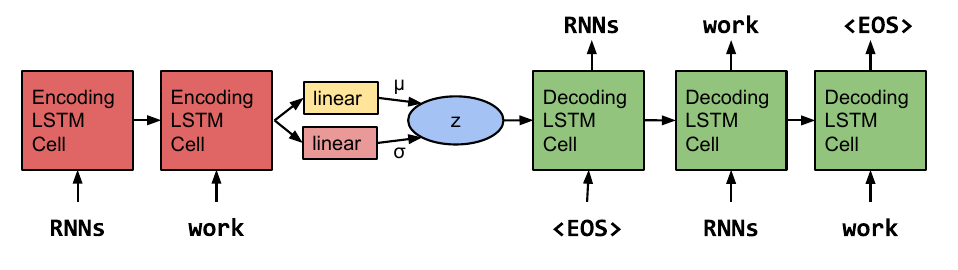
\includegraphics[width=0.5\textwidth]{images/vae-text.png}
	\caption{
		نمایی از مدل \vae{} استفاده شده در حوزه متن
		\cite{vae_text}.}
	\label{fig:vae-text}
\end{figure}
\label{chap2:latent_ignore}
آنچه که در حوزه متن اتفاق می‌افتد، صفر شدن قسمت شامل فاصله \lr{KL}  است؛ در واقع می‌توان این طور بیان کرد که کدگذار بدون توجه به معنی‌دار بودن فضای نهان، هر جمله را مستقلا به یک نقطه از فضای نهان نگاشت می‌کند. در نتیجه‌ی این روند، کدگشا هم مستقل از معنای فضای نهان جمله‌ای را تولید خواهد نمود و توزیع نرمال فرض شده بر فضای نهان یک جمله، چندان حاوی جملات مشابه آن نخواهد بود و روند آموزش به مشکل بر خواهد خورد. \\
یکی از راه‌کارهای اولیه به کار برده شده، دخیل کردن تدریجی قسمت حاوی \lr{KL} به تابع هزینه است. در واقع تابع هزینه به صورت زیر تغییر می‌کند:
\begin{equation}
	\begin{split}
		L_{VAE} = \expected_{\bff{x} \sim p_{data}(\bff{X})} [\lambda_{KL} KL(q(\bff{Z}|\bff{x}) || N(\textbf{\latin{0}},\textbf{\latin{I}}))- \expected_{\bff{z} \sim q(\bff{Z}|\bff{x})}[\log p(\bff{x}|\bff{z})]]
	\end{split}
\end{equation}
که $\lambda_{KL}$ ضریبی مثبت است. در واقع در ابتدا با قرار دادن $\lambda_{KL}=0$، مدل تنها یک خودرمزنگار ساده بوده و فضای نهان معنا داری ساخته و به مرور با میل دادن آن به یک، سعی در جمع کردن فضای نهان در فضای گاوسی نرمال خواهد داشت. جالب توجه است که چنین اتفاقی در حوزه تصویر رخ نمی‌دهد و قسمت \lr{KL} صفر نمی‌شود.
\iffalse
	این پدیده را شاید بتوان این طور توجیه کرد که از یک سو تغییرات ابتدایی فضای نهان زیاد بوده و دخیل کردن این تغییرات در تولید نمونه مورد نظر امری دشوار است؛ از سویی دیگر کدگشا به لحاظ معماری توانایی نگاشت هر نقطه از فضا را به جمله مورد نظر دارد و بنابراین رابطه تولید و استفاده از معنای فضای نهان بین کدگشا و کدگذار چندان شکل نمی‌گیرد.
\fi
گذشته از مشکلات ذکر شده، همان‌طور که در تابع هزینه آن دیده می‌شود همچنان کدگشا سعی در بالابردن درست‌نمایی داده آموزش را داشته و بنابراین این مدل همچنان مشکل \expbias{} را داشته و راه حلی برای این موضوع ارائه نمی‌کند.

به منظور رفع مشکل ذکر شده، کارهای متعددی از جهات مختلف آن را مورد بررسی قرار داده و راه حل‌هایی ارائه داده‌اند. در ادامه تعدادی از آن‌ها توضیح داده خواهند شد.
\subsubsection{عوامل صفر شدن \lr{KL}}
بررسی‌های مختلفی جهت شناسایی عوامل رخداد چنین پدیده‌ای صورت گرفته است که در ادامه به توضیح تعدادی از آن‌ها پرداخته خواهد شد.
\paragraph*{تمایل شبکه \decoder{}
	به استقلال داشتن از فضای نهان}
مقالات متعددی وجود دارند که به تحلیل \vae{} از دیدگاه نظریه اطلاعات پرداخته‌اند. یکی از این دیدگاه‌ها ارتباط روش کدینگ \bitsback{} با \vae{} است \cite{vae_lossy}.\\
فرض کنید بخواهیم اطلاعات را با استفاده از فضای نهان \vae{} کد کنیم. از آنجا که تمام اطلاعات در فضای نهان کد نشده است باید خطای بازسازی را نیز کد کنیم. بنابراین هر کد از دو بخش
$p_\bff{Z}(\bff{Z})$
(\priordist{})
و $p(\bff{X}|\bff{z})$
(توزیع \decoder{})
تشکیل خواهد و میانگین طول کد به شرح زیر است:
\begin{gather}
	\mathcal{L}_{naive} = \expected_{\bff{x} \sim \text{data}, \bff{z} \sim q(\bff{Z}|\bff{x})} [-\log p(\bff{z}) - \log p(\bff{x}|\bff{z})]
\end{gather}
می‌توان روش کدینگ فوق را با استفاده از اطلاعات $q(\bff{z}|\bff{x})$ بهبود داد؛ چراکه این توزیع به طور میانگین حداکثر $H(q(\bff{Z}|\bff{x}))$ اطلاعات در خود دارد. روش به این صورت خواهد بود که \decoder{} هنگام بازگشایی کد، به توزیع تخمینی $\prob(\bff{z}|\bff{x})$ که فرستنده از آن استفاده می‌کند، دسترسی داشته و در نتیجه به اندازه $\log q(\bff{z}|\bff{x})$ از طول کد کم خواهد شد. میانگین طول کد به صورت زیر تغییر خواهد کرد \cite{vae_lossy}.
\begin{gather}
	\mathcal{L}_{\text{BitsBack}} = \expected_{\bff{x} \sim \text{data}, \bff{z} \sim q(\bff{Z}|\bff{x})} [\log q(\bff{z}|\bff{x}) -\log p(\bff{z}) - \log p(\bff{x}|\bff{z})]
\end{gather}
که برابر با تابع هزینه \vae{} است \cite{vae_lossy}:
\begin{gather}
	\begin{align}
		\mathcal{L}_{\text{BitsBack}} = & \expected_{\bff{x} \sim \text{data}} \Big[\expected_{\bff{z} \sim q(\bff{Z}|\bff{x})} [\log p(\bff{x}|\bff{z})] + KL\big(q(\bff{Z}|\bff{x}) ~||~ p(\bff{Z})\big)\Big] \nonumber
		\\
		=                               & \mathcal{L}_{\text{VAE}}
	\end{align}
\end{gather}
از سوی دیگر می‌توان کران پایینی برای تابع هزینه فوق بدست آورد که تابعی از آنتروپی توزیع داده اصلیست. می‌دانیم کران پایین میانگین طول کد برای کد کردن یک نوع داده، آنتروپی آن است. طبق روابط چنین بدست می‌آید \cite{vae_lossy}:
\begin{align}
	\mathcal{L}_{\text{BitsBack}} =
	                                                                           & \expected_{\bff{x} \sim \text{data}, \bff{z} \sim q(\bff{Z}|\bff{x})} [\log q(\bff{z}|\bff{x}) -\log p(\bff{z}) - \log p(\bff{x}|\bff{z})] \nonumber
	\\
	=
	                                                                           & \expected_{\bff{x} \sim \text{data}} [-\log p(\bff{x}) + KL\big(q(\bff{Z}|\bff{x}) ~||~ p(\bff{Z}|\bff{x})\big)] \nonumber
	\\
	\xrightarrow[\text{\lr{by Shannon entropy}}]{\text{\lr{lower bound}}} \geq & \expected_{\bff{x} \sim \text{data}} [-\log p_{\text{data}}(\bff{x}) + KL\big(q(\bff{Z}|\bff{x}) ~||~ p(\bff{Z}|\bff{x})\big)] \nonumber
	\\
	=
	                                                                           & \mathcal{H}(\text{data}) + \expected_{\bff{x} \sim \text{data}} [KL\big(q(\bff{Z}|\bff{x}) ~||~ p(\bff{Z}|\bff{x})\big)]
\end{align}
بنابراین این روش کدینگ به اندازه
$KL\big(q(\bff{Z}|\bff{x}) ~||~ p(\bff{Z}|\bff{x})\big)$
از کدینگ بهینه فاصله دارد و هر قدر این فاصله کمینه گردد، کدینگ نیز طبیعتا بهینه‌تر خواهد بود. \\
اما رابطه فوق چه کمکی به تحلیل پدیده صفر شدن \lr{KL} می‌کند؟ فرض کنید که \decoder{}
($p(\bff{x}|\bff{z})$)
تابعی با قدرت مدل‌سازی بینهایت بوده و توانایی مدل کردن $p_{\text{data}}(\bff{x})$ را مستقل از $\bff{z}$ دارد. از سوی دیگر این امکان برای $q(\bff{z}|\bff{x})$ وجود دارد تا بر خلاف خواسته ما، ضمن عدم استفاده مفید از $\bff{x}$ توزیعی صرفا برابر با $p(\bff{z})$ بسازد. در نتیجه می‌توان با این گونه مدلسازی با آنکه نه $q$ اطلاعات مفیدی را کد کرده و نه $p(\bff{x}|\bff{z})$ از فضای نهان به درستی استفاده می‌کند، از هزینه اضافی
$KL\big(q(\bff{Z}|\bff{x}) ~||~ p(\bff{Z}|\bff{x})\big)$
جلوگیری کرده و به کدینگ بهینه نزدیک شد. این سناریو دقیقا همان اتفاقی است که احتمال وقوع آن در هنگام استفاده از \decoder{} با ساختار \autoregressive{} وجود دارد. برای مثال در صورت استفاده از ساختار \lstm{} (که در تئوری توانایی مدل کردن هر توزیعی را دارد)، \decoder{} می‌تواند بدون استفاده از فضای نهان، توزیع داده اصلی را مدل کند و در نتیجه رابطه موثری بین \decoder{} و \encoder{} شکل نگرفته و 
$KL\big(q(\bff{Z}|\bff{x}) ~||~ p(\bff{Z}|\bff{x})\big)$
صفر شود. به عنوان یک گزاره کلی چنین می‌توان گفت که \decoder{} به اندازه‌ای که بتواند، اطلاعات داده را به صورت محلی مدل کند این کار را انجام داده و هر آنچه که امکان مدلسازی آن به صورت محلی نباشد و یا به عبارت دیگر مربوط به ویژگی‌های کلی یک نمونه باشد، در فضای نهان کد نموده و از آن استفاده می‌کند \cite{vae_lossy}.
\\
با استفاده از تحلیل فوق می‌توان به این نتیجه رسید که چون \vae{} با معماری 
\trans{شبکه‌های عصبی پیچشی}{Convolutional Neural Networks (CNN)}
 در حوزه تصویر، ساختاری  غیر \autoregressive{} دارد، بدون استفاده از فضای نهان، چندان توانایی کم کردن خطای بازسازی را نداشته و مجبور به استفاده از فضای نهان خواهد بود؛ در نتیجه مشکلی که در مدل‌های متنی به وجود می‌آید، در حوزه تصویر با این معماری گزارش نشده است. به طور کلی هر مقدار معماری مورد استفاده توانایی مدل‌سازی محلی کمتری داشته باشد، کمتر مشکل وجود خواهد داشت. توانایی مدل‌سازی محلی را در معماری \cnn{} می‌توان به کم کردن \receiptivefield{} و در \lstm{} به حذف بعضی از کلمات ورودی تعبیر نمود \cite{vae_lossy, vae_dialated, vae_hybrid}.
\paragraph*{بهینه‌های سراسری نامطلوب}
همان ‌طور که در بخش قبل توضیح داده شد، با تطبیق دادن روش کدینگ  \lr{Bits-Back} با مدل \vae{}، می‌توان به این نتیجه رسید که \decoder{} برای رسیدن به میانگین طول کد کمینه، تمایل به استفاده نکردن از فضای نهان دارد. علاوه بر این موضوع، می‌توان نقاطی را یافت که \lr{ELBO} کمینه گردد و از فضای نهان نیز استفاده نگردد \cite{infovae}. می‌دانیم رابطه زیر برای \lr{ELBO} برقرار است:
\begin{align}
	\mathcal{L}_{\text{ELBO}} = & \expected_{\bff{x} \sim p_\text{data}, \bff{z} \sim q(\bff{Z}|\bff{x})} [- \log p_\theta(\bff{x}|\bff{z}) + KL\big(q_\phi(\bff{Z}|\bff{x}) ~ || ~ p(\bff{Z})\big)] \nonumber
	\\
	=                           & \expected_{\bff{x} \sim p_\text{data}} [-\log p_\theta(\bff{x}) + KL\big(q_\phi(\bff{Z}|\bff{x}) ~||~ p_\theta(\bff{Z}|\bff{x})\big)] \nonumber
\end{align}

فرض کنید $p_\theta(\bff{x}|\bff{z})$ وجود داشته باشد که بتواند توزیع داده اصلی را یاد بگیرد؛ به عبارت دیگر، $\theta$ای وجود داشته باشد که $p_\theta(\bff{x}|\bff{z}) = p^*(\bff{x})$. با داشتن این فرض،
$p_\theta(\bff{x}) = p^*(\bff{x})$
و
$p_\theta(\bff{z}|\bff{x})$
برابر با \priordist{} خواهد شد \cite{infovae}:
\begin{gather}
	p_\theta(\bff{X}) = \int_\bff{z} p(\bff{z}) p_\theta(\bff{X}|\bff{z})  = \int_\bff{z} p(\bff{z}) p^*(\bff{X}) = p^*(\bff{X}) \int_\bff{z} p(\bff{z}) = p^*(\bff{X})
	\\
	p_\theta(\bff{Z}|\bff{x}) = \frac{p_\theta(\bff{x}|\bff{Z}) p(\bff{Z})}{p_\theta(\bff{x})} = \frac{p^*(\bff{x}) p(\bff{Z})}{p^*(\bff{x})} = p(\bff{Z})
\end{gather}
حال $q_\phi(\bff{z})$ می‌تواند به سمت $p(\bff{z})$ رفته تا عبارت \lr{KL} بین \posterior{} واقعی و تخمینی صفر گردد. از سوی دیگر هم \likelihood{} بیشینه مقدار خود را دارد ($p_\theta(\bff{x}) = p^*(\bff{x})$) و در نتیجه این حالت یک حالت بهینه سراسری است. از آنجا که $q_\phi(\bff{z}|\bff{x})$ به $p(\bff{z})$ تبدیل شده است، بنابراین رابطه‌ای بین $\bff{x}$ و $\bff{z}$ تحت $q_\phi(\bff{z}|\bff{x})$ وجود نداشته و به عبارت دیگر فضای نهان معنای مطلوب را نداشته گرچه که به بهینه سراسری رسیده‌ایم \cite{infovae}.
\paragraph*{عقب ماندن شبکه
	\encoder{}
	در تخمین توزیع پسین واقعی}
از زاویه‌ای دیگر نیز می‌توان این پدیده را مورد بررسی قرار داد. فروپاشی توزیع \posterior{} به زبان ریاضی به حالتی از مدل اطلاق می‌گردد که
$q_\phi(\bff{z}|\bff{x}) = p_\theta (\bff{z}|\bff{x}) = p(\bff{z})$
است \cite{vae_lagging}. این حالت را می‌توان به دو زیر حالت تقسیم کرد؛ حالت $p_\theta(\bff{z}|\bff{x}) = p(\bff{z})$ و حالت $q_\phi(\bff{z}|\bff{x}) = p(\bff{z})$ که آن‌ها را به ترتیب فروپاشی مدل و فروپاشی استنتاج می‌نامیم. با توجه به این تقسیم بندی می‌توان آزمایشی را ترتیب داد تا متوجه شد کدام حالت موجب چنین رخدادی می‌گردد. به این منظور میانگین دو توزیع $p_\theta(\bff{z}|\bff{x})$ و $q_\phi(\bff{z}|\bff{x})$ که به ترتیب با $\mu_{\bff{x},\theta}$ و $\mu_{\bff{x},\phi}$ نمایش داده می‌شوند را در حین آموزش بررسی و رسم می‌کنیم. هر نقطه $x$ با استفاده از توزیع‌های حاصل از شبکه‌های \encoder{} و \decoder{} به فضای
$(\mu_{\bff{x},\phi}, \mu_{\bff{x},\theta})$
برده شده و سپس نموداری به شکل زیر رسم می‌گردد:
\begin{figure}[H]
	\centering
	\includegraphics[width=0.5\textwidth]{images/lagging1.pdf}
	\caption
    [نموداری بر فضای میانگین توزیع پسین $(\mu_{x,\phi}, \mu_{x,\theta})$.]
    {
		نموداری بر فضای میانگین توزیع پسین $(\mu_{x,\phi}, \mu_{x,\theta})$. محور افقی میانگین توزیع \posterior{} مدل و محور عمودی میانگین توزیع \posterior{} تخمینی را نشان می‌دهد. خط چین قطری نیز حالتی را نشان می‌دهد که میانگین توزیع \posterior{} مدل (واقعی) با تخمینی یکسان شده است \cite{infovae}.
	}
\end{figure}

از آنجا که میانگین \priordist{} برابر صفر است، بنابراین اگر $\mu_{\bff{x},\phi} = 0$ شود فروپاشی استنتاج و اگر $\mu_{\bff{x},\theta} = 0$ باشد فروپاشی مدل اتفاق افتاده است \cite{infovae}. لازم به ذکر است که بایستی ابعاد $\bff{z}$ به گونه‌ای باشد تا بتوان آن را به صورت کارا محاسبه کرد؛ ازین رو $\bff{z}$ یک عدد یک بعدی در نظر گرفته شده است. محور قطری نیز مربوط به حالتی است که $p_\theta(\bff{z}|\bff{x})$ و $q_\phi(\bff{z}|\bff{x})$ از نظر میانگین بر یکدیگر منطبق بوده و توزیع پسین تخمینی، کار خود را به درستی انجام داده است. مبدا نیز مربوط به حالت بهینه محلیِ فروپاشی \posteriordist{} است؛ این در حالی است که احتمالا نقاط بهینه محلی مطلوب‌تر جایی بر روی محور قطری و در اطراف مبدا خواهند داشت.
نمودار‌های زیر حاصل انجام این آزمایش در روند آموزش است.

\begin{figure}[H]
	\centering
	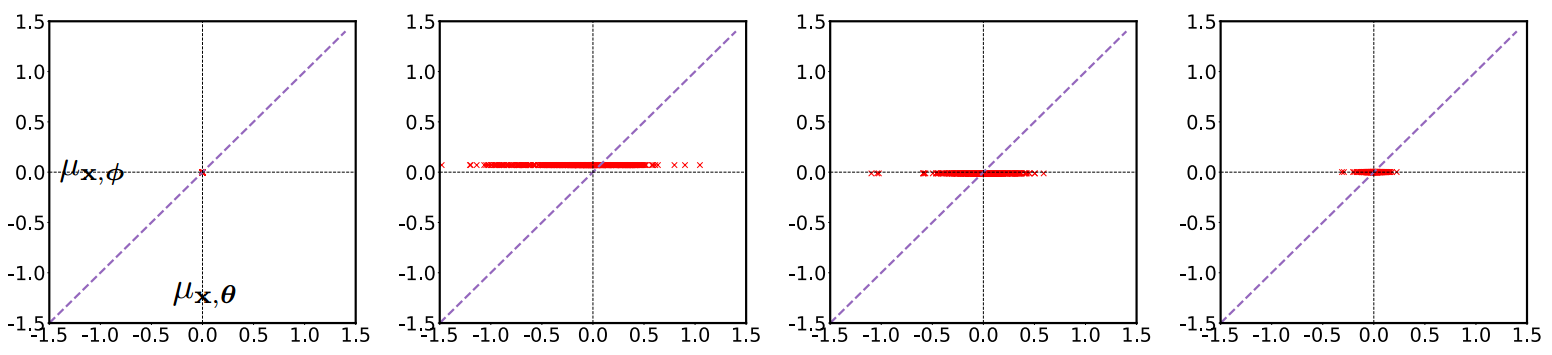
\includegraphics[width=1.\textwidth]{images/lagging2.png}
	\caption
    [مشاهده‌ای از نحوه رخداد حالت فروپاشی استنتاج]
    {
        مشاهده‌ای از نحوه رخداد حالت فروپاشی استنتاج. نمودارهای فوق از تصویر کردن ۵۰۰ نقطه از داده اصلی بر فضای نهان (در ۴ مقطع زمانی. به ترتیب از شکل سمت چپ به راست، گام آموزشی ۰ ام، ۲۰۰ ام، ۲۰۰۰ ام و انتهایی) بدست آمده است. آنچه که در تصویر فوق مشخص است، آن است که در ابتدای آموزش، دو متغیر $\bff{z}$ و $\bff{x}$ از یکدیگر مستقل بوده و در روند آموزش نیز شبکه \encoder{} تخمین صحیحی از \posteriordist{} نداشته و در نتیجه باعث ایجاد حالت فروپاشی استنتاج می‌شود.
	}
\end{figure}
آن طور که از تصاویر برداشت می‌شود به این صورت است که ابتدا نقاط به صورت متمرکز در مبدا جمع شده‌اند اما در ادامه، نقاط در محور افقی گسترده شده‌اند و در انتها مجددا به سمت متمرکز شدن پیش رفته اند. نکته قابل توجه این است که در تمامی این حالات نقاط در محور افقی پراکنده شده‌اند \cite{infovae}. برای توجیه این مشاهده می‌توان از صورت دیگری از رابطه \lr{ELBO} بهره برد. می‌دانیم \lr{ELBO} برابر با عبارت زیر است \cite{vae, vae_lagging}:
\begin{gather}
	\mathcal{L}_{\text{ELBO}}(\bff{x};\theta, \phi) = \log p_\theta(\bff{x}) - {KL}(q_\phi(\bff{Z}|\bff{x})~||~ p_\theta(\bff{Z}|\bff{x}))
\end{gather}
که عبارت اول مربوط به \likelihood{} حاشیه‌ای و عبارت دوم مربوط به فاصله توزیع تخمینی $q_\phi(\bff{z}|\bff{x})$ از توزیع پسین واقعی مدل ($p_\theta(\bff{z}|\bff{x})$) است. واضح است که پارامتر $\phi$ تنها تحت تاثیر عامل \lr{KL} بوده در حالی که پارامتر $\theta$ علاوه بر این، تحت تاثیر عبارت \likelihood{} حاشیه‌ای نیز هست. علاوه بر این تنها عاملی که باعث ایجاد رابطه بین $\bff{x}$ و $\bff{z}$ می‌گردد،
\likelihood{}
است و بخش دوم تنها سعی در نزدیک کردن دو توزیع $p_\theta(\bff{z}|\bff{x})$ و $q_\phi(\bff{z}|\bff{x})$ دارد \cite{infovae}.

حال با نگاه داشتن به رابطه فوق، این پدیده را این طور می‌توان تفسیر نمود که با وجود اینکه ابتدا فضای نهان ساخته شده تقریبا مستقل از فضای داده‌های ورودی است، با پراکنده شدن نقاط به صورت افقی در ادامه روند آموزش، رابطه‌ای بین $\bff{z}$ و $\bff{x}$ تحت مدل $p_\theta(\bff{x})$ در حال شکل‌گیری است؛ اما به دلیل اینکه شبکه \encoder{} به هیچ عنوان تخمین صحیحی از \posteriordist{} واقعی ندارد و همزمان در حال کمینه کردن هر دو قسمت عبارت \lr{ELBO} نسبت به پارامترهای هر دو شبکه‌ی \encoder{} و \decoder{} هستیم، در نتیجه با ادامه آموزش، رابطه بین این دو متغیر به مرور بر اثر غلبه بخش حاوی فاصله \lr{KL} بر بخش \likelihood{} حاشیه‌ای، از دست رفته و سیستم دچار یک بهینه محلی می‌گردد \cite{infovae}.

\subsection{مدل‌های ارائه شده برای رفع مشکل صفر شدن \lr{KL}}
به طور کلی راه حل‌های ارائه شده یا از جنس تغییر معماری ‎\decoder{}‎ و ضعیف کردن قدرت ‎\autoregressive{}‎ آن، تغییر ‎\priordist{}‎ و یا تغییر تابع هزینه هستند. در ادامه به توضیح برخی از این روش‌ها پرداخته خواهد شد.
\subsubsection{استفاده از \cnn{} به جای \lstm{} در \decoder{}}
\begin{figure}[h]
	\centering
	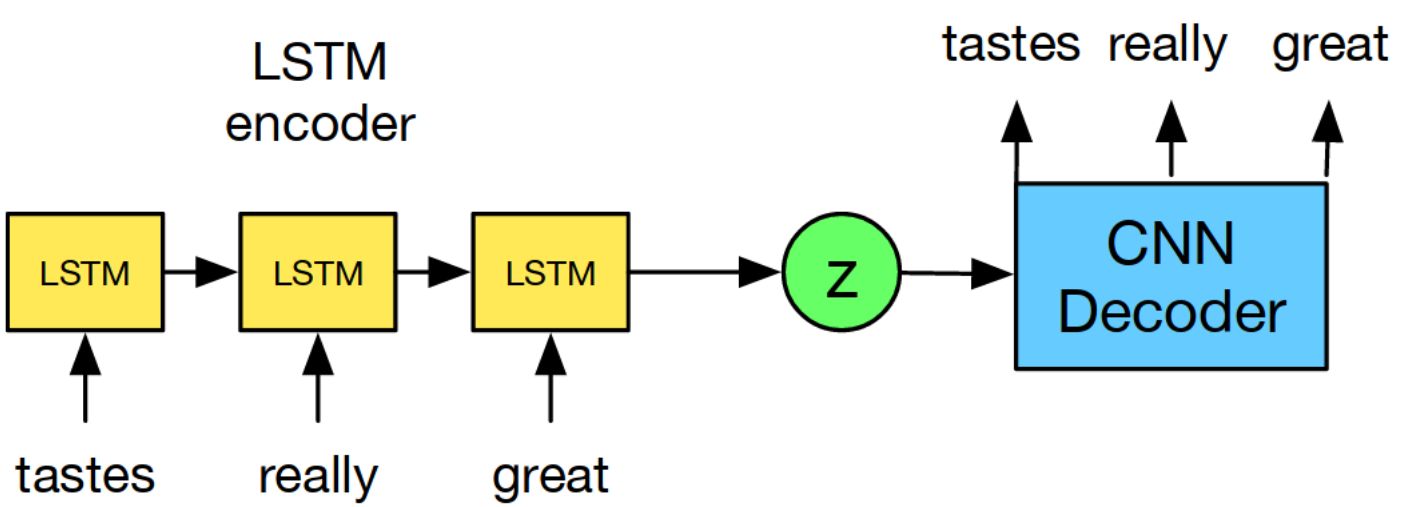
\includegraphics[width=0.5\textwidth]{images/dialated-conv1.png}

	\vspace{0.5cm}

	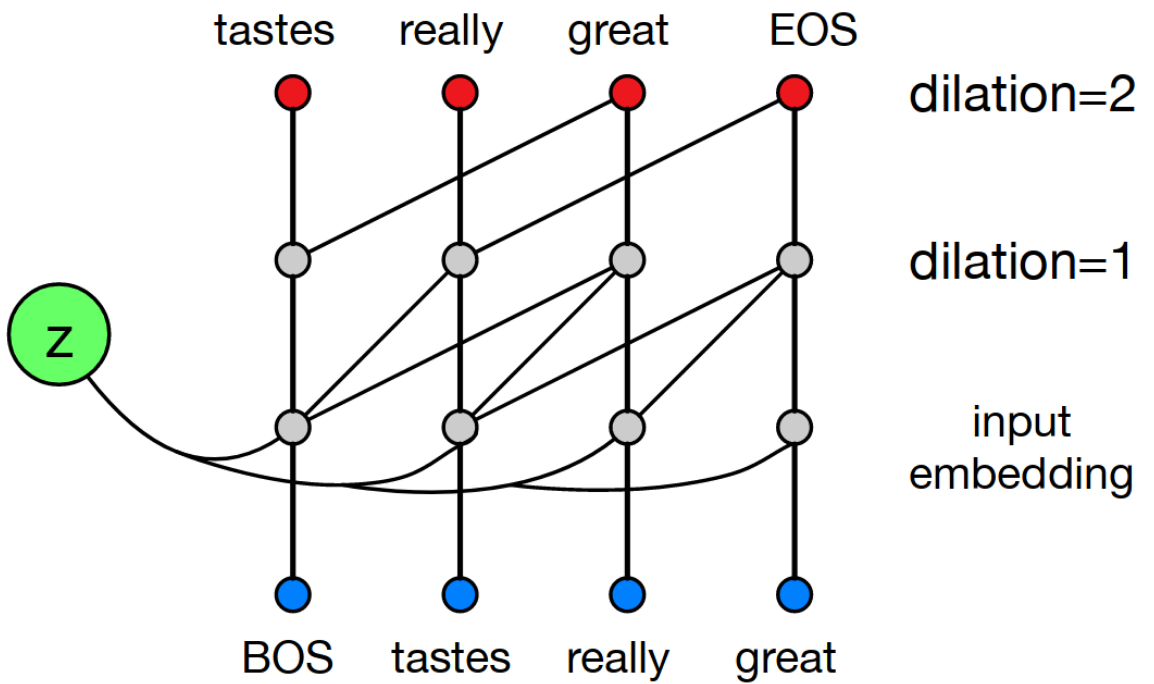
\includegraphics[width=0.5\textwidth]{images/dialated-conv2.png}
	\caption{
		معماری کلی شبکه ارائه شده که از \cnn{}  با کانولوشن‌های \dilated{} در  ‎\decoder{}‎ بهره می‌برد.
	}
	\label{fig:dialted_conv}
\end{figure}
راه حل‌های اولیه بیشتر در حوزه تغییر ساختار ‎\decoder{}‎ هستند. دلیل چنین رویکردی در این بود که می‌توان مشکل را در قدرت زیاد مدل‌های ‎\lstm{} در مدلسازی به صورت ‎\autoregressive{}‎ جست و جو کرد \cite{vae_dialated}؛ چراکه در حوزه تصویر که هر پیکسل مستقل از سایر پیکسل‌ها تولید می‌گردد، چنین پدیده‌ای گزارش نشده است. بنابراین یک راه حل استفاده از مدل‌هایی است که قدرت \autoregressive{} کمتری دارند. برای مثال همان طور که در شکل ‎\ref{fig:dialted_conv}‎ نشان داده شده است، می‌توان ‎\decoder{}‎ را با وام گرفتن از ایده شبکه ‎\lr{PixelCNN}‎ با معماری ‎\cnn{}‎ پیاده‌سازی و جایگزین ‎\lstm{}‎ نمود. به طور دقیق‌تر برای پیشبینی هر پیکسل، پیکسل‌های پیش‌رو پوشانده شده، از فیلتر‌های یک بعدی و اتصالات
\trans{انبساطی}{Dilated}
در کانولوشن‌ها بهره گرفته شده که در نتیجه
\trans{حوزه تاثیر}{Receiptive field}
در هر لایه نسبت به لایه قبل، افزایش نمایی پیدا کند \cite{vae_dialated}. در واقع با زیاد شدن تعداد لایه‌های با کانولوشن‌های \dilated{}، 
\trans{زمینه}{Context}
 طولانی‌تری در خروجی یک گره از لایه مورد نظر دخیل خواهد شد. برای مثال اگر ضریب انبساط ۲ استفاده گردد، \receiptivefield{}‎ در هر لایه نسبت به لایه قبل تقریبا دو برابر شده و در نتیجه از آنجا که می‌بایست کلمه آخر جمله تابعی از تمام کلمات پیشین باشد،‌ نیاز به $‎\log T$ لایه خواهد بود که $T$ طول بلندترین جمله است. ادعای مقاله بر اساس آزمایش‌های متفاوت بر این است که ساختار \cnn{} بیشتر متکی بر فضای نهان  $Z$ بوده و بنابراین مشکل ذکر شده را مقداری تقلیل می‌دهد. نکته قابل ذکر این است که در این حالت نیز اگر ‎اندازه شبکه بسیار بزرگ شود مجددا مشکل صفر شدن ‎\lr{KL}‎ ظهور پیدا می‌کند \cite{vae_dialated}.

\subsubsection{\aae{}
    \protect\LTRfootnote{Adversarial autoencoder (AAE)}
} \label{sec:aae}
مدل \aae{}، نسخه تغییر یافته‌ای از مدل \vae{} است تا بخشی از ضعف‌های آن را بپوشاند. همان طور که قبلا نیز توضیح داده شد، تابع هزینه \vae{} از دو بخش تشکیل شده است. بخش اول مربوط به کمینه کردن خطای بازسازی و بخش دوم مربوط به سوق دادن فضای نهان به توزیع گاوسی نرمال است. مدل \aae{}، با حفظ بخش مربوط به خطای بازسازی، در بخش دوم به جای نزدیک کردن توزیع خروجی ‎\encoder{}‎ به  ‎‎\priordist{‎}‎
($q(\bff{z}|\bff{x}) ‎\leftrightarrow p(\bff{z})$)،
سعی در نزدیک کردن توزیع 
\trans{حاشیه‌ای}{Marginal}
خروجی  ‎\encoder{‎}‎  را  به \priordist{} مورد نظر دارد
($q(z) ‎\leftrightarrow  p(z)$) \cite{aae}.
در واقع توزیع \marginal{} $q(\bff{z})$ به صورت زیر تعریف می‌شود:
\begin{gather}
	q(Z) = \sum_\bff{x} p_{data}(\bff{x}) q(\bff{Z}|\bff{x})
\end{gather}
و هدف نزدیک کردن توزیع $q(\bff{z})$ به $p(\bff{z})$ خواهد بود \cite{aae}. بنابراین در مقایسه با مدل \vae{}، اجازه داده می‌شود تا به جای اینکه خروجی \encoder{} به ازای هر نمونه، مستقل از سایر نمونه‌ها به یک توزیع گاوسی نرمال نزدیک شود، توزیع ‎\marginal{}‎ نمونه‌های داده واقعی در فضای نهان، یک توزیع نرمال گاوسی باشد.
\begin{figure}[H]
	\centering
	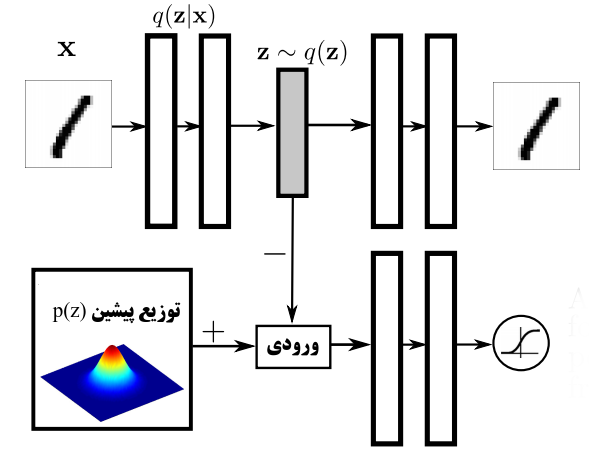
\includegraphics[width=.6\textwidth]{images/aae.png}
	\caption
    [نمایی از مدل  \aae{}.]
    {
		نمایی از مدل  \aae{}. در واقع این مدل، همان مدل \autoencoder{} است که بخش منظم‌ساز مربوط به نزدیک کردن $q(\bff{z})$ به $p(\bff{z})$ به آن افزوده شده است \cite{aae}. برای نزدیک کردن این دو توزیع نیز از رویکرد \gan{} استفاده شده که نمونه‌های \priordist{} نمونه‌های مثبت و نمونه‌های تولید شده توسط \encoder{} نمونه‌های منفی تلقی شده و داده ورودی شبکه \discriminator{} می‌سازند.
	}
	\label{fig:aae}
\end{figure}
گفته شد که بایستی دو توزیع $p(\bff{z})$ و $q(\bff{z})$ به یکدیگر نزدیک شوند. حال بر خلاف آنچه که در مدل \vae{} اتفاق می‌افتاد که بخش $KL$ نیاز به محاسبه به صورت فرم بسته داشت، با وام‌گیری از ایده \gan{}، می‌توان \discriminator ‌ای آموزش داد تا نمونه‌های \priordist{} را از نمونه‌های توزیع \marginal
$q(\bff{z})$
جدا کند. در واقع اگر بخواهیم با ادبیات شبکه‌های تخاصمی معادل‌سازی کنیم، مولد $q(\bff{z})$ و توزیع داده واقعی $p(\bff{z})$ خواهد بود که نمایی از این روش نیز در شکل \ref{fig:aae} آمده است. رابطه تابع هزینه این مدل به شکل زیر است \cite{aae}:
\begin{gather}
	L_{AAE}(\phi, \theta) =
	- \expected_{\bff{x} \sim p_{data}, \bff{z} \sim q_\phi(\bff{Z}|\bff{x})} [\log (D(\bff{z}))]
	+ \expected_{\bff{x} \sim p_{data}, \bff{z} \sim q_\phi(\bff{Z}|\bff{x})}[\log p_\theta(\bff{x}|\bff{z})]\\
	L_{AAE}(D) =
	- \expected_{\bff{z} \sim p(\bff{Z})} [\log D(\bff{z})]
	- \expected_{\bff{x} \sim p_{data},\bff{z} \sim q_\phi(\bff{Z}|\bff{x})} [\log (1 - D(\bff{z}))]
\end{gather}
که $q_\phi(\bff{z}|\bff{x})$ توزیع \encoder{}،
$p_\theta(\bff{x}|\bff{z})$
توزیع \decoder{} و $p(\bff{z})$ توزیع پیشین است. روند بهینه‌سازی به این صورت است که مانند \gan{} از دو بخش تشکیل شده است؛ بخش بهینه‌سازی خطای بازسازی و بخش تخاصمی. در بخش خطای بازسازی، تنها \autoencoder{} به منظور کاهش خطای بازسازی آموزش داده می‌شود و در بخش تخاصمی، ابتدا \discriminator{} به منظور جداسازی نمونه‌های واقعی از مصنوعی و سپس \encoder{} به منظور نزدیک کردن توزیع \marginal{}‎ فضای نهان به \priordist{} آموزش داده می‌شود \cite{aae}.\\
نکته دیگری که می‌توان در نحوه آموزش مدل به آن اشاره نمود این است که کافیست تا بتوانیم از دو توزیع پیشین و حاشیه‌ای \encoder{} نمونه‌برداری کنیم و مانند مدل \vae{}، نیازی به داشتن فرم بسته رابطه بالا نیست که از مزیت‌های این مدل به شمار می‌رود؛ اما از سوی دیگر این مدل بدون پشتوانه نظری و بررسی رابطه آن با \likelihood{} ارائه شد.\\
در مورد نحوه عملکرد ‎\encoder{}‎ چندین گزینه وجود دارد:
\begin{itemize}
	\item \textbf{\deterministic{}:}
	      در اینجا، $q(\bff{z}|\bff{x})$ یک تابع قطعی از $x$ بوده و تنها عامل تصادفی بودن توزیع  $q(\bff{z})$، توزیع داده واقعی $p_{data}‎(\bff{x})$ است \cite{aae}.
	\item \textbf{توزیع \posterior{} گاوسی:}
	      می‌توان خروجی ‎\encoder{}‎ را توزیع گاوسی با ماتریس کوواریانس قطری در نظر گرفت. بنابراین دو عامل تصادفی در $q(\bff{z})$ وجود خواهد داشت؛ توزیع داده اصلی و توزیع خروجی ‎\encoder{}‎ . به منظور آموزش مدل مشکلات مشابه آموزش ‎\vae{}‎ وجود دارد که مجددا می‌توان از ترفند ‎\reparametrization{}‎ بهره برد \cite{aae}.
	\item \textbf{
        \trans{تخمین‌گر عمومی}{Universal approximator}
         توزیع \posterior{}:}
	      این حالت، کلی‌ترین حالت ممکن برای ‎‎\encoder{}‎ است. ‎\encoder{}‎ به این صورت عمل می‌کند که با گرفتن نویز $‎‎\eta$ (با داشتن توزیع از قبل تعریف شده) و نمونه $\bff{x}$، یک $\bff{z}$ در فضای نهان تولید می‌کند. در واقع ‎\encoder{}‎ یک تابع قطعی از $\bff{x}$ و $‎\eta$ است. مانند حالت قبل، دو عامل تصادفی وجود دارد؛ توزیع داده اصلی و توزیع نویز اولیه. اما بر خلاف مدل قبل، خروجی ‎\encoder{}‎ ، توزیع از پیش تعیین شده‌ای نداشته و با پارامترهای ‎شبکه \encoder{}‎ پارمتری می‌شود. در این حالت $q(\bff{z})$ به شکل زیر خواهد بود:
	      \begin{gather}
		      q(\bff{z}) = \sum_\bff{x} q(\bff{z}|\bff{x}) p_{data}(\bff{x}) = \sum_\bff{x} \sum_\eta p_{data}(\bff{x}) p(\eta)  q(\bff{z}|\bff{x}, \eta)
	      \end{gather}
\end{itemize}
لازم به ذکر است که در دو حالت آخر، ‎با داشتن دو عامل تصادفی، احتمالا توزیع  ‎\marginal{}‎ ‎\encoder{}‎ ، توزیعی با تغییرات  نَرم‌تر خواهد بود \cite{aae}.
\subsubsection{\wae} \label{chap2:wae}
مدل \wae{} که در ادامه معرفی خواهد شد، نسخه عمومی‌تر مدل \aae{}‎ بوده که به لحاظ تئوری نیز بررسی گردیده است.\\
در بخش ‎\ref{sec:aae}‎ توضیح داده شد که تفاوت ‎\aae{}‎ با مدل ‎\vae{}‎، در نحوه اعمال توزیع مورد نظر بر فضای نهان است. با تکیه بر همین نکته، حالت کلی‌تری از ‎\aae{}‎ به نام ‎\wae{}‎ ارائه شد. در واقع همان طور که در شکل ‎‎\ref{fig:wae}‎ مشخص است، در ‎\vae{}‎ توزیع خروجی \encoder{} به ازای هر نمونه به ‎\priordist{}‎ نزدیک می‌شود. در نتیجه این عمل، خروجی \encoder{} به ازای نمونه‌های متفاوت مجبور به داشتن همپوشانی خواهد شد؛ بنابراین بازسازی نمونه‌های داده اصلی از فضای نهان با مشکل مواجه خواهد شد. در مقابل، در ‎\wae{}‎ مقداری دست مدل در نحوه اعمال ‎‎\priordist{}‎ به فضای نهان باز بوده و تنها کافیست توزیع ‎\marginal{}‎ حاکم بر فضای نهان دارای ‎\priordist{}‎ باشد \cite{wae}.\\
\begin{figure}[H]
	\centering
	\begin{subfigure}[b]{0.4\textwidth}
		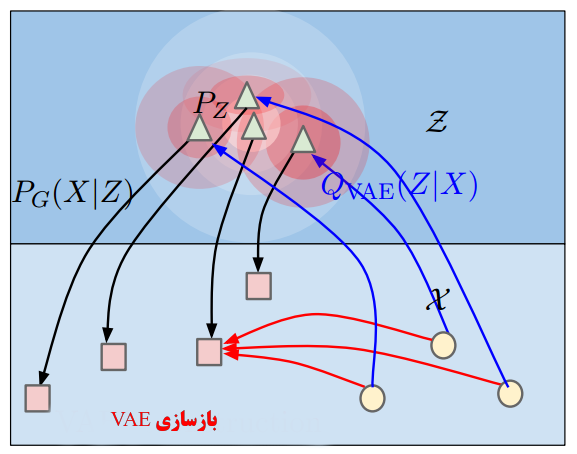
\includegraphics[width=\textwidth]{images/wae1.png}
		\caption{\vae}
		\label{fig:wae-vae}
	\end{subfigure}
	\begin{subfigure}[b]{0.4\textwidth}
		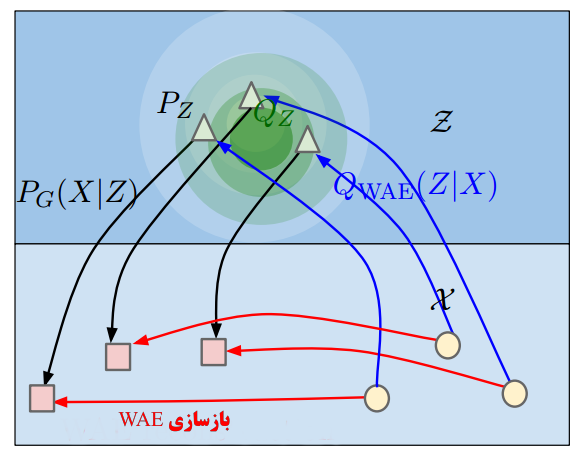
\includegraphics[width=\textwidth]{images/wae2.png}
		\caption{\wae}
		\label{fig:wae-wae}
	\end{subfigure}
	\caption
    [مقایسه نحوه بازسازی در مدل  ‎‎\wae{}‎ با ‎\vae{}‎.]
    {
		مقایسه نحوه بازسازی در مدل  ‎‎\wae{}‎ با ‎\vae{}‎. دوایر قرمز رنگ در فضای نهان مربوط به توزیع (گاوسی) خروجی ‎\encoder{}‎، دوایر سبز رنگ مربوط به توزیع ‎‎\marginal{}‎ خروجی ‎\encoder{}‎ و  دوایر سفید رنگ، متناظر با ‎\priordist{}‎ (گاوسی نرمال) است. همان طور که در شکل ‎\subref{fig:wae-vae}‎ مشخص است، هر ناحیه قرمز سعی در نزدیک شدن به ناحیه سفید رنگ دارد؛ بنابراین به دلیل وجود همپوشانی بین نواحی مختلف قرمز، مشکلاتی در بازسازی پیش خواهد آمد. این در حالیست که در مدل ‎\wae{}‎ ، تمرکز بر اعمال توزیع گاوسی بر توزیع ‎\marginal{}‎ \encoder{}‎‎ است \cite{wae}.
	}
	\label{fig:wae}
\end{figure}
بر خلاف آن که در روش ‎\aae{}‎ اظهار نظری راجع به رابطه تابع هزینه معرفی شده و ‎\likelihood{}‎ مدل ارائه نشد، مدل ‎\wae{}‎ به بررسی این موضوع پرداخته است.
مدل گرافی در نظر گرفته شده برای این روش مانند مدل گرافی ‎\vae{}‎ است. متغیر نهان $\bff{z}$ ای با توزیعی مشخص و ثابت وجود دارد که نمونه $\bff{x}$ از آن بدست خواهد آمد. اگر ‎\priordist{}‎ متغیر نهان را با $p_\bff{Z}(\bff{z})$ و ‎توزیع ‎‎‎\decoder{}‎‎ را با $p_G(\bff{x}|\bff{z})$ نشان دهیم، توزیع ‎\marginal{}‎
$p_G(\bff{x})$
به صورت زیر تعریف می‌شود:
\begin{gather}
	p_G(\bff{X}) = \sum_\bff{z} p_\bff{Z}(\bff{z}) p_G(\bff{X}|\bff{z})
\end{gather}
حال برای اینکه این توزیع را به توزیع $p_{data}‎(\bff{x})$ نزدیک کنیم، از فاصله‌های متعددی می‌توان استفاده نمود \cite{wae}. در اینجا همان طور که از نام مدل بر‌می‌آید، از فاصله ‎‎ \wasser{} بهره برده شده است. اگر فاصله ‎‎\wasser{}‎ با تابع هزینه $c$‎ را با $W_c$ نشان دهیم، اثبات شده است که رابطه $W_c(p_{data}‎, p_G)$ را می‌توان به شرح زیر بازنویسی کرد:
\begin{align}
	\label{eq:wae_constrained}
	W_c(p_{data}, p_G) & = \inf_{\Gamma \in \Pi(p_{data}, \sim p_G)} \expected_{(\bff{x}, \bff{y}) \sim \Gamma} [c(\bff{x}, \bff{y})] \nonumber       \\
	                   & = \inf_{Q: q_z = p_z} \expected_{\bff{x} \sim p_{data}} \expected_{\bff{z} \sim q(\bff{Z}|\bff{x})} [c(\bff{x}, G(\bff{z}))]
\end{align}
که $q_\bff{Z}(\bff{z})$، توزیع ‎\marginal{}‎ فضای نهان است؛ به عبارت دیگر:‌
$q_\bff{Z}(\bff{Z}) = ‎\sum_\bff{x} q(\bff{Z}|\bff{x})p_{data}‎(\bff{x})$
طبق رابطه بالا، به منظور کاهش فاصله ‎\wasser{}‎ بین دو توزیع $p_{Data}‎$ و $p_G$ کافیست توزیع شرطی
$q(\bff{z}|\bff{x})$ای
بیابیم که توزیع ‎\marginal{}‎ آن برابر با توزیع $p_\bff{Z}$ باشد. مشکلی که در رابطه ‎\ref{eq:wae_constrained}‎ وجود دارد این است که مسئله بهینه‌سازی با قید است. به منظور رفع این قید می‌توان آن را به شکل زیر بازنویسی کرد:
\begin{gather}
	V_text{WAE}(q, G) = \inf_{G \in \mathcal{G}, ~ q \in \mathcal{Q}} \expected_{\bff{x} \sim p_{Data}, \bff{z} \sim q(\bff{Z}|\bff{x})} [c(\bff{x}, G(\bff{z}))] + \lambda . D_\bff{Z}(q_\bff{Z}, p_\bff{Z})
\end{gather}
که $‎\mathcal{Q}‎$  و ‎$‎\mathcal{G}$ خانواده توابعی هستند که با شبکه عصبی توانایی مدل کردن آن‌ها را داشته و $D_\bff{Z}(. , .)$ هم می‌تواند هر فاصله‌ای بین دو توزیع $q_\bff{Z}$ و $p_\bff{Z}$ باشد (تنها کافیست بتوان از آن نسبت به پارامترهای شبکه مشتق گرفت)\cite{wae}. لازم به ذکر است که در رابطه بالا، لزومی به تصادفی بودن خروجی ‎\encoder{}‎ نبوده و حالت  ‎\deterministic{}‎ هم می‌تواند داشته باشد.\\
حال اینکه به جای $D_\bff{Z}(. , .)$ از چه معیار یا روشی استفاده گردد، در این مقاله دو گزینه ارائه شده است که بیان خواهند شد:
\begin{itemize}
	\item \textbf{مبتنی بر معماری تخاصمی:}
	      می‌دانیم ‎\gan{}‎‌ها فاصله ‎\lr{JS}‎ را کمینه می‌کنند. به منظور کمینه کردن $D_\bff{Z}(. , .)$ نیز می‌توان از این فاصله بهره برد \cite{wae}. به این صورت که یک شبکه ‎\discriminator{}‎ برای تمیز دادن نمونه‌های ‎\priordist{}‎ از ‎‎نمونه‌های حاصل از خروجی ‎\encoder{}‎ استفاده می‌گردد؛ از سوی دیگر ‎\encoder{}‎ سعی در تولید نمونه‌هایی خواهد داشت که به نمونه‌های ‎\priordist{}‎ نزدیک بوده و ‎\discriminator{}‎ به اشتباه بیفتد. بنابراین اگر \discriminator{} را با $D$ نشان دهیم، توابع هزینه به شکل زیر خواهد بود:
	      \begin{gather}
		      V(q, G)= \inf_{q, G}
		      \expected_{\bff{x} \sim p_{Data}, \bff{z} \sim q(\bff{Z}|\bff{x})} [c(\bff{x}, G(\bff{z}))]
		      - \lambda (\expected_{\bff{x} \sim p_{Data}, \bff{z} \sim q(\bff{Z}|\bff{x})} [\log D(\bff{z})]) \nonumber
		      \\
		      V(D)= \sup_{D}
		      \expected_{\bff{x} \sim p_{Data}, \bff{z} \sim q(\bff{Z}|\bff{x})} [\log (1-D(\bff{z}))]
		      + \expected_{\bff{z} \sim p(\bff{Z})} [\log D(\bff{z})]
	      \end{gather}
	\item \textbf{مبتنی بر فاصله \mmd :}
	      همان طور که در بخش \ref{chap2:divs} توضیح داده شد، اگر تابع کرنل $k$ ویژگی‌های مشخصی را داشته باشد، ‎\mmd{}‎ را به یک متر تبدیل کرده و این امکان را فراهم می‌کند تا از این متر به عنوان تابع هزینه برای کمینه کردن فاصله $p_\bff{Z}$  و $q_\bff{Z}$  بهره برده شود. از آنجا که رابطه بالا به طور مستقیم قابل محاسبه و بهینه‌سازی نیست، از تخمین‌گر نااریب زیر استفاده می‌گردد \cite{wae}. اگر $n$ نمونه از دو توزیع $p_\bff{Z}$  و $q_\bff{Z}$ داشته و به ترتیب با $\bff{z}_i$ و $‎\tilde{\bff{z}}_i$ نشان داده شوند،‌خواهیم داشت:

   \begin{align}
    \mathsf{MMD}_k(\bff{z}{1,2,...,n};\tilde{\bff{z}}_{1,2,...,n}) = & \frac{1}{n(n-1)} \sum_{l \neq j} k(\bff{z}_l, \bff{z}_j) +
    \frac{1}{n(n-1)} \sum_{l \neq j} k(\tilde{\bff{z}}_l, \tilde{\bff{z}}_j)                                               \nonumber          \\
                                                                     & - \frac{1}{n ^ 2} \sum_{l, j} k(\bff{z}_l, \tilde{\bff{z}}_j)
   \end{align}

\end{itemize}‎
بدست آمدن نمونه از توزیع $p_\bff{Z}$ واضح است و برای نمونه‌برداری از توزیع $q_\bff{Z}$ نیز با استفاده از روش
\trans{سلسله مراتبی}{Ancestral}
ابتدا از توزیع $p_{data}‎$ نمونه‌برداری کرده و سپس از توزیع $q(\bff{z}|\bff{x})$ نمونه‌برداری انجام می‌گیرد.
نکته قابل ذکر این است که قضایای ارائه شده تنها در حالتی که ‎\decoder{}‎ تابعی قطعی باشد صادق هستند؛ البته قضیه مشابهی برای \decoder{} با خروجی تصادفی، اما تنها در حالتی که از تابع هزینه مجذور فاصله استفاده می‌شود، ارائه شده است \cite{wae}.
\subsubsection{
    مدل \autoencoder{} منظم‌شده تخاصمی (\lr{ARAE})
\protect\LTRfootnote{Adversarially Regularized Autoencoder (ARAE)}
} \label{chap2:arae}
این مدل با اینکه قبل از \wae{} منتشر شده است، اما در واقع مربوط به استفاده از \wgan{} و \wae{} در حوزه متن است. در بخش قبل در حالت کلی توضیح داده شد که تابع هزینه \wae{} به صورت زیر است:
\begin{align}
	\mathcal{L}_{\text{WAE}}(q, G) = \expected_{\bff{x} \sim p_{\text{Data}}}\expected_{\bff{z} \sim q(\bff{Z}|\bff{x})} [c(\bff{x}, G(\bff{z}))] + \lambda . D_ \bff{Z}(q_\bff{Z}, p_\bff{Z})
\end{align}
در این مقاله، دو موضوع بررسی شده است. موضوع اول استفاده از تابع هزینه \crossentropy{} به جای $c(.,.)$ بوده و دوم نیز استفاده از \wgan{} به عنوان $D_\bff{Z}(.,.)$ به طوری که مناسب فضای تولید دنباله و متن باشد \cite{wae_text_reg}.
\\
فرض کنید $\mathcal{X} = \mathcal{V}^n$ فضای بردارهای
\trans{تک یک}{One-hot}
به طول $|\mathcal{V}|^n$ باشد که $\mathcal{V}$ مجموعه واژگان و $n$ نیز حداکثر طول جملات است (هر بردار متناظر با یک جمله است). همچنین تابع \encoder{} و \decoder{} به ترتیب به صورت
$\text{enc}_\phi: \mathcal{X} \rightarrow \mathcal{Z}$
که تابعی قطعی است و $f_\psi(\bff{Z}) : \mcal{Z} \rightarrow \Delta^{|\mcal{V}|^n - 1}$ تابعی از فضای نهان به
\trans{سادک}{Simplex}
 $|\mcal{V}|^n - 1$
بعدی (توزیع شرطی بر روی فضای $\mathcal{X}$) است، تعریف شده‌اند. همچنین
\linebreak
$\hat{\bff{x}} = G_\psi(\bff{Z})  = \argmax_{
		\bff{x}} f_\psi(\bff{x}|\bff{Z}) : \mcal{Z} \rightarrow \mcal{X}$
خروجی \decoder{} در حالت آزمون و توزیع $p_\psi(\bff{x}|\bff{z})$ حاصل از آن توزیعی ضربه‌ای به صورت
$p_\psi(\bff{x}|\bff{z}) = \bbm{1}\{\bff{x} = G_\psi(\bff{z})\}$
باشد، تابع هزینه زیر کران بالایی برای فاصله \wasser{} بین $p_\text{Data}(\bff{x})$ و $p_\psi(\bff{x})$ است که
$p_\psi(\bff{x}) = \int_\bff{z} p_Z(\bff{z})p_\psi(\bff{x}|\bff{z})$
:
\begin{align}
	\mathcal{L}_{\text{ARAE}}(q, G) = \inf_{q: q_z = p_z} \expected_{\bff{x} \sim p_{\text{Data}}}\expected_{\bff{z} \sim q(\bff{Z}|\bff{x})} [-\log \bff{x}^T f_\psi(\bff{z})]
\end{align}
در اینجا نیز به مانند بخش آموزش  \wae{} برای رفع قید ذکر شده از نوعی فاصله به نام \wgan{} استفاده می‌شود \cite{wae_text_reg}.
 \wgan{} نیز عضوی از خانواده \gan{} است که رفتار مناسب‌تری هنگام فاصله زیاد مولد از داده اصلی از خود بروز می‌دهد. این روش به شرح زیر است:
در اینجا نیز یک \generator{} و یک \discriminator{} داریم. البته در ادبیات \wgan{} به \discriminator{}،
\trans{نقاد}{Critic}
گفته می‌شود که وظیفه دارد به نمونه‌های واقعی اعداد بالاتر و به نمونه‌های مصنوعی اعداد پایین‌تری نسبت دهد.
اگر $g_\theta(\bff{\epsilon})$ شبکه‌ای باشد که با گرفتن یک نوفه با توزیع گاوسی نرمال، آن را به نمونه‌ای در فضای نهان تبدیل کند و $f_w(\bff{X})$ یک \critic{} بین نمونه‌های تولید شده توسط مولد ($g$) و داده‌های واقعی باشد، تابع هزینه ذیل استفاده می‌گردد:
\begin{gather}
	\mathcal{L}_\text{WGAN} (g, D)=
	\expected_{\bff{x} \sim p_\text{Data}(\bff{X})} f(\bff{x})
	- \expected_{\bff{x} \sim p_g(\bff{X})} f(\bff{x})
	\\
	\text{\lr{s.t: f is 1-Lipschitz}} \nonumber
\end{gather}
که نسبت به $w$ بیشینه و نسبت به $\theta$ کمینه می‌گردد \cite{wgan}. در واقع تابع هزینه فوق فاصله \wasser{} بین دو توزیع $p_g(\bff{X})$ و $p_\text{Data}(\bff{X})$ است. برای برآوردن شرط \lr{1-Lipschitz} بودن $f$ نیز از روش ساده قطع کردن گرادیان‌های خارج از بازه $[-m, m]$ استفاده شده است \cite{wae_text_reg}.
\\
در این مقاله نیز برای نزدیک کردن فاصله توزیع حاشیه‌ای $q_\bff{Z}$ با $p_\bff{Z}$ از \wgan{} استفاده شده است. در نهایت تابع هزینه‌های این مدل را می‌توان به شکل زیر جمع‌بندی کرد \cite{wae_text_reg}:
\begin{align}
	\min_{\phi, \psi} \mcal{L}_\text{rec}(\phi, \psi) = & \expected_{\bff{x} \sim p_\text{Data}} [- \log f_\phi(\bff{x}|enc_\phi(\bff{x}))] \nonumber
	\\
	\max_{w} \mcal{L}_\text{critic}(w) =                &
	\expected_{\bff{x} \sim p_\text{Data}} [f_w(\text{enc}_\phi(\bff{x}))]
	-\expected_{\bff{z} \sim p_\bff{Z}} [f_w(\bff{z})] \nonumber
	\\
	\min_{\phi} \mcal{L}_\text{enc}(\phi) =                   &
	\expected_{\bff{x} \sim p_\text{Data}} [f_w(\text{enc}_\phi(\bff{x}))]
\end{align}


آنچه که تا به حال توضیح داده شد، روش‌هایی بودند که به نظر موثرتر و پایه‌ای تر به موضوع پرداخته بودند؛ اما مقالات بسیاری در این حوزه ارائه شده است که در اینجا از آن‌ها صرف نظر شده است \cite{vae_decflow, vae_hybrid, vae_multilevel, vae_spherical}.
\iffalse
\subsubsection{دیگر روش‌های جلوگیری از صفر شدن فاصله \lr{KL}}
\fi
نوع دیگری از مدل‌های مولد موجود است که تا به حال چندان نه در حوزه تصویر و به مراتب بیشتر در حوزه متن مورد توجه قرار نگرفته اند. در ادامه به توضیح این دسته نیز پرداخته خواهد شد.

\section{\condtg}
تا به اینجا به دلیل مشابهت مدل‌های مولد شرطی و غیر شرطی، به معرفی تعدادی از معروف‌ترین مدل‌های مولد غیر شرطی، مشکلات آموزش و راه‌حل‌های رفع آن‌ها پرداخته شد. در این بخش چند مورد مدل مولد شرطی ساده و در ادامه چند مدل شرطی پیچیده‌تر معرفی خواهند شد. در بخش داده را با $\mcal{X} = \{(\bff{x}_n, c_i)\}_{n=1}^N$ نشان می‌دهیم.
\subsection{\rnn{}
     شرطی}
ساده‌ترین رویکردی که در مدل‌های شرطی مورد استفاده قرار می‌گیرد، دخیل کردن شروط مورد نظر به ورودی مولد با ساختار
\trans{شبکه عصبی خودبازگشتی}{Recurrent Neural Network (RNN)}
است. در روش جبر معلم می‌توان شرط را به بردار
\trans{تعبیه}{Embedding}
و  یا در صورت داشتن بردار نهان، به انتهای بردار نهان ابتدایی مدل مولد متصل نموده و تحویل مدل مولد داد. در واقع مدل مولد به تنهایی بایستی هم ساختار جمله و هم اعمال شروط مورد نظر را به جمله یاد بگیرد.
\subsection{مدل‌های مبتنی بر \vae{}}
\subsubsection{\cvae{}}
نسخه دیگر از \vae{} برای وظایف شرطی موجود است. شیوه تزریق شرط به شبکه به این صورت است که این شروط، هم به \encoder{} و هم به \decoder{} داده خواهد شد \cite{cvae, cvae_semi}. تابع هزینه نیز بسیار شبیه به تابع هزینه \vae{} و کران بالایی برای $\log p_\theta(\bff{x},c)$ است. رابطه آن به صورت زیر است:
\begin{align}
	\mcal{L}_\text{CVAE}(\theta, \phi) = \expected_{(\bff{x},c) \sim \prob_\text{Data}} \Big[
		\expected_{\bff{z} \sim q_\phi(\bff{Z}|\bff{x}, c)} [\log p_\theta(\bff{x}|\bff{z}, c)]
		- KL\big(q_\phi(\bff{Z}|\bff{x},c) ~ || ~ p_\theta(\bff{Z}|c) \big)
		\Big]
\end{align}
که $p_\theta(\bff{Z}|c)$  یک \priordist{} شرطی است.

\subsubsection{
    در جهت تولید جملات کنترل شده
    (\lr{\towardctg{}})\protect\LTRfootnote{Toward Controlled Text Generation (\towardctg{})}}
شاید این روش یکی از کامل‌ترین روش‌های ارائه شده برای تولید جملات شرطی باشد. بر خلاف مدل‌های ساده قبلی که رابطه بین شروط را در نظر نمی‌گرفتند، این روش علاوه بر تولید جملات صحیح و مرتبط با حالت شرط مورد نظر، سعی در حفظ ساختار و معنای کلی جمله با داشتن حالات مختلف شرط دارد \cite{toward}.
\begin{figure}[h]
    \centering
    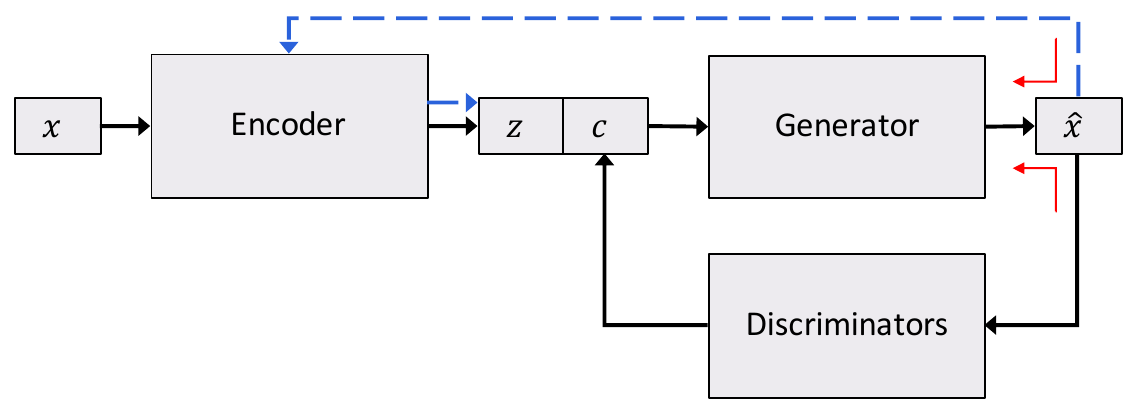
\includegraphics[width=0.5\textwidth]{images/toward1.png}
    \caption
    [نمایی نحوه آموزش مدل \towardctg.]
    {
        نمایی نحوه آموزش مدل \towardctg. خط‌های آبی و سفید جهت حرکت داده و خط‌های قرمز جهت انتفال گرادیان را مشخص می‌کنند \cite{toward}.}
    \label{fig:toward}
\end{figure}
همان‌طور که در شکل \ref{fig:toward} مشخص است، این مدل از ۳ بخش کلی تشکیل شده است؛ یک کدگذار، یک مولد و یک یا چند \discriminator{} که در شکل به جهت سادگی تنها یک نمونه از آن آورده شده است. اگر $c$ نشانگر شرط مورد نظر باشد، وظیفه کدگذار کد کردن جمله ورودی به فضای نهانی است که $c$ در آن ظاهر نشده باشد؛ از سوی دیگر مولد یا در ادبیات مدل‌های پیشین همان کدگشا وظیفه برگرداندن متغیر نهان بدست آمده از کدگذار به جمله اصلی البته با در نظر گرفتن شرط $c$ را داشته و در نهایت \discriminator{} موظف به نظارت بر وجود و رعایت شرط $c$ در جمله تولید شده توسط مولد است. در واقع می‌توان مدل را به صورت یک \vae{} شرطی به همراه یک شبکه \discriminator{} دید که وظیفه نظارت بر شرط مورد نظر را دارد. جهت آموزش این مدل و در نظر گرفتن ویژگی‌های ذکر شده، تابع هزینه از چندین قسمت تشکیل شده است که به اختصار راجع به آن‌ها توضیح داده خواهد شد.
\paragraph*{آموزش کدگذار و مولد}
مطابق با آنچه توضیح داده شد اولین بخش از تابع هزینه مربوط به تابع هزینه شبکه‌های \vae{} شرطی ساده بوده که کنترل‌کننده وظیفه کد کردن و برگرداندن آن به جمله با ویژگی مورد نظر را بر عهده دارد. اگر $E$ کدگذار، $G$ مولد و $D$ \discriminator{} باشد، خواهیم داشت:
\begin{equation}
\begin{split}
L_{VAE} (E, G) =& \expected_{\bff{x} \sim p_{data}} [KL (q_E(\bff{Z}|\bff{x}) || N(\textbf{\latin{0}},\textbf{\latin{I}})) - \expected_{\bff{z} \sim q_E(\bff{Z}|\bff{x}), c \sim q_D(C|\bff{x})} [\log p_G(\bff{x}|\bff{z},c)]].
\end{split}
\end{equation}
از سوی دیگر باید جمله تولیدی توسط مولد حامل ویژگی مورد نظر باشد \cite{toward}. بنابراین تابع هزینه ذیل در نظر گرفته شده است:
\begin{equation}
\begin{split}
L_{att, c} (G) =& -\expected_{\bff{z} \sim p(\bff{Z}), c \sim p(C)} [\log q_D(c|G(\bff{z}, c))]
\end{split}
\end{equation}
که $p(c)$ و $p(\bff{z})$
\trans{توزیع پیشین}{Prior distribution}
تعریف شده روی متغیرهای مربوطه هستند. به عبارت دیگر ابتدا تعدادی نمونه $z$ و $c$ با استفاده از توزیع‌های پیشین تعریف شده ایجاد نموده و سپس مولد بایستی جملاتی را تولید نماید که درست‌نمایی شروط در \discriminator{}‌های مربوطه بیشینه شود.\\
آخرین تابع هزینه‌ای که برای این بخش از مدل در نظر گرفته شده مربوط به حذف وابستگی بین متغیرهای $z$ و $c$ است. به عبارت دیگر مولد بایستی $z$ و $c$ را به جمله‌ای تبدیل نماید که اگر این جمله توسط کدگذار مجددا کد گردد، همان $z$ اولیه بدست آید و جنبه دیگری غیر شروط مورد نظر در جمله تغییر نکرده باشد \cite{toward}. این تابع به شکل زیر تعریف گردیده است:
\begin{equation}
\begin{split}
L_{att, z} (G) =& -\expected_{\bff{z} \sim p(\bff{Z}), c \sim p(C)} [\log q_E(\bff{z}|G(\bff{z}, c))].
\end{split}
\end{equation}
در واقع از سوی دیگر می‌توان کدگذار را به عنوان یک \discriminator{}‌ مشاهده کرد که وظیفه نظارت بر حفظ محتوای جمله غیر از شروط مورد نظر را دارد.
\paragraph*{آموزش دسته‌بند}
بخش دیگر مربوط به آموزش دسته‌بند می‌باشد؛ اینکه دسته‌بند برچسب شرط هر جمله را به درستی پیش‌بینی کند. لازم به ذکر است که برای هر ویژگی یا شرط، یک دسته‌بند مستقل وجود دارد. برای مثال اگر یک ویژگی زمان فعل و دیگری قطبیت آن باشد، دو دسته‌بند، یکی برای زمان فعل و دیگری برای قطبیت آموزش داده خواهد شد \cite{toward}. بخش اول تابع هزینه شبکه دسته‌بند به شکل ذیل است:
\begin{equation}
\begin{split}
L_{s} (D) =& -\expected_{(\bff{x},c) \sim p_{data}} [\log q_D(c|\bff{x})].
\end{split}
\end{equation}
علاوه بر تابع هزینه فوق، حالتی دیگری نیز که بر اساس نمونه‌برداری از فضای نهان شکل می‌گیرد، وجود دارد و به صورت زیر نوشته می‌شود:
\begin{equation}
\begin{split}
L_{u} (D) =& -\expected_{\bff{z} \sim p_\bff{Z}(\bff{Z}), c \sim p(C), \bff{x} \sim p_G(\bff{X}|\bff{z},c)} [\log q_D(c|\bff{x}) + \beta H(q_D(C'|\bff{x}))]
\end{split}
\end{equation}
که $H(q)$ آنتروپی توزیع $q$ و $\beta$ ضریب تنظیم کننده است که بیشنیه میگردد \cite{toward}؛ علت این موضوع نیز آن است که به دلیل امکان وجود خطا در خروجی \decoder{}، \classifier{} نمیبایستی با قطعیت راجع به برچسب آن اظهار نظر کند؛ در واقع این تابع هزینه به نوعی وظیفه \augmentation{} دارد.
در نهایت توابع هزینه به شکل زیر خواهند بود:
\begin{equation}
\begin{split}
L (D) &= L_{s} (D) + \lambda_u L_{u} (D)\\
L (G) &= L_{VAE} (G) + \lambda_c L_{att, c} (G) + \lambda_z L_{att, z} (G)\\
L (E) &= L_{VAE} (E)
\end{split}
\end{equation}
که $(\lambda_s, \lambda_u, \lambda_c , \lambda_z)$ همگی ضرایب تنظیم‌کننده هستند. از دیگر نقاط قوت این مدل باید به دو مورد زیر نیز اشاره نمود:
\renewcommand{\labelitemi}{$\bullet$}
\begin{itemize}
    \item
    
    آموزش
    \trans{نیمه‌نظارتی}{Semi-supervised}:
    همان‌طور که در روابط و نمای کلی مدل مشخص است، تابع هزینه $L_{VAE}$ نیازی به داده برچسب زده شده نداشته و به شکل \semisupervised{} آموزش می‌بیند. در واقع برای آموزش کل مدل به تعداد زیادی جمله بدون برچسب و تعداد کمتری که در حدود ۳۰۰ جمله که در مقاله ادعا شده است برای برچسب‌زنی نیاز است.
    \item
    عدم نیاز به داده 
    \trans{جفت برچسب زده شده}{Jointly labeled}:
    از آنجا که هر شرط مستقل از سایر شروط و برای هر یک، یک دسته‌بند و آموزش مجزا در نظر گرفته شده است، بنابراین نیازی به داده جفت برچسب‌زده شده نیست.
\end{itemize}

\subsection{مدل‌های مبتنی بر \gan{}}
\subsubsection{\cgan{}}
در مورد\gan{} نیز شرایطی مشابه \cvae{} حاکم است و شرط به مولد و \discriminator{}، ورودی داده می‌شود \cite{cgan} و رابطه آن به شرح زیر است:
\begin{align}
	\mcal{V}_\text{CGAN}(D, G) =
	\expected_{(\bff{x}, c) \sim \prob_\text{Data}} [\log D(\bff{x}|c)] +
	\expected_{c \sim p(C), \bff{z} \sim N(\bff{0}, \bff{I}),\bff{x} \sim p_G(\bff{X}|z,c)} [\log 1 - D(\bff{x}|c)]
\end{align}
که نسبت به $D$ بیشینه و نسبت به $G$ کمینه می‌گردد.
\begin{figure}[H]
	\centering
	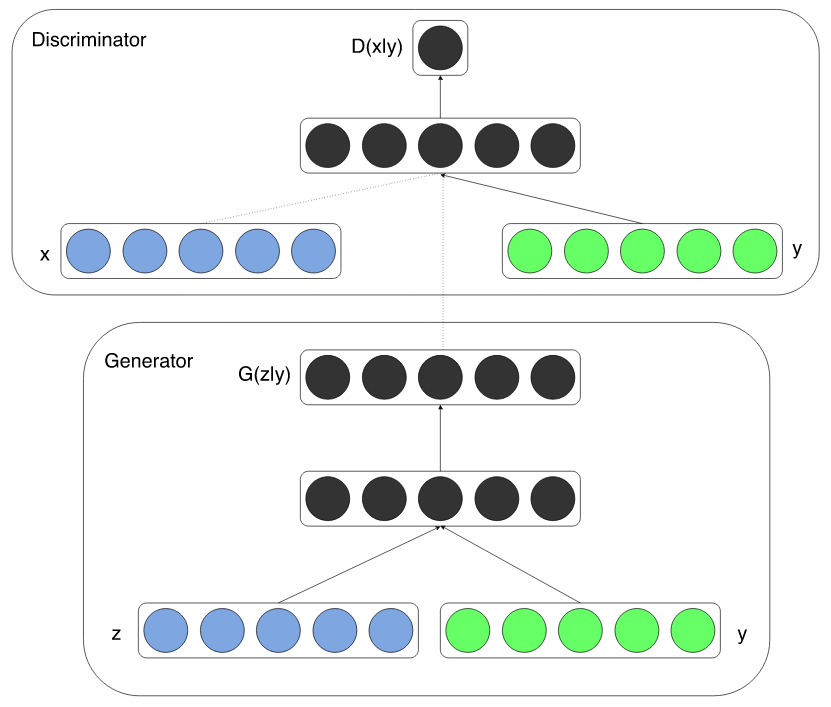
\includegraphics[width=.7\textwidth]{images/cgan.png}
	\caption{نمایی از \cgan{} \cite{cgan}}
    \label{fig:chap2:cgan}
\end{figure}
لازم به ذکر است که مجددا در رابطه فوق مشکل گذر گرادیان وجود دارد و معمولا از روش‌هایی مانند آنچه در بخش \ref{chap2:seqgan} (بر پایه یادگیری تقویتی) است، استفاده می‌شود. نمایی از \cgan{} در شکل \ref{fig:chap2:cgan} آمده است.

\subsubsection{
    تولید جملاتِ با تمایل، با استفاده از شبکه‌های تخاصمی مخلوط
     (\lr{SentiGAN})\protect\LTRfootnote{Generating Sentimental Texts via Mixture Adversarial Networks (SentiGAN)}
}
در این مدل به منظور تولید جمله با $C$ قطبیت معین، به ازای هر مقدار شرط یک مدل مولد مجزا و یک
\trans{دسته‌بند}{Classifier} $C+1$
کلاسه آموزش می‌دهد \cite{sentigan}؛ در این دسته‌بند یک دسته نشانگر داده مصنوعی و سایر دسته‌ها نشان‌گر مقادیر مختلف شرط هستند. در واقع هر مولد سعی در تولید جمله‌ای دارد که از نظر \classifier{} جمله از دسته شرط مرتبط تشخیص داده شده و در مقابل \classifier{} سعی بر نسبت دادن تمام جملات تولید شده توسط مولد‌ها را به دسته $C+1$ام و جملات دادگان اصلی به دسته متناظرشان را دارد و از این جهت همچنان یک \minmaxgame{} در جریان است. اگر
$\{ \bff{x}^n \}_{n=1}^N$
نمونه‌های از توزیع مولد $c$ام با حداکثر طول $T$ باشد، تابع هزینه مدل مولد $c$ام به شرح زیر است:
\begin{align}
	\mcal{L}_\text{SentiGAN}(G_c) = \frac{1}{N}
	\sum_{\bff{x}^n} \sum_{t=1}^{T}
	G_c(\bff{x}^n_t|\bff{x}^n_{1:t-1})
	V_{D_c}(\bff{x}^n_{1:t}, G_c)
\end{align}
که $D_c$ امتیاز \discriminator{} برای دسته $c$ام و تابع $V_{D_c}(., G_c)$ نیز پاداش نسبت داده شده به حرکت $t$ام از مولد $c$ است که برای محاسبه آن مجددا مانند مدل \lr{SeqGAN} (بخش \ref{chap2:seqgan}) از  \montecarlosearch{} برای تخمین پاداش این حرکت استفاده می‌شود. تعریف صوری این پاداش به صورت زیر است:
\begin{align}
	V_{D_c}(\bff{x}_{1:t}, G_c) = \frac{1}{N'} \sum_{n'=1}^{N'} (1 - D_c(\bff{x}_{1:t}, \bff{x}^{n'}_{t+1:T}))
\end{align}
در واقع با ثابت نگه‌داشتن $\bff{x}_{1:t}$،
$N'$
بار جمله را با $G_c$ تکمیل کرده و در نهایت امتیاز \discriminator{} به  $N'$ جمله میانگین گرفته می‌شود. واضح است که برای حرکت آخر (زمانی که $t=T$ است) چنین فرآیندی انجام نمی‌گیرد و از امتیاز \discriminator{} به کل جمله استفاده می‌شود \cite{sentigan}. قابل توجه است که $\mcal{L}_\text{SentiGAN}(G_c)$ با تابع هزینه \wgan{} نیز شبیه بوده، گرچه شرط \lr{K-Lipschitz} بودن برای آن رعایت نشده است
( $G_c(.)V_{D_c}(.)$
به عنوان تابع \critic{} در نظر گرفته شده است).
\\
تابع هزینه دسته‌بند نیز به صورت زیر تعریف می‌شود \cite{sentigan}:
\begin{align}
	\mcal{L}_\text{SentiGAN} (D) =
	- \sum_c \expected_{\bff{x} \sim p_{G_c}} \log D_{C+1} (\bff{x})
	- \expected_{\bff{x} \sim p_\text{Data}(.|c)} \log D_c(\bff{x})
\end{align}

مشخص است که با افزایش تعداد شرط‌ها، این مدل مقیاس‌پذیر نخواهد بود. برای مثلا اگر بخواهیم دو شرط ۳ و ۴ مقداره را مدل کنیم به ۱۲ مدل مولد نیاز است.
\subsubsection{
    مدل مولد برای تولید متن با شرط‌های مقدار گسسته
(\lr{CSGAN})\protect\LTRfootnote{A Generative Model for Category Text Generation (CSGAN)}}
این مدل نیز شباهت زیادی به مدل \cgan{} دارد. نکته اصلی تفاوت آن با \cgan{} در داشتن سیگنال پاداشی متفاوت است. در \cgan{}،
\discriminator{}
ضمن دریافت جفت جمله و شرط، احتمال نسبت به دسته واقعی یا مصنوعی بودن آن را تعیین می‌کرد؛ از این احتمال به عنوان پاداش در ساختار \reinforce{} برای حل گذر گرادیان استفاده شد. در این مقاله علاوه بر \discriminator{} ذکر شده، یک \classifier{} نیز به کار گرفته شده است و از ترکیب امتیاز واقعی بودن و تعلق جمله به دسته شرط مورد نظر، سیگنال پاداشی غنی‌تری ساخته شده است \cite{csgan}. ضمن حفظ ساختار کلی \cgan{}، دسته‌بند $D_C$ با تابع هزینه ذیل آموزش داده می‌شود:
\begin{align}
	\mcal{L}_\text{CGAN} (D_C) =
	-\expected_{(\bff{x}, c) \sim p_\text{Data}} [\log D_C(c|\bff{x})]
	-\expected_{c \sim p_C, \bff{x} \sim \prob_G(.|c)} [\log D_C(c|\bff{x})]
\end{align}
اگر \discriminator{} را با $D_R$ نشان دهیم، تابع پاداش نیز به شکل زیر تغییر می‌کند:
\begin{align}
	\text{Reward} (\bff{x}, c) =
	\frac{2 D_R(\bff{x},c)D_C(c|\bff{x})}
	{D_R(\bff{x},c) + D_C(c|\bff{x})}
\end{align}
در واقع چه طبیعی نبودن جمله و چه عدم تعلق جمله مورد نظر به دسته شرط مورد نظر باعث جریمه مولد خواهد شد و بالعکس.

\section{برخی مفاهیم دیگر}
در این بخش دو مطلب دیگر که یکی رویکرد آموزشی نوین و دیگری معماری نوینی که در حوزه متن اخیرا مورد توجه قرار گرفته است، توضیح داده خواهد شد.
\subsection{\normalizingflownets{}} \label{chap2:flow}
در کنار دو عضو بزرگ از خانواده شبکه‌های مولد مبتنی بر \vae{} و \gan{}، نوع دیگری از شبکه‌ها به نام 
\trans{شبکه‌های مبتنی بر جریان نرمال‌کننده}{Normalizing Flow Networks}
وجود دارند. یکی از مشکلات اساسی ما در این دو نوع \vae{} و \gan{} این است که توانایی محاسبه \likelihood{} به صورت کارا و بدون استفاده از کران‌های پایین و یا بالا وجود ندارد. برای مثال در \vae{} کران پایین \likelihood{} را بیشینه کرده \cite{vae} و در \gan{}‌ها نیز از تابع هزینه دیگری استفاده می‌شود و در مورد رابطه آن با \likelihood{} صحبت شفافی نمی‌توان کرد \cite{gan} (عدم امکان محاسبه \likelihood{} در \gan{} به صورت کلی بیان شد؛ این در حالی است که در حوزه متن امکان محاسبه آن وجود دارد).  بر خلاف این دو دسته، خانواده \normalizingflownets{} توانایی نمونه‌گیری و محاسبه \likelihood{} به صورت کارا را داشته و یا حداقل سعی بر این موضوع دارند \cite{flow_survey}. بنابراین امکان بهینه‌سازی مدل نسبت به تابع هزینه‌ای بر مبنای مقدار دقیق \likelihood{} امکان پذیر است. از سوی دیگر همان طور که تا به اینجا توضیح داده شد، سختی‌ها و نقاط ضعفی از قبیل تنوع نداشتن نمونه‌ها در \gan{} و یا صفر شدن بخش \lr{KL} در \vae{} وجود دارد. این در حالیست که در \normalizingflownets{} با بهینه‌سازی بر اساس \likelihood{} مشکل کم بودن تنوع نمونه‌ها وجود نداشته و یا مشکلات آموزش مانند آنچه ذکر شد، گزارش نشده است. البته این نکته قابل ذکر است که در صورت کم بودن ظرفیت مدل نسبت به توزیع هدف مورد نظر، تابع هزینه مبتنی بر \likelihood{} رفتار \meanseeking{} از خود بروز داده و توزیعی را یاد خواهد گرفت که تمام نقاط را پوشش دهد. بدیهیست که ممکن است برای پوشش دادن تمام نقاط نقاطی نامطلوب را نیز پوشش دهد.
\subsubsection{مفاهیم پایه}
فرض کنید
${\bf{ Z}} \in \mathbb{R}^{D}$
متغیر تصادفی با تابع چگالی احتمال مشخص
$p_{\bf Z}: \mathbb{R}^D$
و $\bf f$ تابعی معکوس پذیر و
${\bf Y} = {\bf f}({\bf Z})$
است. حال با استفاده از قانون تغییر متغیر می‌توان رابطه زیر را نوشت:
\begin{align}  \label{eq:flow_target_dist}
p_{\bf Y}({\bf y}) = & p_{\bf Z}({\bf g}({\bf y}))
|\text{det} ~ \text{D} {\bf g}({\bf y})|
\nonumber                                          \\
=                    & p_{\bf Z}({\bf g}({\bf y}))
|\text{det} ~ \text{D} {\bf f}({\bf g}({\bf y}))|^{-1}
\end{align}
که $\bf g$ تابع معکوس $\bf f$ و
$\text{D} {\bf g}({\bf y}) = \frac{\partial {\bf g}}{\partial {\bf y}}$
ماتریس ژاکوبین تابع $\bf g$ و
$\text{D} {\bf f}({\bf z}) = \frac{\partial {\bf f}}{\partial {\bf z}}$
ماتریس ژاکوبین تابع $\bf f$ است. تابع چگالی احتمال حاصل از اعمال تابع $\bf f$ به توزیع پایه را با
$f_*p_{\bf Z}$
نشان خواهیم داد.

در ادبیات مدل‌های مولد، تابع $\bf f$ به عنوان مولد، توزیع پایه
$p_{\bf z}$
را به توزیعی پیچیده‌تر تبدیل می‌کند که به حرکت از توزیع پایه به توزیع نهایی را جهت مولد می‌نامند. به منظور نمونه‌برداری از توزیع نهایی نیز می‌توان از توزیع پایه نمونه برداری کرده و با استفاده از تابع
${\bf y} = {\bf f} ( {\bf z} )$
به نمونه از توزیع نهایی رسید. در جهت مخالف، برای تبدیل توزیع نهایی به توزیع پایه که معمولا توزیع گاوسی نرمال انتخاب می‌شود، از تابع $\bf g$ بهره برده می‌شود. به همین دلیل انتخاب نام جریان نرمال‌کننده بدون هدف نبوده و در واقع جهت مخالف مربوط به تبدیل توزیع پیچیده نهایی به توزیع پایه گاوسی نرمال است \cite{flow_survey}.
\\
به طور کلی اگر تابع $\bf f$ یک تبدیل پیچیده باشد، توانایی تولید هر توزیعی وجود خواهد داشت؛ به عبارت دیگر به ازای هر توزیع هدف
$ p_{\bf Y}({\bf y})$
تابع $\bf f$ای وجود خواهد داشت که
$ p_{\bf Y}({\bf y}) = f_*p_{\bf Z}$.
اما به منظور آموزش و نمونه‌گیری کارا، نیاز است تا این توابع ویژگی‌های خاصی به شرح ذیل داشته باشند \cite{flow_survey}:
\begin{itemize}
    \item
    معکوس‌پذیر باشند. ممکن است تابع معکوس در جهت نمونه‌گیری و یا جهت نرمال‌ساز به کار برده شود.
    \item
    به اندازه کافی پیچیده باشند تا بتواند توزیع داده اصلی را مدل کنند.
    \item
    به لحاظ محاسباتی کارا باشند. برای محاسبه \likelihood{} یک نمونه و نمونه‌گیری نیاز است تا هر دو جهت نمونه‌گیری و نرمال‌ساز به صورت کارا محاسبه شوند. علاوه بر این، طبق رابطه \ref{eq:flow_target_dist} برای محاسبه  \likelihood{} یک نمونه در توزیع نهایی، به محاسبه کارای دترمینان ماتریس ژاکوبین تابع $\bf f$ نیاز است. بنابراین بایستی دترمینان ماتریس ژاکوبین تابع $\bf f$ نیز به صورت کارا محاسبه شود.
\end{itemize}
این خانواده از مدل‌های مولد شامل چندین دسته هستند که در ادامه معرفی خواهند شد.
\subsubsection{جریان‌های
    \trans{درایه‌گرا}{Elementwise}}
یک فرم پایه از توابع غیرخطی معکوس‌پذیر را می‌توان از توابع \elementwise{} ساخت. فرض کنید تابع
$h: \mathbb{R} \rightarrow \mathbb{R}$
باشد و معکوس‌پذیر است. اگر
${\bf x} = (x_1, x_2, ..., x_D)^T$
خواهیم داشت:
\begin{gather}
{\bf f}({\bf x}) = (h(x_1), h(x_2), ..., h(x_D))^T
\end{gather}
برای محاسبه تابع معکوس به تابع $h^{-1}$ نیاز است و از آنجا که ماتریس ژاکوبین آن قطری است پس دترمینان آن ضرب المان‌های روی قطر آن خواهد شد. در واقع چنین تابعی مانند توابع فعال‌سازی مورد استفاده در شبکه‌های عصبی هستند؛ با این تفاوت که این توابع معکوس پذیر نیستند. برای مثال تابع \lr{ReLU} معکوس پذیر نیست اما \lr{ELU} است. به دلیل اینکه این توابع به صورت \elementwise{} عمل می‌کنند، پیچیدگی لازم را ندارند. مدل‌های بعدی سعی در پوشش این ضعف دارند \cite{flow_survey, realnvp, iaf, maf}.
\subsubsection{جریان‌های خطی}
یک تبدیل خطی به طور کلی به شکل زیر تعریف می‌شود:
\begin{align}
{\bf f}({\bf x}) = {\bf A}{\bf x} + {\bf b}
\end{align}
که $A \in \mathbb{R}^{D \times D}$ و $b \in \mathbb{R}^D$ پارامتر‌های این تبدیل هستند. دترمینان این تبدیل برابر با دترمینان ماتریس ${\bf A}$ بوده و برای معکوس آن نیاز به ${\bf A}^{-1}$ است.
این دو عملیات در حالت کلی با مرتبه زمانی
$O(D^3)$
قابل انجام هستند. اگر توزیع پایه از نوع توزیع‌های نمایی باشد، بعد از اعمال تبدیل فوق در خانواده توزیع‌های نمایی باقی می‌ماند. با این وجود، این دسته یکی از پایه‌های اصلی توابع پیچیده هستند. برای تقلیل زمان محاسبه دترمینان و معکوس تابع، به عناوین مختلف سعی در محدود کردن شکل آن‌ها شده تا این اعمال به صورت کارا انجام پذیرند. برای مثال از پارمتری کردن ${\bf A}$ به صورت پایین مثلثی یا بالا مثلثی بهره برده می‌شود تا دترمینان به صورت بسیار ساده و با ضرب المان‌های روی قطر بدست آید و ماتریس معکوس نیز در $O(D^2)$ محاسبه شود. از آنجا که قدرت این تبدیل وابسته به ترتیب اعمال شده به ابعاد است (هر بعد تابعی از بُعدهای قبل از خود است)، راهکارهای متفاوتی از قبیل تغییر ترتیب به صورت تصادفی و یا یافتن یک ماتریس تبدیل متعامد (حالت کلی‌تر تغییر ترتیب در بعدها) ارائه شده است \cite{flow_survey, glow}.
\subsubsection{جریان‌های
    \trans{اتصالی}{Coupling}
}
در این گونه از تبدیل‌ها، فضای ورودی به دو زیرفضا تقسیم می‌شود. اگر فضای ورودی را با
$\bff{x} \in \bb{R}^D$
نشان دهیم، دو زیرفضا از آن به صورت
$(\bff{x}^A, \bff{x}^B) \in \bb{R}^d \times \bb{R}^{D - d}$
، تابع معکوس‌پذیر
$\hat{\bff{f}}(.; \theta) : \bb{R}^D \rightarrow \bb{R}^D$
را در نظر بگیرید. یک جریان \coupling{}
$f : \bb{R}^D \rightarrow \bb{R}^D$
را به شکل زیر می‌توان تعریف نمود:
\begin{align}
\bff{y}^A = & \hat{\bff{f}} (\bff{x}^A; \Theta(\bff{x}^B))
\nonumber
\\
\bff{y}^B = & \bff{x}^B
\end{align}
که $\Theta(\bff{x}^B)$ یک تابع کاملا پیچیده از $\bff{x}^B$ است که به آن
\trans{شرطی‌کننده}{Conditioner}
، به تابع $\hat{\bff{f}}$ یک لایه \coupling{} و به کل تابع $\bff{f}$ یک جریان \coupling{} گفته می‌شود. نمایی از این جریان در شکل \ref{fig:chap2:flow_coupling} آمده است. معکوس‌پذیری این جریان در گرو معکوس‌پذیری لایه \coupling{} است و در این صورت به شکل زیر محاسبه می‌گردد:
\begin{align}
\bff{x}^A = & \hat{\bff{f}}^{-1} (\bff{y}^A; \Theta(\bff{y}^B))
\nonumber
\\
\bff{x}^B = & \bff{y}^B
\end{align}
ماتریس ژاکوبین این تابع نیز به صورت یک
\trans{ماتریس مثلثی بلوکی}{Block triangular matrix}
است که یکی از بلوک‌های آن ماتریس همانی و دیگری $\text{D}\hat{\bff{f}}$ است. بنابراین دترمینان  تابع $\bff{f}$ دترمینان برابر تابع $\hat{\bff{f}}$ است \cite{flow_survey, realnvp, glow}.

\begin{figure}[H]
    \centering
    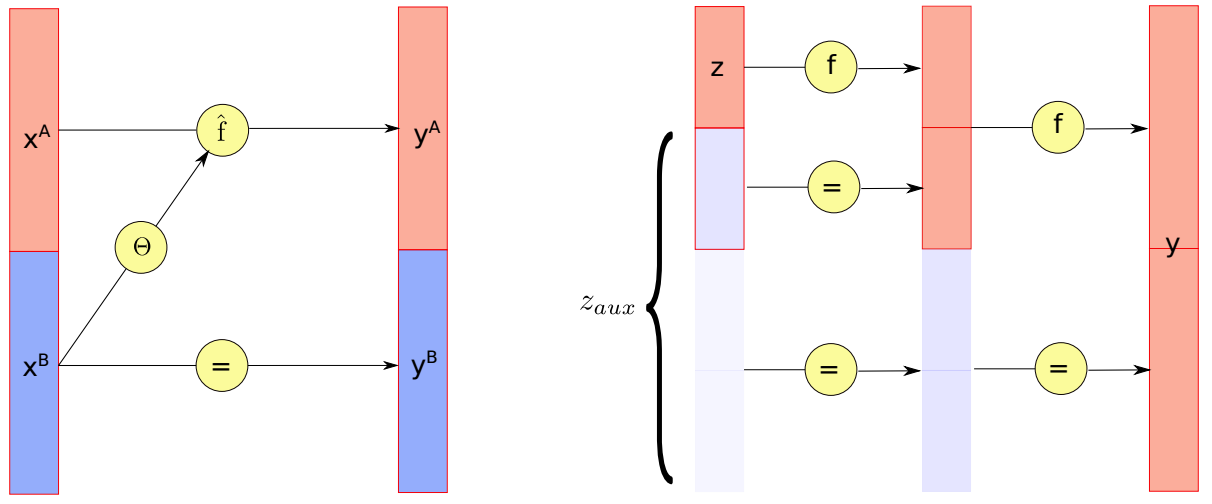
\includegraphics[width=.7\textwidth]{images/flow-survey1.png}
    \caption{
        نمایی از جریان‌های \coupling{}
        \cite{flow_survey}	}
    \label{fig:chap2:flow_coupling}
\end{figure}

در واقع قدرت اصلی این تابع در میزان پیچیده بودن تابع $\Theta$ است و می‌توان آن را با شبکه عصبی مدل نمود. لازم به ذکر است که این تابع می‌تواند تابعی از $\bff{x}^B$ نباشد و به عنوان اضافه کردن بُعد به کار بسته شود. اما مشکل این تبدیل در نحوه شکستن فضای ورودی به دو فضا است. روش‌های مختلفی نیز از جمله تغییر ترتیب ابعاد به صورت تصادفی برای حل این مشکل ارائه شده است.
\subsubsection{جریان‌های \autoregressive{}}
می‌توان مدل‌های \autoregressive{} را مدل‌هایی از جنس \normalizingflownets{} و نسخه غیر خطی ضرب ماتریس مثلثی در نظر گرفت \cite{flow_survey, iaf, maf}.
\\
مجددا اگر فضای ورودی با
$(x_1, x_2, ..., x_D) = \bff{x} \in \bb{R}^D$
نشان داده شود و
$\hat{\bff{f}} : \bb{R} \rightarrow \bb{R}$
یک تابع معکوس‌پذیر باشد، با داشتن یک ترتیب ثابت بر روی فضای ورودی، تابع \autoregressive{}
$\bff{y} = \bff{f} : \bb{R}^D \rightarrow \bb{R}^D$
به صورت زیر تعریف می‌شود:
\begin{align}
y_t = \hat{\bff{f}}(x_t; \Theta_t(x_{1:t-1}))
\end{align}
که $t= 2, 3, ..., D$
، $\Theta_t$
یک تابع پیچیده از $\bb{R}^{t-1}$ به فضای پارامترهای تابع $\bff{f}$ و $\Theta_1$ یک تابع ثابت است. در اینجا نیز به $\Theta_t$ یک \conditioner{} گفته می‌شود.
\\
از آنجا که $y_t$ تنها تابعی از $x_{1:t-1}$ است، ماتریس ژاکوبین این تابع نیز مثلثی بوده و بنابراین دترمینان آن از ضرب عناصر قطر آن بدست می‌آید. با داشتن تابع معکوس $\hat{\bff{f}}$، معکوس تابع $\bff{f}$ قابل محاسبه است؛ اما از آنجا که ساختار \autoregressive{} بر روی ابعاد حاکم است، بنابراین  باید هر بعد به صورت ترتیبی از ابعاد قبل به دست آید و درنتیجه نمی‌توان از پتانسیل موازی‌سازی \gpu{} بهره برد. به منظور موازی‌سازی در جهت نمونه‌گیری، می‌توان از ساختار شبکه‌های \lr{MADE} بهره برد. این شبکه به این صورت است که هر بُعد از آن تنها تابعی از ابعاد قبل از خود است. نمایی از این شبکه در شکل \ref{fig:chap2:made} آمده است \cite{made}.
\begin{figure}[h]
    \centering
    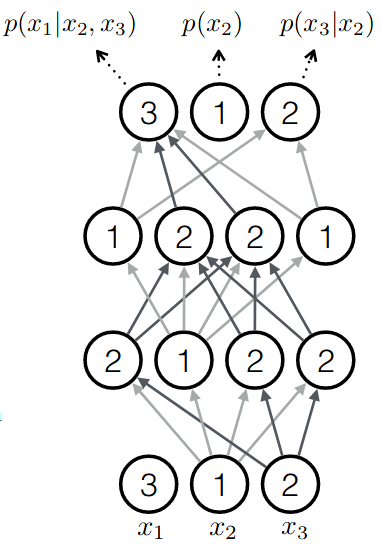
\includegraphics[width=.25\textwidth]{images/made.png}
    \caption{
        نمایی از مدل \lr{MADE}
        \cite{made}.
    }
    \label{fig:chap2:made}
\end{figure}
در صورت استفاده از ساختار شبکه \autoencoder{} نقابی برای تخمین توزیع (\lr{MADE})
\LTRfootnote{Masked Autoencoder for Distribution Estimation (MADE)}
در $\Theta$، به آن 
جریان \autoregressive{} نقابی (\lr{MAF})
\LTRfootnote{Masked Autoregressive Flow (MAF)}
گفته می‌شود \cite{maf}.

\begin{figure}[h]
    \centering
    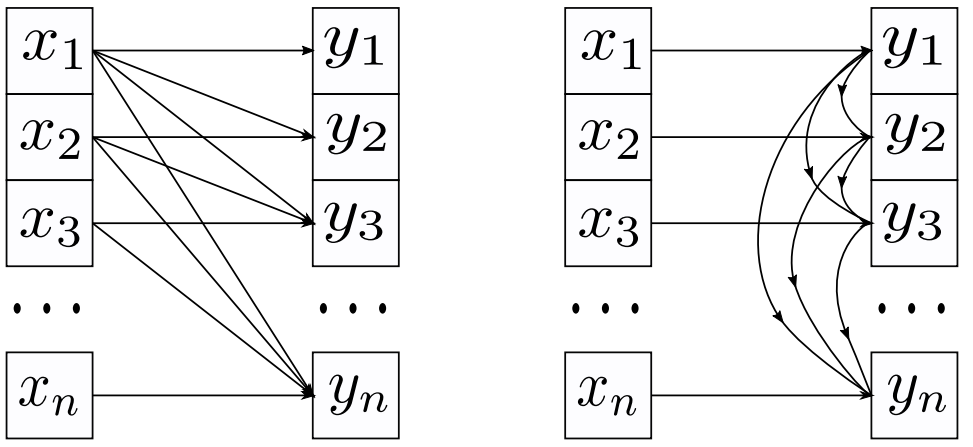
\includegraphics[width=.5\textwidth]{images/flow-survey2.png}
    \caption{
        تفاوت مدل‌های \lr{MAF} و \lr{IAF} به زبان تصویر \cite{iaf, maf, flow_survey}
    }
    \label{fig:chap2:mafvsiaf}
\end{figure}

مدل‌سازی تابع \autoregressive{}
$\bff{f}$
را می‌توان به صورت زیر نیز تعریف کرد:
\begin{align}
y_t = \hat{\bff{f}}(x_t; \Theta_t(y_{1:t-1}))
\end{align}
که در واقع عکس روش \lr{MAF} است. به همین دلیل این روش را جریان \autoregressive{} معکوس (\lr{IAF})
\LTRfootnote{Inverse Autoregressive Flow (IAF)}
می‌نامند \cite{iaf, flow_survey}. در واقع در \lr{MAF} رفتن از توزیع پایه به توزیع نهایی کُند و رفتن از توزیع نهایی به توزیع پایه سریع است؛ در حالی که \lr{IAF} نمونه‌برداری سریع اما جریان نرمال‌کننده کندی دارد و بایستی بسته به نیاز از آن‌ها بهره برد. تفاوت این مدل در شکل \ref{fig:chap2:mafvsiaf} مشخص است.
نکته قابل ذکر در مورد دسته \autoregressive{}  از \normalizingflownets{} این است که در  بعضی موارد اثبات شده است که این خانواده از توابع، توانایی مدل کردن هر تابعی را داشته و به اصطلاح یک
\trans{تخمین‌‌گر عمومی}{Universal approximator}
هستند \cite{flow_survey}.
\subsubsection{لایه‌های \coupling{}}
تا به اینجا در مورد خانواده‌های مختلف \normalizingflownets{} صحبت شد. در تمام آن‌ها از توابع معکوس‌پذیر استفاده شده اما در مورد ساختار آن‌ها توضیحی داده نشد. در این بخش به توضیح تعدادی از توابع معکوس پذیر مورد استفاده پرداخته خواهد شد.
\paragraph*{لایه
    \coupling{} \trans{هم‌نسبی}{Affine}}
این لایه‌های خطی، ساده‌ترین و رایج‌ترین لایه‌های مورد استفاده در \normalizingflownets{} هستند. اگر لایه مورد نظر با $\hat{\bff{f}}: \bb{R} \rightarrow \bb{R}$ نشان داده شود، به صورت زیر تعریف می‌شود:
\begin{align}
\hat{\bff{f}} (x; \theta) = \theta_1 x + \theta_2, \theta_1 \neq 0, \theta_2 \in \bb{R}
\end{align}
این لایه در مدل‌های بسیاری از جمله \cite{iaf, maf} استفاده شده است.
\paragraph*{لایه \coupling{}
    غیر خطی درجه دو}
نوع پیشرفته‌تر لایه ذکر شده، نسخه غیرخطی آن‌ها می‌باشد. به این صورت که تابع $\hat{\bff{f}}$ برای مثال به صورت یک تابع درجه ۲ در نظر گرفته می‌شود. به طور واضح چنین تابعی بایستی معکوس‌پذیر باشد؛‌ به همین دلیل از شروط مختلفی برای برآوردن آن استفاده می‌گردد. برای مثال این تابع می‌تواند به صورت زیر تعریف شود:
\begin{align}
\hat{\bff{f}}(x; \theta) = ax + b + \frac{c}{1 + (dx + h)^2}
\end{align}
تحت شرایطی پارامترهای $\theta=[a,b,c,d]$ یک تابع معکوس پذیر خواهند ساخت و به این هدف، نیاز به محاسبه ریشه تابع فوق که یک تابع درجه ۳ است، خواهد بود \cite{flow_survey}.
\paragraph*{لایه \coupling{} \spline{}}
این نام که شاید بیش‌تر در محاسبات عددی شنیده شود، به معنی یک تابع
\trans{تکه‌ای چند جمله‌ای}{Piece-wise polynomial}
است. در واقع اگر $K+1$ نقطه وجود داشته باشد، فواصل بین هر دو نقطه با یک تابع چندجمله‌ای مدل خواهد شد (در واقع $K$ تابع وجود خواهد داشت). حال این توابع باید از نقاط تعیین شده عبور کنند و همچنین در مجموع معکوس‌پذیر باشند. برای محاسبه تابع معکوس نیز پس از تعیین اینکه نقطه مورد نظر مربوط به کدامین تابع از $K$ تابع است، ریشه‌ی معادله مربوطه، جواب خواهد بود \cite{flow_survey}.
\paragraph*{لایه \coupling{} عصبی}
نوع کلی‌تری از این لایه‌ها نیز موجود است که با یک شبکه عصبی مدل می‌شوند. به مانند قبل،‌ باید این تابع معکوس‌پذیر باشد؛ برای مثال اگر وزن‌های این تابع همگی مثبت و توابع فعال‌سازی آن یکنوا باشند، این شبکه یک تابع معکوس‌پذیر خواهد بود. در رابطه با این مورد ادعای \univapprox{} نیز وجود دارد \cite{flow_survey}.
\\\\
علاوه بر دسته‌های ذکر شده، دسته‌های دیگری نیز وجود دارند که از حوصله این بحث خارج است. لازم به ذکر است که خانواده \normalizingflownets{} اخیرا بیشتر مورد توجه قرار گرفته و می‌تواند حوزه تحقیقی مورد توجهی باشد.
\subsection{معماری \transformer{}}
معماری‌های معمول استفاده شده در حوزه پردازش متن بیشتر شامل \lstm{} و \cnn{} هستند. اخیرا معماری دیگری به نام \transformer{} مورد توجه قرار گرفت که مخصوص پردازش داده‌های به صورت دنباله بوده و پایه بسیاری از مدل‌های \stateoftheart{} است. در ادامه به معرفی این معماری و اجزای آن پرداخته خواهد شد.
\\
این مدل معماری نیز در گروه مدل‌های
\trans{دنباله به دنباله}{Sequence to sequence}
جای گرفته و از \encoder{} و \decoder{} تشکیل شده است. اگر یک جمله با طول $n$ را با $\bff{x} = (x_1, ..., x_n)$  نشان داده شود، \encoder{} با گرفتن دنباله کلمات $\bff{x}$ (یا هر واحد مورد استفاده دیگر)، این دنباله  را به دنباله بردار‌های پیوسته $\bff{z} = (z_1, ..., z_n)$ تبدیل می‌کند. \decoder{} نیز با گرفتن $\bff{z}$ دنباله کلمات مقصد $\bff{y} = (y_1, ..., y_m)$ خروجی می‌دهد. با اینکه معماری \encoder{} به صورت \autoregressive{} نیست اما \decoder{}، واحدی برای کنترل و ایجاد حالت \autoregressive{} را در خود جای داده است \cite{transformer}.
\begin{figure}[H]
    \centering
    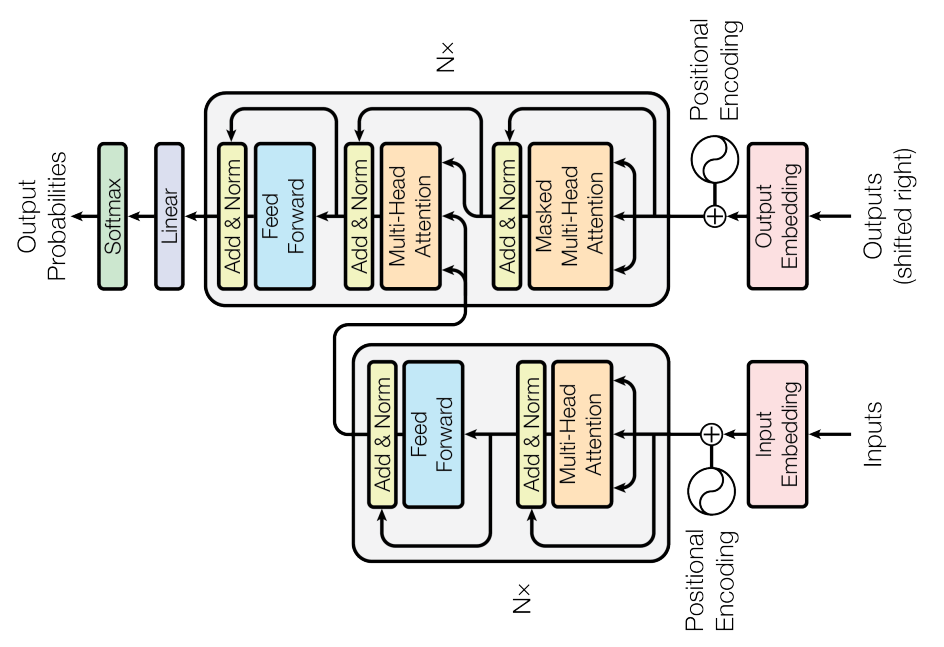
\includegraphics[width=.7\textwidth, angle=-90]{images/attention3.png}
    \caption{
        نمایی از معماری کلی \transformer{} \cite{transformer}}
\end{figure}

\paragraph*{\encoder{}}
\encoder{}
از پشته‌ای $N$ لایه یکسان تشکیل شده است. هر لایه شامل دو زیر لایه است. اولین زیر لایه مربوط به نوعی مکانیزم توجه به نام
\trans{خودتوجه چند سر}{Multi-head Self-attention}
و زیر لایه دوم یک لایه
\trans{تمام متصل}{Fully connected}
است. لازم به ذکر است که در هر زیرلایه از اتصالات
\trans{باقی‌مانده}{Residual}
و
\trans{نرمال‌کننده لایه}{Layer normalization}
استفاده شده است\cite{transformer}.
\paragraph*{\decoder{}}
\decoder{}
نیز از پشته کردن $N$ لایه تشکیل شده است. هر لایه علاوه بر واحد‌های ذکر شده برای \encoder{}، زیرلایه سومی نیز دارد که شامل
\trans{توجه چند سر}{Multi-head Attention}
به خروجی \encoder{} است. در \decoder{} نیز از اتصالات \residual{} و \layernormalization{} استفاده شده است. واحد \multiheadselfattention{} تفاوت کوچکی با واحد مشابه \encoder{} دارد تا در پیشبینی هر کلمه در خروجی، تنها تابعی از کلمات قبل از خود بوده و \autoregressive{} باشد \cite{transformer}.
\\
یک مکانیزم توجه را می‌توان نگاشتی از بردار
\trans{پرسمان}{Query}
و یک مجموعه \keyvaluepair{} به یک بردار در نظر گرفت که \query{}، کلیدها و مقدارها همگی بردارند. بردار خروجی از جمع وزن‌دار بردارهای مقدار و هر وزن نسبت داده شده به بردار مقدار، با تابعی از بردار \query{} و کلید بدست می‌آید. در ادامه به شرح دقیق‌تر این مکانیزم پرداخته خواهد شد.
\subsubsection{مکانیزم
    \trans{توجه با استفاده از ضرب داخلی مقیاس شده}{Scaled Dot-Product Attention}}
این مکانیزم توجه که نام \dotattention{} بر آن نهاده شده است بر روی بردارهای \query{} و کلید $d_k$ بعدی و بردارهای مقدار $d_v$ بعدی اعمال می‌شود. امتیاز هر بردار مقدار با استفاده از ضرب داخلی بردار \query{} در بردار کلید متناظر آن بدست آمده و در نهایت با اعمال تابع \softmax{} بر روی آن وزن مربوطه محاسبه می‌گردد. لازم به ذکر است که برای کنترل واریانس امتیاز هر بردار مقدار، امتیازات قبل از اعمال تابع \softmax{} تقسیم بر $\sqrt{d_k}$ می‌شوند \cite{transformer}.
\begin{figure}[H]
    \centering
    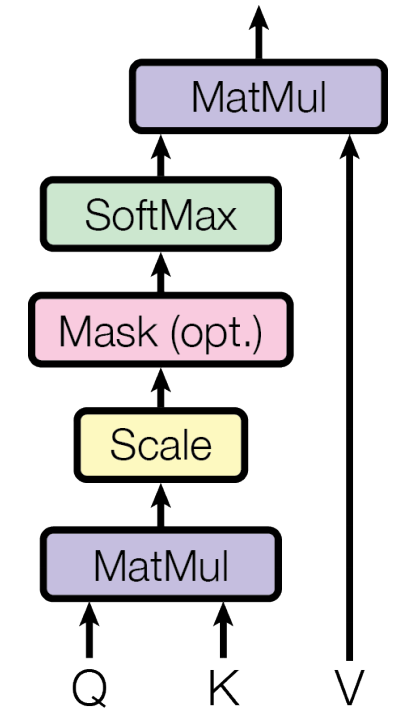
\includegraphics[width=.25
    \textwidth]{images/attention1.png}
    \caption{نمایی از \dotattention{}
        \cite{transformer}.}
\end{figure}
این مکانیزم به صورت زیر می‌توان تعریف کرد:
\begin{align}
\text{Attention}(Q, K, V) = \text{softmax}(\frac{QK^T}{\sqrt{d_k}})V
\end{align}
که
$Q \in \bb{R}^{n \times d_k}$،
$K \in \bb{R}^{n \times d_k}$ و
$V \in \bb{R}^{n \times d_v}$
به ترتیب بردارهای \query{}، کلید و مقدار هستند.
ویژگی \autoregressive{} در همین نقطه به مدل تزریق می‌شود. اگر امتیاز یک بردار مقدار $-\infty$ شود، وزن نسبت داده شده به این بردار پس از اعمال \softmax{} برابر با صفر خواهد بود؛ بنابراین می‌توان به طور دلخواه تاثیر هر بردار مقدار را با نسبت دادن  امتیاز $-\infty$ به آن، صفر کرد. به ماتریس $n \times n$ بُعدی که ردیف $i$ام آن بیان کننده مکان‌های قابل توجه برای کلمه $i$ام است، ماتریس
\trans{نقاب}{Mask}
گفته می‌شود (یک برای مکان‌های قابل توجه و $-\infty$ برای مکان‌های غیرقابل توجه) \cite{transformer}.

\subsubsection{مکانیزم \multiheadattention{}}
این امکان وجود دارد که به جای یک بار اعمال تابع توجه بر بردارهای $d_\text{model}$ بُعدی ($d_\text{model}$ اندازه بردار ورودی است)، بردارهای \query{}، کلید و مقدار را با $h$ تبدیل خطی به ترتیب به $h$ فضای مختلف با ابعاد $d_k$، $d_k$ و $d_v$ بُعدی برده و پس از اعمال تابع توجه، نتایجشان را به یکدیگر متصل کرد. لازم به ذکر است که این عملیات‌ها همگی به موازات یکدیگر  قابل انجامند و می‌توان از پتانسیل موازی‌سازی \gpu{} بهره گرفت. در واقع \multiheadattention{} این امکان را به مدل می‌دهد تا با بردن بردارها به فضاهای متفاوت، از چندین فضای مختلف به مکان‌ها و ویژگی‌های مختلف نگاه کرده و در نتیجه به مکان‌های متفاوتی به صورت همزمان توجه کند \cite{transformer}.
\begin{gather}
\text{MultiHead}(Q, K, V) = \text{Concat}(\text{head}_1, ..., \text{head}_h)W^O \nonumber
\\
: \text{head}_i = \text{Attention}(QW_i^Q, KW_i^K, VW_i^V)
\end{gather}
که
$W_i^Q \in \bb{R}^{d_\text{model} \times d_k},
W_i^K \in \bb{R}^{d_\text{model} \times d_k},
W_i^V \in \bb{R}^{d_\text{model} \times d_v},
W^O \in \bb{R}^{hd_v \times d_\text{model}}$
ماتریس‌های تبدیل خطی هستند. لازم به ذکر است که $h \times d_v = d_\text{model}$ است.
\begin{figure}[H]
    \centering
    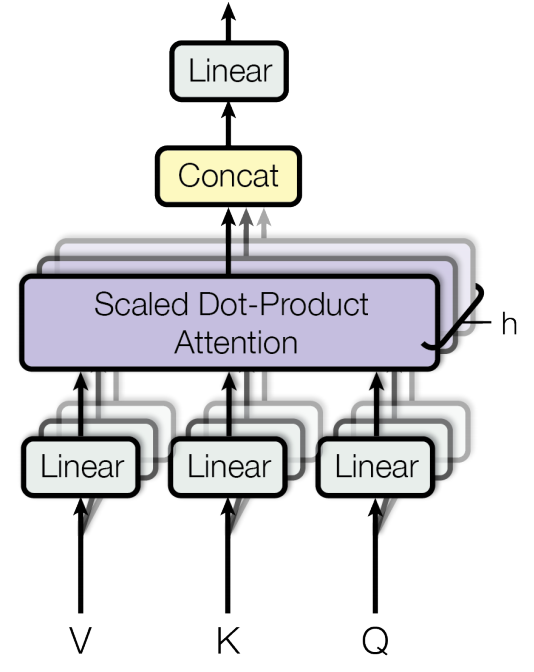
\includegraphics[width=.4
    \textwidth]{images/attention2.png}
    \caption{نمایی از \multiheadattention{}}
\end{figure}
تا به اینجا مکانیزم توجه در \transformer{} توضیح داده شد اما این مکانیزم به چه صورتی و در کجا استفاده شده است؟
\begin{itemize}
    \item
    در \decoder{} واحد \multiheadattention{} وجود دارد. در اینجا \query{} ها، خروجی لایه قبل \decoder{} و بردارهای مقدار و کلید خروجی‌های \encoder{} هستند. در واقع می‌توان از این مکانیزم تعبیر حافظه نیز داشت \cite{transformer}.
    \item
    در \encoder{} نیز از \multiheadselfattention{} نام برده شد. \multiheadselfattention{} همان \multiheadattention{} است اگر که بردار \query{}، کلید و مقدار آن یک چیز باشند. بنابراین به ازای هر کلمه، در هر لایه \encoder{}، به تمام خروجی‌های لایه قبل \multiheadselfattention{} زده می‌شود \cite{transformer}.
    \item
    مجددا در \decoder{} نیز از \multiheadselfattention{} استفاده شده است؛ با این تفاوت که در هر لایه، بردار متناظر با کلمه $i$ با استفاده از \mask{}‌های $-\infty$، تنها تابعی از بردار کلمات قبل‌تر از $i$ خواهد بود \cite{transformer}.
\end{itemize}

\subsubsection{بردار
    \trans{تعبیه مکانی}{Positional Embedding}}
از آنجا که ساختار معرفی شده، خاصیت \recurrence{} ندارد، در هیچ جایی اطلاعاتی راجع به فاصله کلمات نسبت به هم و موقعیتشان در جمله وارد مدل نمی‌شود؛ بنابراین نیاز است تا به نحوی موقعیت کلمات در بردار \embedding{} هر کلمه گنجانده شود که به آن \positionalembedding{} گفته می‌شود. بردار \positionalembedding{}
$PE$
که $d_\text{model}$ بُعدی است، به صورت زیر تعریف شده است \cite{transformer}:
\begin{align}
PE_{(pos, 2i)} = \sin ( pos / 10000^{2i/d_\text{model}}) \nonumber
\\
PE_{(pos, 2i+1)} = \cos ( pos / 10000^{2i/d_\text{model}})
\end{align}
که $pos$ شناسه مکانی مورد نظر است. در مورد نحوه انتخاب روش \encoding{} نیز این طور بیان شده است که
\positionalembedding{}  $i+k$
تابعی خطی از
\positionalembedding{} $i$
است بوده و قابلیت توسعه‌پذیری به جملات با طول‌های بیشتر که در حین آموزش دیده نشده است را ایجاد می‌کند \cite{transformer}. لازم به ذکر است که بردار \positionalembedding{} با بردار \embedding{} کلمه متناظرش جمع خواهد شد.
\newline
در این فصل سعی شد تا در ابتدا فاصله‌های معروف مورد استفاده و سپس مدل‌های زبانی غیر شرطی، به دلیل پایه‌ای بودن این \task{} نسبت به \task{} تولید شرطی، در دو دسته با فضای نهان و بدون فضای نهان، معرفی شوند. در این بین، مشکل عدم توجه به فضای نهان مطرح و راه‌حل‌هایی برای آن ارائه شد. در انتها نیز ضمن شرح معماری نوین \transformer{} و همچنین رویکردِ کمتر مورد توجه \normalizingflownets{}، رویکرد‌های متفاوت آموزش مدل‌های زبانی شرطی توضیح داده شده و مورد بررسی قرار گرفتند.
در فصل بعد ضمن مروری بر ضعف و قوت مدل‌های معرفی شده، مدل پیشنهادی جهت رفع مشکلات ذکر شده و همچنین توانایی در تولید متن به صورت شرطی ارائه خواهد شد.

\chapter{مبانی نظری}\label{chap3}
\minitoc

\section{مقدمه}

پس از تعریف مساله و مرور و بررسی روش‌های پیشنهاد شده توسط پژوهشگران، نوبت به ارائه راهکار پیشنهادی می‌رسد. البته راهکار پیشنهادی در این پژوهش خود بنا شده بر مدل‌های نوین ارائه شده در پردازش زبان است که نیازمند توضیح و بررسی می‌باشند.
از این رو، در این فصل مبانی نظری‌ای که پایه‌ها و ستون‌های راهکار پیشنهادی ارائه شده هستند، بیان و تشریح می‌شوند. در اولین بخش از این فصل معماری ترنسفورمر ارائه خواهد شد. در بخش دوم، شبکه‌های از پیش آموزش داده شده ترنسفورمری نظیر برت و بارت ارائه خواهند شد. آخرین بخش نیز به بررسی بعضی معیارهای سنجش تولید متن پرداخته شده است و یک معیار متفاوت از معیارهای مورد استفاده سایر پژوهش‌های مساله مکالمه، برای سنجیدن کیفیت پاسخ‌های تولید شده، ‌پیشنهاد می‌شود. 

\section{ترنسفورمرها}

تا قبل از پیدایش معماری ترنسفورمر غالب مدل‌های پردازش دنباله بر پایه‌ ساختار‌های پیچیده شبکه‌های بازگشتی و یا شبکه‌های 
\trans{پیچشی}{Convolutional}
بنا شده بودند و البته معمولا بهترین عملکرد این شبکه‌ها نیز در حالتی بود که شبکه‌های کدگذار و کدگشای خود را با مکانیزم توجه نیز به یکدیگر اتصال می‌دادند. 
مکانیزم توجه در واقع به قسمت کدگشا این اجازه را می‌دهد تا در هنگام تولید هر کلمه در رشته خروجی بتواند راحت‌تر وابستگی متناظر با آن کلمه را در رشته ورودی کشف و استفاده کند. در حالتی که مکانیزم توجه وجود نداشته باشد به علت کدشدن بازنمایی رشته ورودی در یک بردار با طول ثابت معمولا اطلاعات به سختی از قسمت کدگذار به کدگشا منتقل می‌شوند، حال آن که مکانیزم توجه با ایجاد اتصالات متعدد از کدگذار به کدگشا انتقال جریان اطلاعات از کدگذار به کدگشا و جریان مشتق از کدگشا به کدگذار را تسهیل کرده است.

ترنسفورمر
از نظر کارکردی در واقع یک مدل دنباله به دنباله کدگذار-کدگشا است که بدون استفاده از مکانیزم‌های بازگشتی صرفا بر مکانیزم توجه تکیه دارد
\cite{transformer}
. مدل‌های مبتنی بر ترنسفورمر اکنون پرچمدار
\trans{مرز دانش}{State of the Art}
بسیاری از زیرمسائل موجود در وظایف از جنس دنباله‌ای نظیر مدل‌زبانی
،
ترجمه ماشینی
، تشخیص موجودیت‌های اسمی، تحلیل احساسات
و بسیاری از زیرمسائل دیگر هستند.

ترنسفورمر به لحاظ ساختاری از دو زیرشبکه کدگذار و کدگشا تشکیل شده است.   
زیر شبکه کدگذار آن جمله مبدا را در ورودی گرفته و یک بازنمایی از آن را تولید میکند. زیر شبکه کدگشا نیز بازنمایی حاصل از زیر شبکه کدگذار و همچنین کلمات تولید شود تا حال حاضر از جمله مقصد را گرفته و سعی در تخمین توزیع احتمال کلمه بعد دارد. در شکل 
\ref{fig:chap3:transfoermer_overview}
نمایی کلی از معماری ترنسفورمر آورده شده است. در ادامه اجزای مختلف ترنسفورمر تشریح شده‌اند.


\begin{figure}[h]
	\centering
	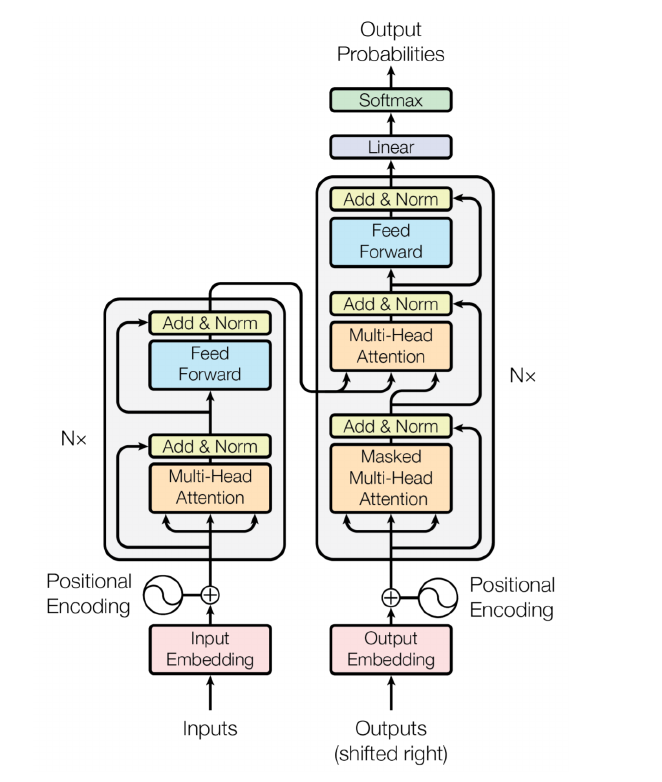
\includegraphics[width=0.85\textwidth]{images/chap3/transformer_arch.png}
	\caption[نمایی کلی از معماری ترنسفورمر]
	{
		نمایی کلی از معماری ترنسفورمر
		\cite{transformer}
	}
	\label{fig:chap3:transfoermer_overview}
\end{figure}

\subsection{کدگذار و کدگشا}
قسمت کدگذار ترنسفورمر از یک 
\trans{پشته}{Stack}
از چندین لایه یکسان تشکیل شده است که هر لایه خروجی خود را به عنوان ورودی به لایه بعدی تحویل می‌دهد. در هر لایه پشته کدگذار دو بلوک وجود دارد. بلوک اول یک مکانیزم 
\trans{خودتوجه چندسر}{Multi-Head Self-Attention}
است و بلوک دوم نیز یک شبکه عصبی 
\trans{پیشرو}{Feed-Forward}
\trans{تمام متصل}{Fully connected}
است که مستقل از مکان عمل می‌کند. در ضمن در هر بلوک نیز از 
\trans{اتصالات باقی‌مانده}{Residual Connection}
و 
\trans{هنجارساز لایه}{Layer Normalization}
استفاده می‌شود.

زیر شبکه کدگشای ترنسفورمر نیز مانند کدگذار دارای چندین لایه است با این تفاوت که هر لایه دارای سه بلوک است. بلوک اول و بلوک سوم کدگشا دقیقا مانند بلوک های اول و دوم کدگذار هستند. بلوک میانی اما در واقع نقش اتصال کدگذار و کدگشا را دارد و به وسیله یک توجه چند سر، مکانیزم توجه را روی خروجی آخرین لایه کدگذار انجام می‌دهد. در ضمن یک تفاوتی که در بلوک اول کدگذار با کدگشا وجود دارد این است که عمل توجه به خود در کدگشا صرفا بر روی ورودی‌های قبل از توکنی که قصد توجه دارد انجام می‌شود.


\subsection{مکانیزم توجه در ترنسفورمر}

\subsubsection{تعمیم مکانیزم توجه}
در این پژوهش مکانیزم توجه به شکل تعمیم یافته‌ای ارائه شده است. در واقع در مکانیزم توجه تعمیم یافته سه جزء اساسی بردار 
\trans{پرس و جو}{Query}
و یک جفت بردار‌های کلید-مقدار برای هر توکن در نظر گرفته می‌شوند. بردار خروجی مکانیزم توجه، حاصل جمع‌ وزن‌دار بردارهای مقدار  توکن‌های مورد توجه می‌باشد که این وزن‌ها خود تابعی از بردار 
پرس و جوی توکن در حال توجه و بردارهای کلید توکن‌های مورد توجه می‌باشند.

در روند پیاده‌سازی مکانیزم توجه در مدل ترنسفورمر از تابع ضرب داخلی به عنوان تابع محاسبه‌گر امتیاز مشابهت بردار‌های پرس و جو و کلید استفاده شده است.
سپس با اعمال تابع 
\trans{بیش‌نرم}{Softmax}
 روی تمامی امتیاز‌های مشابهت متعلق به توجه یک بردار پرس و جو بر روی مجموعه ای بردارهای کلید، وزن مربوطه ترکیب خطی مکانیزم توجه محاسبه می‌گردد. در نهایت از آن‌جایی که به ازای مقادیر بزرگ 
$d_k$
که اندازه بردار کلید است، حاصل ضرب داخلی بسیار بزرگ می‌شود و خروجی تابع 
بیش‌نرم
به گونه‌ای می‌شود که مشتق بسیار ضعیفی به عقب باز‌ می‌گردد، جهت رفع این مشکل، امتیازات قبل از اعمال 
بیش‌نرم
تقسیم بر 
$\sqrt{d_k}$
می‌شوند. جهت درک بهتر این عملیات شکل
\ref{fig:chap3:transformer_attention}
 آورده شده است.

\begin{figure}[h]
	\centering
	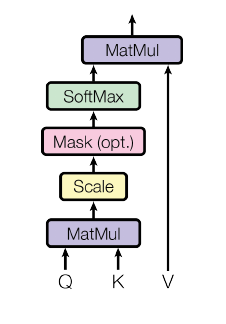
\includegraphics[width=0.3\textwidth]{images/chap3/transformer_attention.png}
	\caption[نمایی از مکانیزم نوجه در مدل ترنسفورمر]
	{
		نمایی از مکانیزم توجه در مدل ترنسفورمر
		\cite{transformer}
	}
	\label{fig:chap3:transformer_attention}
\end{figure}

\subsubsection{مکانیزم توجه چندسر}

نکته جالب توجه دیگر در معماری ترنسفورمر مکانیزم توجه چندسر است. در مقاله این گونه بیان شده که به جای این که هر بار یک توجه با ابعاد بردار 
$d_{model}$
انجام بگیرد، می‌توان بردارهای پرس و جو، کلید و مقدار را با کمک شبکه‌های پیشرو قابل یادگیری به تعداد
$h$
فضای با ابعاد
$d_{model/h}$
تصویر کرد و سپس 
$h$
عمل توجه را روی این بردار‌های تصویر شده انجام داد و در نهایت حاصل این توجهات را با یکدیگر الحاق کرد. مکانیزم توجه چندسر به مدل اجازه می‌دهد تا همزمان بتواند به اطلاعاتی از فضاهای 
\trans{بازنمایی}{representation}
مختلفی توجه کند. به علاوه امکان موازی‌سازی بین این عملیات‌های توجه نیز فراهم است و از این حیث مدل دچار هزینه زمانی اضافی نمی‌شود. برای درک بهتر مکانیزم توجه چندسر شکل 
\ref{fig:chap3:transformer_multihead}
آورده شده است.
\begin{figure}[h]
	\centering
	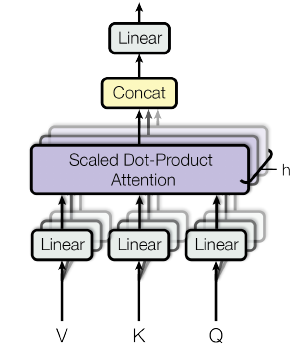
\includegraphics[width=0.4\textwidth]{images/chap3/transformer_multihead.png}
	\caption[نمایی از مکانیزم توجه چندسر در مدل ترنسفورمر]
	{
		نمایی از مکانیزم توجه چندسر در مدل ترنسفورمر
		\cite{transformer}
	}
	\label{fig:chap3:transformer_multihead}
\end{figure}


\subsubsection{موارد استفاده از توجه در ترنسفورمر}
مدل ترنسفورمر از مکانیزم توجه چندسر در سه موقعیت مختلف استفاده می‌کند:

\begin{itemize}
	\item 
	\textbf{توجه کدگشا به کدگذار}:
	در این بخش بردار‌های پرس و جو از لایه‌ی‌ قبلی کدگشا حاصل می‌شوند و بردارهای کلید و مقدار نیز از خروجی کدگذار به دست می‌آیند.
	
	\item 
	\textbf{توجه به خود کدگذار}:
	در این بخش تمامی بردارهای پرس و جو و کلید و مقدار از خروجی لایه قبلی کدگذار حاصل می‌شوند. هر توکن در هر مکانی در کدگشا می‌تواند به تمامی توکن‌ها (چه قبل و چه بعد از خود) توجه کند.
	
	\item
	\textbf{توجه به خود کدگشا}:
	این مورد مانند توجه به خود کدگشا است، با این تفاوت که هر توکن در کدگشا تنها می‌تواند به بردارهای مقدار و کلید توکن‌های قبل از خود توجه کند.
	
	
\end{itemize}

\subsection{شبکه پیشرو تمام متصل مستقل از مکان}
علاوه بر بلوک توجه، هر یک از لایه‌ها در کدگذار و کدگشا دارای یک بلوک شبکه عصبی تمام متصل پیشرو هستند. این شبکه به هر برداری در هر مکانی به صورت جدا و البته یکسان اعمال می‌شود (البته دقت شود که پارامتر‌های این شبکه‌های متصل لایه به لایه فرق می‌کنند). این شبکه یک شبکه با یک لایه مخفی است، اندازه بردارهای ورودی و خروجی آن ۵۱۲ می‌باشد و اندازه بردار حالت نهان آن هم ۲۰۴۸ است. کاربرد و فلسفه وجودی این شبکه در استخراج ویژگی از بردارهای حاصل از مکانیزم توجه است.


\subsection{
مکانیزم تعبیه
مکانی
}

از آنجایی که ساختار شبکه ترنسفورمر بازگشتی نمی‌باشد، بنابراین لازم است تا مکانیزمی جهت تزریق اطلاعات موقعیت مکانی کلمات دنباله نسبت به یکدیگر به مدل طراحی شود. به منظور حل این چالش در مدل ترنسفورمر برداری به نام بردار 
\trans{تعبیه}{Embedding}
 مکانی در نظر گرفته شده است که بنابر رابطه
\ref{eq:positional_embedding}
به دست می‌آید.

\begin{align} \label{eq:positional_embedding}
PE_{(pos, 2i)} = sin(pos/10000^{2i/d_{model}}) \\  \nonumber
PE_{(pos, 2i+1)} = cos(pos/10000^{2i/d_{model}}) 
\end{align}

این بردار تعبیه مکانی با اندازه 
\lr{$d_{model}$}
 به ازای هر توکن با مکان مختلف که متغیر
\lr{pos}
می‌باشد تعریف می‌شود. در نهایت بردار تعبیه مکانی با بردار تعبیه کلمه جمع خواهد شد.

\subsection{علت اهمیت به معماری ترنسفورمری}
ترنسفورمر‌ها به علت توانایی موازی‌سازی عملیات‌های خود در هنگام آموزش نسبت به شبکه‌های بازگشتی، سریعتر آموزش می‌بینند. از طرفی وجود عملیات توجه به خود چه در کدگذار و چه در کدگشا نیز خود عاملی برای تقویت این مدل نسبت به مدل‌های بازگشتی استفاده کننده از توجه شده است و به صورت خاص به نظر می‌رسد که وجود این توجه به خود برای مساله گفتگو بسیار موثرتر از وجود مکانیزم توجه بدون توجه به خود است.

\section{نهضت انتقال یادگیری در پردازش زبان}
تولد 
\trans{الگوواره}{paradigm}
 انتقال یادگیری را می‌توان مترادف با به وجود آمدن شبکه‌های غول آسایی نظیر
\LR{AlexNet}
و
\LR{VGG}
که بر روی دادگان عظیم تصویری آموزش یافته‌اند در نظر گرفت. محققان حوزه یادگیری عمیق و بینایی ماشین، با آموزش این مدل‌ها روی دادگان عظیم در پی این بودند که بتوانند بازنمایی‌های مناسبی از تصاویر به دست آورند؛ به نحوی که در روند حل مسائل دیگر بتوانند از آن‌ها به عنوان ویژگی‌ استفاده کنند. 

در حوزه متن اما اولین نمونه از انتقال یادگیری را می‌توان مدل معروف 
\lr{word2vec}
 ارائه شده توسط میکولوف در سال ۲۰۱۳ دانست
\cite{word2vec_paper}.
به این صورت که وظیفه حدس زدن کلمات اطراف یک کلمه توسط یک شبکه با یک لایه مخفی بر روی دادگان بسیار آموزش دیده شده و بازنمایی حاصل از آن شبکه به عنوان بازنمایی هر کلمه مدنظر قرار گرفت. پس از عرضه مدل 
\lr{word2vec}
مرز‌های دانش در بسیاری از مسائل پردازش زبان، بسیار فراتر از حد فعلی خود رفتند و این مدل کارایی خود را به نمایش گذاشت. اما از آن‌جایی که نقطه قوت این مدل از منظر انتقال یادگیری مورد توجه واقع نشد،‌ مسئله انتقال یادگیری نیز در حوزه پردازش زبان چند سال به خواب عمیقی فرو رفت تا آن که در سال ۲۰۱۸ مدل 
\lr{ELMO}
انتشار یافت
\cite{elmo_paper}.

توضیح آن‌که با وجود این که شبکه‌هایی نظیر 
\lr{word2vec}
برای هر کلمه یک بردار بازنمایی مناسب تولید می‌کردند اما وجود کلمات چند معنایی مانند "شیر" و یا "بستر" (که با آن که یک معنا دارد اما  در جمله‌ می‌تواند به معنای بستر خواب یا بستر رودخانه باشد) محققین را به این فکر انداخت که بازنمایی یک کلمه بایستی تابعی از محتوایی که آن کلمه در آن قرار گرفته نیز باشد.  به فرض مثال بازنمایی کلمه "شیر" در دو عبارت "من شیر را خوردم" و یا "شیر سلطان جنگل است" بایستی متفاوت بوده و تابعی از جمله باشد. 

به طور اجمالی مدل 
\lr{ELMO}
از دو شبکه 
\lr{LSTM}
چند لایه تشکیل شده است که یکی از آن‌ها وظیفه 
\trans{مدل زبانی}{Language Model}
را از سمت چپ و دیگری نیز وظیفه 
مدل زبانی
را از سمت راست روی دادگان متنی آموزش می‌بینند. 
\footnote{
توضیح آن که یادگیری وظیفه مدل زبانی از دو سمت باعث می‌شود تا بازنمایی بهتری برای کلمات به وجود بیاید. برای مثال دو عبارت "من شیر جنگل را دیدم" را با "من شیر را همراه با کیک میخورم" مقایسه کنید. در صورتی که تنها از یک شبکه بازگشتی استفاده کنیم و جمله را از راست به چپ به شبکه بازگشتی ورودی بدهیم بازنمایی کلمه شیر در هر دو عبارت یکی خواهد بود.
}
در مرحله بعد، در صورتی که بخواهند از این شبکه به عنوان نقطه شروع و یا شبکه استخراج ویژگی از کلمات برای یک وظیفه دیگر استفاده کنند، ترکیب خطی قابل یادگیری از بازنمایی کلمات در لایه‌های مختلف هر دو
\lr{LSTM}
را به عنوان بازنمایی آن کلمه در نظر می‌گیرند. برای درک بهتر معماری ELMO در شکل 
\ref{fig:chap3:elmo_arch}
به نمایش درآمده است.

\begin{figure}[h]
	\centering
	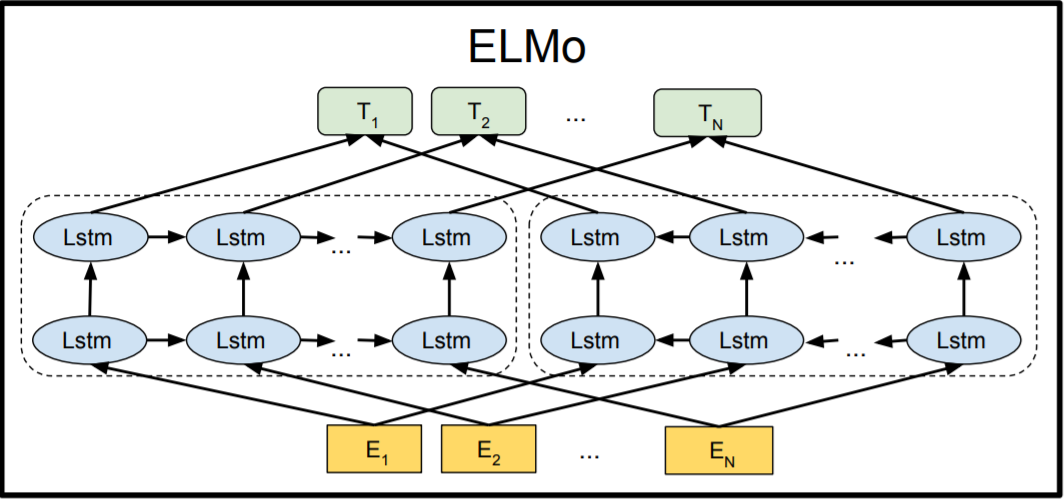
\includegraphics[width=0.8\textwidth]{images/chap3/elmo_arch.png}
	\caption{
		نمایی از معماری مدل المو
	}
	\label{fig:chap3:elmo_arch}
\end{figure}

 با ظهور مدل المو مرز‌های دانش در مسائل پردازش زبان گسترش پیدا کردند و امتیاز بهترین مدل‌ها در مسائل گوناگون پردازش زبان بهبود یافت. با این وجود به دلیل این که المو یک شبکه بازگشتی محسوب می‌شد، مشکلات شبکه‌های بازگشتی از قبیل توانایی کمتر در موازی‌سازی و همچنین انفجار یا ناپدید شدن گرادیان، در المو نیز وجود داشت.  

\subsection{مدل برت}
پس از ارائه معماری ترنسفورمر، توجهات در حوزه پردازش زبان از معماری‌های بازگشتی به معماری‌های ترنسفورمری معطوف گشت و در اغلب مسائل مهاجرت از معماری های بازگشتی به معماری‌‌ها نو شکل گرفت. 
طبعا این مهاجرت محققان این حوزه را نیز به این فکر انداخت تا مدلی با معماری ترنسفورمری و با کارکرد مشابه با المو ارائه دهند. سرانجام این ایده، منجر به انتشار مدل برت در سال ۲۰۱۹ گردید
\cite{bert}
.

مدل برت از لحاظ ساختاری، یک پشته کدگذار ترنسفورمری محسوب می‌شود. 
\footnote{در واقع ترنسفورمری است که تنها قسمت کدگذار را داراست و فاقد قسمت کدگشا است.}
هدف مدل برت مشابه المو به دست آوردن یک بازنمایی از طریق آموزش روی دادگان فراوان متنی بدون برچسب است. مزیت ساختاری برت بر المو را نیز می‌توان اولا در سرعت بالاتر و آموزش راحت شبکه‌ ترنسفورمری نسبت به شبکه بازگشتی دانست و از آن مهم‌تر امکان توجه توامان
\trans{دوطرفه}{Bidirectional}
 در هر کلمه نسبت به محتوای سمت چپ و راست آن دانست. در واقع در مدل برت بردار بازنمایی یک کلمه می‌تواند به کلمات سمت راست و چپ خود همزمان توجه کند در حالی که در مدل المو ما با دو شبکه بازگشتی مواجه هستیم که هر یک سعی دارند به طور غیرتوام توجه بردار بازنمایی کلمه را به سمت چپ و راست معطوف کنند. 
 
 در مقاله برت دو طرح اساسی مطرح شده است. طرح اول، چگونگی پیش آموزش شبکه برت و طرح دوم نیز چگونگی تنظیم آن روی وظایف مختلف پردازش زبان است.
 
 \subsubsection{چگونگی پیش‌آموزش برت}
 به منظور پیش آموزش شبکه برت، دو وظیفه 
 \trans{مدل زبانی پوشیده}{Masked-Language-Model}
 و 
 \trans{تشخیص جمله بعدی}{Next Sentence Prediction}
 انتخاب شده اند.
در مسئله مدل زبانی پوشیده، بر خلاف مسئله مدل زبانی عادی که در آن هدف یادگیری
\trans{توزیع احتمال}{Probability Distribution}
کلمه از روی کلمات قبلی‌اش است، هدف یادگیری توزیع اجتمال یک کلمه از روی کلمات قبل و بعد از خودش است. طبیعی است که با توجه به اهتمام برت بر به دست آوردن یک بازنمایی دوطرفه توامان وظیفه مدل زبانی پوشیده جهت نیل به این هدف بسیار موثر تر از وظیفه مدل زبانی عادی است. در هنگام پیش آموزش برت با وظیفه مدل زبانی پوشیده، به تصادف ۱۵ درصد از کلمات دنباله با توکن 
\lr{MASK}
تعویض می‌شوند و مدل بایستی بتواند که کلمه اول توکن‌های پوشیده شده را تشخیص دهد. 

با این که آموزش روی وظیفه مدل زبانی پوشیده به برت کمک می‌کند برای هر کلمه بازنمایی موثری بیابد اما برت برای انجام برخی مسائل پردازش زبان نیاز به ارائه بازنمایی مناسبی از جملات
و همچنین کشف رابطه بین جملات مختلف،
 نیز دارد. به این منظور، برت پس از پیش آموزش مدل زبانی پوشیده، روی وظیفه حدس جمله بعدی نیز آموزش می‌بیند. صورت این مساله این شکلی است که جمله A از دادگان آموزشی انتخاب می‌شود. سپس به احتمال پنجاه درصد جمله پس از A به عنوان جمله B انتخاب می‌شود و یا به احتمال باقی مانده پنجاه درصد یک جمله تصادفی به عنوان جمله B انتخاب می‌شود. سپس مدل بایستی این که آیا جمله B جمله بعدی جمله A است یا خیر را حدس بزند. 

 در پیاده‌سازی برت، هنگام ورود یک رشته در ابتدای آن یک توکن
\lr{[CLS]}
اضافه می‌شود که بردار بازنمایی حاصل آن از شبکه برت، بردار بازنمایی جمله را ارائه می‌دهد و در وظیفه تشخیص جمله بعدی، یک لایه
\lr{Softmax}
روی بردار بازنمایی
\lr{[CLS]}
اضافه گشته و احتمال خواسته شده را به دست می‌آورد. همچنین در پایان هر جمله نیز توکن
\lr{[SEP]}
اضافه می‌شود که جهت نشان دادن اتمام جمله ها به مدل به کار می‌رود. علاوه بر این، بردار
\trans{تعبیه قطعه‌ای}{Segment Embedding}
قابل یادگیری نیز با دو مقدار مختلف به دو جمله اول و دوم اعمال می‌شود. در واقع برت دارای سه مکانیزم تعبیه مکانی، قطعه‌ای و کلمه‌ای است که به ترتیب بر رشته ورودی اعمال می‌شود. جهت درک بهتر این تعبیه‌سازی‌ها، شکل
\ref{fig:chap3:bert_embeddings}
 آورده شده است.

 \begin{figure}[h]
 	\centering
 	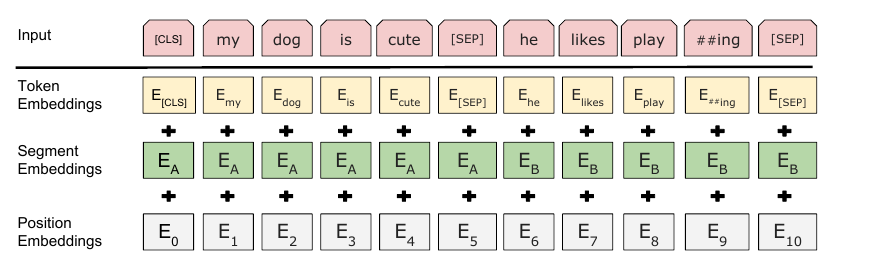
\includegraphics[width=1\textwidth]{images/chap3/bert_embeddings.png}
 	\caption[نمایی از انواع تعبیه در مدل برت]
 	{
 		نمایی از انواع تعبیه در مدل برت
 		\cite{bert}
 	}
 	\label{fig:chap3:bert_embeddings}
 \end{figure}

حسن و مزیت مسائل پیش آموزش برت در این است که دادگان بی‌برچسب موردنیاز آن‌ها به آسانی قابل جمع آوری است و همین باعث شده است که در طی دوره کوتاهی مدل برت 
توسط افراد مختلف
برای زبان‌های دیگر (از جمله فارسی) نیز آموزش یافته و در اختیار عموم قرار گیرد
\cite{parsbert}.

\subsubsection{نحوه تنظیم برت برای وظایف مختلف}
در مقاله برت،‌ پس از مشخص‌شدن نحوه پیش آموزش این شبکه، معماری‌های پیشنهادی مبتنی بر برت برای حل بعضی از مسائل پردازش زبان نظیر تحلیل احساسات، تشخیص موجودیت‌های اسمی و پرسش و پاسخ ارائه شده است. رویکرد حل این مسائل با برت به این نحو است که معمولا لایه‌هایی جهت حل مساله مورد نظر به برت پیش آموزش یافته اضافه می‌شوند و معماری جدید (که برت پیش‌آموزش یافته حالا جزیی از آن است) روی مساله مورد نظر و دادگان برچسب‌دار آن تنظیم می‌شود. 

\subsection{مدل‌های پس از برت}
با این که با عرضه برت، یک انقلاب در حوزه پردازش زبان و مسائلش رخ داد و مرز‌های دانش بسیاری از مسائل با استفاده از معماری‌های مبتنی بر برت پیشرفت قابل توجهی را تجربه کردند؛ اما برت بی عیب و نقص نیست و راه‌حل تمامی مسائل پردازش زبان نیز محسوب نمی‌شود. به دلیل ضعف‌های نسبی برت و همچنین موفقیت چشم‌گیر آن بسیاری از پژوهشگران نیز در ادامه کوشیدند تا شبکه‌های از پیش آموزش یافته دیگری که بر پایه معماری ترنسفورمر باشند، را پیش آموزش داده و عرضه کنند.
از مهم‌ترین این شبکه‌ها بایستی به سری شبکه‌های 
\lr{GPT}
اشاره کرد که با انتشار خود، باعث پیشروی مرز‌های دانش در حوزه مسائل تولید زبانی شدند و حتی با خروجی‌های شگفت انگیز خود همگان را حیرت زده کردند
\cite{gpt2_paper, gpt3_paper}.

و یا می‌توان به شبکه
\lr{Transformer-XL}
اشاره کرد که سعی دارد با اندکی تغییر در ساختار ترنسفومر، مشکل محدودیت برت 
(برت تنها می‌تواند متونی با حداکثر طول ۵۱۲ توکن را کد کند)
در طول متون ورودی را حل کند
\cite{DBLP:journals/corr/abs-1901-02860}.

با وجود همه این پیشرفت‌ها و حتی به راه افتادن رقابت بین شرکت‌های بزرگ دنیا بر سر آموزش دادن یک مدل بزرگتر و با تعداد پارامتر بیشتر، اما به نظر می‌رسد در طول این رشد و رقابت روزافزون بین مدل‌های از پیش آموزش یافته، غفلتی نسبت به بخشی از ایده اصلی ترنسفورمر‌ها صورت گرفته است. تمامی شبکه‌های از پیش آموز‌ش‌یافته ارائه شده تا قبل از مدل برت، را می‌توان تنها متشکل از یک پشته کدگذار معماری ترنسفورمر دانست. حتی تحت تاثیر این اتفاق، معماری‌های ارائه شده مبتنی بر این شبکه‌های از پیش آموزش یافته برای مسائل با ذات دنباله به دنباله نظیر مکالمه نیز، حالت دنباله به دنباله خود را از دست دادند و به صورت مدل زبانی مدل شدند
\cite{zhang2019dialogpt}.


\subsection{مدل بارت}
در حالی که بسیاری از محققین در حال صرف هزینه و تمرکز بر روی ایجاد مدل‌های تک پشته‌ای بودند، معماری دنباله به دنباله با عرضه مدل 
\trans{بارت}{Bart}
دوباره مورد توجه واقع شد. مدل بارت از لحاظ ساختاری یک ترنسفورمر کامل (پشته کدگذار به همراه پشته کدگشا) است. این مدل بر روی مساله بازسازی متن اصلی از روی متن 
\trans{خراب‌شده}{corrupted}
پیش آموزش می‌بیند و جهت بهینه‌سازی سعی در کمینه‌ کردن 
\trans{منفی لگاریتم بیشینه‌نمایی}{Negative Log Likelihood}
رشته خروجی می‌کند
\cite{lewis2019bart}.
 
 به صورت دقیق‌تر در طی فرآیند پیش‌‌‌ آموزش بارت، ابتدا داده‌‌ها (جملات) متنی بی برچسب توسط 
\trans{تابع نوفه‌ای‌ساز}{Noising Function}
دستکاری و به اصطلاح خراب می‌شوند. سپس این جملات خراب به مدل بارت ورودی داده می‌شود و بارت بایستی با استفاده از ساختار دنباله به دنباله خود، جمله اصلی را بازسازی کند. احتمال بازسازی جمله اصلی نیز از طریق محاسبه درست‌نمایی آن در کدگشای بارت حاصل می‌شود. برای درک بهتر این موضوع شکل
\ref{fig:chap3:bart_pretraining}
آورده شده است. در ضمن در هنگام تنظیم بارت روی وظایف دنباله به دنباله دیگر نظیر پرسش و پاسخ، متن پرسش به صورت سالم به قسمت کدگذار ورودی داده شده و از کدگشا انتظار می‌رود تا بتواند متن پاسخ را تولید کند.

 \begin{figure}[h]
	\centering
	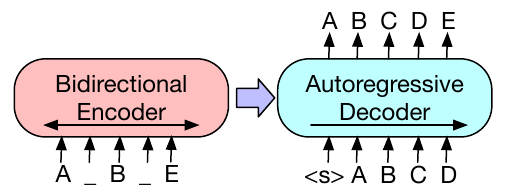
\includegraphics[width=0.6\textwidth]{images/chap3/bart_seq2seq.png}
	\caption[نمایی از نحوه پیش آموزش بارت]
	{
		نمایی از نحوه پیش آموزش بارت
		\cite{lewis2019bart}
	}
	\label{fig:chap3:bart_pretraining}
\end{figure}

ذکر این نکته ضروری است که بارت در پیش آموزش خود از پنج تابع آشوبگر زیر استفاده می‌کند:

\begin{itemize}
	\item 
	\textbf{
\trans{پوشاندن توکن‌ها}{Token Masking}	
}

به مانند مسئله پیش آموزش برت، در این جا نیز، توکن‌هایی به صورت تصادفی انتخاب شده و با نماد
\lr{\_}
جایگزین می‌شوند.

\item 
\textbf{
	\trans{حذف توکن‌ها}{Token Deletion}	
}

این تابع مانند مورد قبل است با این فرق که توکن انتخاب شده حذف می‌گردد و هیچ نمادی جای آن را نمی‌گیرد.

\item 
\textbf{
	\trans{پر یا خالی کردن متن}{Text Infilling}	
}

این تابع آشوبگر محدوده‌ای متن را انتخاب کرده (با طول توکن‌ دلخواه صفر، یک، دو و ...) سپس جای آن محدوده نماد 
\lr{\_}
را می‌گذارد.

\item 
\textbf{
	\trans{جایگردی جملات}{Sentence Permutation}	
} 

	این تابع آشوبگر متن را بر اساس علائم نگارشی خاتمه دهنده جمله نظیر نقطه، به دو قسمت تقسیم می‌کند و جای قسمت اول و دوم را عوض می‌کند.
\item 
\textbf{
	\trans{دوران متن}{Document Rotation}	
} 	

این تابع آشوبگر یک توکن را به تصادف انتخاب می‌کنند و متن را به گونه‌ای دوران می‌دهد که این توکن، آغازگر متن باشد.
\end{itemize}

جهت درک بهتر این توابع آشوبگر شکل
\ref{fig:chap3:bart_noising_function}
آورده شده است.
 \begin{figure}[h]
	\centering
	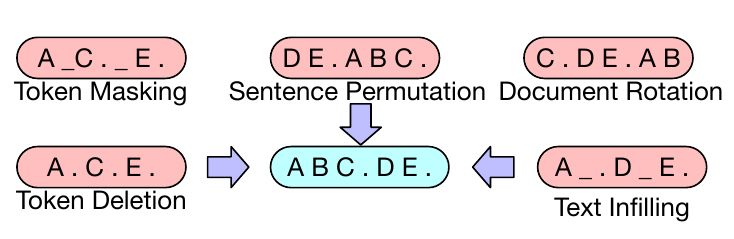
\includegraphics[width=0.6\textwidth]{images/chap3/bart_noising_function.png}
	\caption[نمایی از توابع نوفه‌ای‌ساز مورد استفاده در بارت]
	{
		نمایی از توابع نوفه‌ای‌ساز مورد استفاده در بارت
		\cite{lewis2019bart}
	}
	\label{fig:chap3:bart_noising_function}
\end{figure}

مدل بارت بر روی مسائل دنباله به دنیاله‌ای نظیر تنظیم ترجمه ماشینی و خلاصه‌سازی تنظیم شده و عملکرد موثری را ارائه داده است. به طوری که بهترین مدل‌های خلاصه‌سازی تا به اکنون، مدل‌های مبتنی بر بارت هستند. 

\section{شگرد عصاره‌گیری دانش 
}
ظهور شبکه‌ها و مدل‌های از پیش آموزش دیده با مقیاس بزرگ، با آن که پیشرفت قابل توجهی را در مسائل مختلف پردازش زبان رقم زدند؛ اما استفاده از آنان برای پژوهشگران چندان ساده نبود.
مقیاس بالا این شبکه و داشتن تعداد پارامتر‌های زیاد (از چند صد میلیون تا چند ده میلیارد حتی) مانع از استفاده موثر از آنان چه در زمان آموزش و تنظیم بر روی یک وظیفه و چه در زمان 
\trans{استقرار}{Deployment}
در جایگاه کاربردی می‌شود. در واقع تعامل با این مدل‌ها مستلزم در اختیار داشتن سخت‌افزار‌های پیشرفته است. در هنگام آموزش ورودی دادن یک
\trans{دسته}{batch}
از دادگان به این شبکه‌ها و خروجی گرفتن از آن‌ها مستلزم داشتن سخت‌افزار‌های با حافظه انبوه است و در هنگام استقرار به علت نیاز به پاسخ‌گیری 
\trans{بی‌درنگ}{Real-Time}
بایستی سخت‌افزاری فراهم بشود که بتواند با قدرت محاسباتی بالای خود به سرعت دادگان ورودی را از چند صدلایه سلول‌های عصبی عبور داده و خروجی را تولید نماید. 

در این هنگام بود که توجه پژوهشگران به ایده عصاره‌گیری دانش
که در سال ۲۰۱۵ ارائه یافته بود، معطوف شد
\cite{hinton2015distilling}.
عصاره گیری دانش شگرد فشرده‌سازی است که در آن یک مدل کوچک‌تر (که مدل دانش‌آموز نامیده می‌شود) آموزش می‌بیند تا رفتار مدل‌بزرگ‌تر (که مدل معلم نامیده‌می‌شود) را تقلید و بازتولید کند
\cite{hinton2015distilling}.

در فرآیند یادگیری بانظارت، مدل معمولا به گونه‌ای آموزش می‌بیند که بتواند توزیع احتمالاتی خود در مورد برچسب نمونه‌ها را به توزیع 
\trans{تک داغ}{One-Hot}
برچسب‌ آن‌ها نزدیک کند. این مهم معمولا از طریق کمینه‌سازی تابع هزینه
\trans{انتروپی متقاطع}{Cross-Entropy}
صورت می‌گیرد. جهت یادآوری آنتروپی متقاطع رابطه
\ref{eq:cross_entropy}
 آورده شده است که در آن $o$ بردار احتمالاتی تخمین زده شده توسط شبکه عصبی و $y$ نیز بردارتک فعال برچسب داده مورد نظر است.


\begin{align} \label{eq:cross_entropy}
L(y, o) = \sum_{i}^{} y_i\:log\,o_i
\end{align}

اما در فرآیند عصاره‌گیری، به طور اجمالی مدل دانش آموز از طریق کمینه‌کردن تابع هزینه عصاره‌گیری روی بردار‌های احتمالاتی خروجی مدل معلم آموزش می‌بیند. رابطه این تابع هزینه در رابطه
\ref{eq:cross_distill}

آورده شده است. در این رابطه $t$ بردار احتمالاتی حدس زده شده توسط مدل معلم و $s$ نیز بردار احتمالاتی حدس زده شده توسط مدل دانش آموز است.

\begin{align} \label{eq:cross_distill}
L_{ce} = \sum_{i}^{} t_i\:log\,s_i
\end{align}

اولین تلاش جدی در زمینه عصاره‌گیری از مدل‌های زبانی از پیش آموزش دیده را می‌توان مدل 
\lr{DistilBert}
دانست
\cite{sanh2019distilbert}.
این مدل سعی کرده است دانش مدل برت را 
تا حد ممکن به یک مدل با ساختار معماری مشابه برت ولی تعداد  لایه‌ها و پارامتر‌های کمتر انتقال دهد. در نهایت این مدل کوچکتر با تعداد پارامتر معادل ۶۰ درصد تعداد پارامتر‌های مدل برت اصلی،
توانسته به طرز حیرت آوری حدود ۹۷ درصد از عملکرد برت را روی وظایف مختلف حفظ کند. 

در ادامه در پژوهش دیگری، مدل‌های عصاره‌گرفته‌شده دیگری از برت تحت عنوان برت‌های مینیاتوری ارائه گردید
\cite{turc2019well}.
این مدل‌ها ابتدا خود به تنهایی بر روی دادگان بی برچسب پیش آموز یافته و سپس بر روی وظیفه گیری عصاره‌گیری برت، تنظیم شده‌اند. این مدل‌های برت مینیاتوری در دو تنظیمات مختلف 
با تعداد لایه‌های دو، چهار، شش، هشت، ده، دوازه و با اندازه حالت نهان ۱۲۸ و ۲۵۶ و ۵۱۲ و ۷۶۸ ارائه شده‌اند. کوچکترین این مدل‌ها که دو لایه با اندازه حالت نهان ۱۲۸ دارد، با تعداد پارامتر معادل ۴ درصد تعداد پارامترهای برت اصلی، توانسته است حدود ۶۰ درصد از عملکرد برت‌ اصلی را روی وظایف درک زبانی حفظ کند
\cite{turc2019well}.

استفاده از این برت‌های مینیاتوری در موقعیت‌هایی که محدودیت‌های سخت افزاری وجود دارد، می‌تواند به شدت موثر واقع شود.

\section{معیارهای سنجش تولید متن}

% \subsection{مقدمه}
هنگامی که گپ‌زن پاسخ‌ خود را تولید کند، بایستی مکانیزمی برای سنجش کیفیت متن تولید شده وجود داشته باشد تا بتوان میزان موفقیت مدل در امر تولید متن را بررسی کرد. روش‌های سنجش کیفیت متن‌های تولید شده را 
می‌توان به دو دسته‌ روش‌های ذهنی و عینی تقسیم کرد. در روش‌های ذهنی، عوامل با مشاهده متن تولید شده آن را امتیازدهی می‌کنند و کیفیت یک مدل یا چند مدل به وسیله میانگین امتیازات دریافت شده توسط عوامل انسانی مشخص می‌شود. بدیهی است که انجام نظرسنجی انسانی کاری با هزینه بالا (چه هزینه مادی و چه هزینه زمانی) محسوب می‌شود و از طرفی گزینش عوامل انسانی نیز در این مورد باید به دقت صورت گیرد. برای مثال در زمینه سنجش کیفیت متن انگلیسی شده نمی‌توان از هر عامل انسانی فارسی زبانی در سنجش آن مدل نظرخواهی کرد؛ و بایستی از عوامل انگلیسی زبانی که بر آن زبان تسلط دارند استفاده شود. از طرفی دیگر حتی در صورت استفاده از عوامل خبره، باز هم نمی‌توان امتیازهای کسب شده توسط دو مدل مختلف که توسط دو فرد مختلف عرضه شده اند را بررسی کرد؛ چرا که این مدل‌ها هر کدام در دو جامعه انسانی گوناگون مورد ارزیابی قرار می‌‌گیرند و شرایط محیطی برای آن‌ها یکسان نخواهند بود. 

در چنین شرایطی است که لزوم وجود یک معیار عینی تمام خودکار احساس می‌شود. معیارهای عینی معیارهای هستند که می‌توان  آن‌ها را به صورت خودکار و مستقل از عامل انسانی محاسبه نمود. البته در اغلب موارد می‌توان عیب‌هایی را به معیارهای عینی مطرح شده در حوزه تولید زبانی مطرح نمود، چرا که اغلب این معیارها نمی‌توانند مکانیزمی جامع و کامل را برای کیفیت مدل در امر تولید زبانی مطرح کنند. در ادامه سه معیاری که در این پژوهش به عنوان معیارهای سنجش تولید پاسخ مدل گپ‌زن برگزیده شده‌اند معرفی خواهند شد. 

\subsection{سرگشتگی}
\trans{سرگشتگی}{Perplexity}
 در واقع نشان می‌دهد که مدل مورد سنجش، به جمله صحیح هدف چه احتمالی را نسبت دهد و برای این که طول جملات هم در این محاسبات موثر نشوند در رابطه از طول جملات استفاده می‌کند تا معیاری نرمال شده بر حسب طول جمله ارائه دهد. در صورتی که فرض شود جمله هدف
$W$
جمله ای به طول 
$N$
باشد که خود متشکل از کلمات
$w_1$ 
تا
$w_n$
باشد، سرگشتگی طبق رابطه
\ref{eq:perplexity}
 می‌تواند محاسبه شود. در این رابطه 
 $p(w_1, w_2, ..., w_n)$
 احتمالی است که مدل تولیدگر متن به جمله 
 $W$
 نسبت می‌دهد. 

\begin{gather} \label{eq:perplexity}
PP(W) = p(w_1, w_2, ..., w_n)^{-1/N}
\end{gather}

که در این رابطه 
$p(w_1, w_2, ..., w_n)$
احتمالی است که مدل تولیدگر متن به جمله 
$W$
نسبت می‌دهد. 

از منظر احتمالاتی نیز می‌توان سرگشتگی را ضریب انشعاب متوسط یک مدل در فرآیند پیش‌بینی یک نمونه دانست.

\subsection{
امتیاز
\lr{F1}
}

رایج‌ترین رویکرد در ارائه معیار برای سنجش کیفیت متن تولید شده نامزد نسبت به متن مرجع،‌ شمردن 
$N$
تایی‌های مشترک بین دو متن نامزد و مرجع است. 

به صورت نمادی، در صورتی که 
$S_{x}^{n}$
و
$S_{\hat{x}}^{n}$
لیستی از چندتایی‌های حاضر در جملات مرجع 
$x$
و جمله نامزد 
$\hat{x}$
باشند، در این صورت دو امتیاز صحت 
$ (P_n) $
و فراخوانی 
$(R_n)$
مطابق رابطه
\ref{eq:exact_matching}
 محاسبه می‌شوند.

\begin{align}\label{eq:exact_matching}
 P_n = \frac{
\sum_{w \in S_{\hat{x}}^{n} }^{} \mathbb{I}[w \in S_{x}^{n}]
}{|S_{\hat{x}}^{n}|}  \\ \nonumber \\ \nonumber
 R_n = \frac{
	\sum_{w \in S_{x}^{n} }^{} \mathbb{I}[w \in  S_{\hat{x}}^{n}]
}{|S_{x}^{n}|}
\end{align}

سپس بر طبق 
$P_n$
و
$R_n$
می‌توان امتیاز 
$F_n$
را تعریف کرد که مطابق رابطه
\ref{eq:fscore}
 محاسبه می‌شود.

\begin{align}\label{eq:fscore}
F_n=2\times \frac{P_n.R_n}{P_n+R_n}
\end{align}

هر چه قدر پارامتر 
$n$
مقدار بیشتری داشته باشد، معیارهای 
$P_n$
و
$R_n$
و
$F_n$
معیارهای سخت‌گیرانه‌تر و تا حدی دقیق‌تر خواهند بود. معیار
$F_1$
نیز در واقع به بررسی هم پوشانی یک‌تایی‌ها و کلمات مشترک جمله نامزد و جمله مرجع می‌پردازد. این معیار در قسمت ارزیابی بیشتر پژوهش‌های مسئله نیز به عنوان یک سنجه به کار می‌رود. 


\subsection{امتیاز برت}

یکی از مشکلات واضح معیارهای بناشده بر همپوشانی چندتایی های مشترک بین متن مرجع و تولید‌شده،‌ عدم توجه به شباهت‌ معنایی (فارغ از همپوشانی دقیق عبارات) بین متن مرجع و متن تولید شده است. برای مثال اگر در وظیفه تولید متنی، جمله مرجع یک نمونه آموزشی جمله "من روز جمعه خودرویی نو خریدم" باشد و مدل پس از آموزش، جمله "اینجانب ظهر آدینه ماشینی جدید معامله کردم" را تولید کند، معیارهای بنا شده بر همپوشانی مانند
\lr{F1}
و یا
\lr{BLEU}
میزان شباهت این دو جمله را (علی رغم این که معنای کاملا یکسان دارند) صفر تشخیص می‌دهند. 

به منظور رفع این چالش در سال ۲۰۲۰ معیار جدیدی به نام 
\lr{BERTScore}
پیشنهاد شد
\cite{bertscore_paper}.
به طور اجمالی به فرض داشتن
$x =  \langle x_1, ..., x_k\rangle$
و 
$\hat{x} = \langle \hat{x}_1, ..., \hat{x}_l \rangle$
به عنوان جملات مرجع و نامزد، رویکرد این معیار به این نحو است که ابتدا 
\trans{تعبیه زمینه‌ای}{Contexual Embedding}
کلمات جملات مرجع و نامزد را حساب می‌کند. 
این امر از طریق استفاده از شبکه قدرتمند برت صورت می‌گیرد؛ به این صورت که با ورودی دادن دو جمله 
$x$
و 
$\hat{x}$
به شبکه برت، مجموعه دنباله بردارهای 
$ \langle \mathbf{x}_1, ..., \mathbf{x}_k\rangle $
و
$ \langle \mathbf{\hat{x}}_1, ..., \mathbf{\hat{x}}_k\rangle $
به عنوان بردارهای بازنمایی کلمات این جمله منظور می‌شوند.
سپس میزان تناظر دو به دو این کلمات حاضر در جملات مرجع و نامزد به وسیله محاسبه شباهت کسینوسی بردارهای تعبیه‌ی این کلمات حساب می‌شوند. حال به منظور محاسبه معیارهای صحت و فراخوانی، برای هر یک از کلمات حاضر در جملات مرجع و نامزد، کلمه متناظر از جمله متقابل تعیین می‌شود. این کلمه، کلمه‌ای است که بیشترین شباهت کسینوسی را با کلمه مورد نظر دارد. حال میزان صحت و فراخوانی ازطریق محاسبه میانگین وزن‌دار شباهت کسینوسی کلمات جملات مرجع و نامزد نسبت به کلمه متناظر خود حساب شوند. وزن‌های میانگین وزن دار مذکور رابطه‌ای عکس با تعداد جملاتی که کلمه در آن‌ها به کار رفته است دارد. نحوه محاسبه این وزن‌ها در رابطه 
\ref{eq:idf}
با فرض حضور 
$M$
جمله مرجع 
${x^(i)}^{M}_{i=1}$
آمده است.

\begin{align} \label{eq:idf}
idf(w) = -log \frac{1}{M} \sum_{i=1}^{M} \mathbb{I}[w \in x^{(i)}]
\end{align}

 این وزن‌ها کمک می‌کنند تا واژگان با تکرار فراوان ولی بار معنایی کم (نظیر حروف اضافه "را" یا "که") نقش کمتری در محاسبه میزان شباهت دو جمله با یکدیگر داشته باشند. روابط جزیی محاسبه امتیاز برت در روابط 
\ref{eq:bertsocre:R}
و
\ref{eq:bertsocre:P}
و
\ref{eq:bertsocre:F}
آمده اند.
\begin{align}\label{eq:bertsocre:R}
R_{BERT} = \frac{
\sum_{x_i \in x}^{} idf(x_i) \max_{\hat{x}_j \in \hat{x} } \mathbf{x}_i^\intercal \mathbf{\hat{x}}_j
}
{\sum_{x_i \in x}^{} idf(x_i) } \\ \nonumber \\ \label{eq:bertsocre:P} 
P_{BERT} = \frac{
	\sum_{x_i \in \hat{x}}^{} idf(x_i) \max_{x_j \in x } \mathbf{x}_i^\intercal \mathbf{\hat{x}}_j
}
{\sum_{\hat{x}_i \in \hat{x}}^{} idf(x_i) } \\ \nonumber \\ \label{eq:bertsocre:F} 
F_{BERT} = 2 \frac{P_{BERT} \dot{R_{BERT}}}{P_{BERT}+R_{BERT}}
\end{align}

جهت درک بهتر از رویکرد امتیاز برت، نمایی از نحوه عملکرد این معیار در شکل 
\ref{fig:chap3:bertscore}
آمده است.

 \begin{figure}[h]
	\centering
	\includegraphics[width=1\textwidth]{images/chap3/bert_fig.pdf}
	\caption[نمایی از نحوه محاسبه امتیاز برت]
	{
		نمایی از نحوه محاسبه امتیاز برت
		\cite{bertscore_paper}
	}
	\label{fig:chap3:bertscore}
\end{figure}

\section{جمع‌بندی}
در این فصل مبانی نظری راهکار پیشنهاد شده در فصل بعدی تشریح شدند. در ابتدا معماری ترنسفورمر که دلیل اصلی انقلابات اخیر در حوزه پردازش زبان است، با جزییات ارائه شد. در ادامه، نهضت انتقال یادگیری و شبکه‌های از پیش آموزش داده شده در پردازش زبان طبیعی مورد بررسی قرار گرفتند و در رابطه با سیر تحول آن‌ها و نکات مثبت و منفی آن بحث صورت گرفت. در ادامه شگرد عصاره‌سازی معرفی شد که می‌تواند در شرایطی که پژوهشگران با کمبود منابع سخت افزاری جهت آموزش مدل خود مواجه هستند، موثر واقع شود. در آخر معیارهایی که در این پژوهش جهت ارزیابی پاسخ‌های تولید شده توسط گپ‌زن استفاده می‌شوند ارائه شده و در مورد نقاط قوت و ضعف آن‌ها پرداخته شد.

در فصول آتی راهکاری پیشنهادی برای مساله گپ‌زن دانش بنیان مطرح شده و عملکرد مدل برآمده از این راهکار پیشنهادی سنجیده خواهد شد.
\chapter{راهکار پیشنهادی}\label{chap4}
\minitoc


\section{مقدمه}
پس از تعریف مساله و مرور پژوهش‌های پیشین مرتبط با آن و ارائه مبانی نظری، در این  فصل راهکاری پیشنهادی برای مساله گپ‌زن دانش بنیان طرح خواهد شد. این طرح شامل ارائه کلیات درباره دو بخش انتخاب دانش و تولید پاسخ است و در جزییات هر یک از این بخش‌ها نیز تشریخ می‌شود. اساس این راهکار پیشنهادی، با توجه به شرایط سخت افزاری در دسترس برای پیاده‌سازی آن، بر دو بخش انتخاب دانش و تولید پاسخ بنا شده است که تکیه هر یک از بخش ‌ها بر استفاده از شبکه‌های از پیش آموزش دیده عصاره‌گیری شده و انجام انتقال یادگیری در آن هاست.


\section{ساختار کلی مدل پیشنهادی}
در این پژوهش خلق یک گپ‌زن دانش بنیان 
با عنایت به طرح کلی مدل جادوگر ویکی پدیا،
معادل با حل سه زیر مساله در نظر گرفته شده است و ارائه مدل برای این سه زیرمساله حل گشتن مساله اصلی را نتیجه می‌دهد.در واقع گپ‌زن در هر نوبت از یک مکالمه که بایستی پاسخ خود را تولید کند می‌بایست این سه مرحله را طی کند. این سه زیرمساله عبارتند از:

\begin{enumerate}
	\item 
	\textbf{استخراج اسناد مرتبط}
	در ابتدا گپ‌زن باید بتواند با توجه به تاریخچه مکالمه و پاسخ‌های نوبت‌های قبلی خود و طرف مقابلش، اسناد مرتبط را از منبع دانش خود که می‌تواند شامل چند صد هزار سند متنی باشد استخراج کند. این کار به منظور تمرکز بر روی چند سند مرتبط با مکالمه به جای پردازش کل منبع دانش (که طبیعتا غیرممکن است) صورت می‌گیرد. ورودی این بخش تاریخچه گفت‌ و گو و منبع دانش است و خروجی آن نیز اسناد انتخاب شده از منبع دانش است. 
	\item 
	\textbf{انتخاب دانش}
	پس از انجام مرحله قبل،‌اکنون گپ‌زن با تعدادی سند متنی روبرو است که خود شامل پاراگراف‌ها و جملاتی هستند. قاعدتا تمامی این جملات و پاراگراف‌ها در تولید پاسخ نوبت‌ بعدی موثر و مفید نیستند. از این رو گپ‌زن باز بایستی محدوده جستجوی خود را
	با توجه به تاریخچه گفت و گو محدودتر و متمرکزتر کند. 
	ورودی این مرحله، اسناد انتخاب شده در مرحله اول و خروجی آن نیز می‌تواند یک یا چند جمله 
	به عنوان جمله دانش باشد. ضمن این که گپ‌زن می‌بایستی توان این را داشته باشد که در صورتی که مکالمه‌اش نیازی به جمله دانش نداشت، در خروجی این مرحله این مطلب را اعلام کند. 
\footnote{برای مثال در صورتی که مخاطب از گپ‌زن پرسید که "سلام خوبی؟"، گپ‌زن برای پاسخ به این مکالمه نیازی به استفاده از منبع دانش خود ندارد.}
	\item
	\textbf{تولید پاسخ}
	در این گام، گپ‌زن حال بایستی با جمله یا جملات دانشی که در مرحله قبل انتخاب کرده است و با توجه به تاریخچه گفتگو، پاسخ مطلوب را تولید کند. ورودی این بخش جمله دانش و تاریخچه گفتگو هستند و خروجی آن نیز پاسخ گپ‌زن است. 
	
	
\end{enumerate}

	\trans{مدل پایه}{baseline model}
انتخابی برای مقایسه با محصول این پژوهش، مدل جادوگر ویکی‌پدیا (ارائه شده در بخش 
\ref{chap2:intro:wizard}
)
است.
دادگان پایه مورد استفاده در این پژوهش نیز همان دادگان مدل جادوگر ویکی‌پدیا است.

ذکر این نکته ضروری است که دادگان سنجش جادوگر ویکی‌پدیا در دو دسته عرضه شده‌اند. در دسته اول، دادگان تست مکالمه‌هایی انجام‌شده با موضوعاتی هستند که در مجموعه دادگان آموزشی نیز مکالماتی با این موضوعات وجود دارند. در دسته دوم اما، دادگان تست مکالمه‌هایی با موضوع هایی هستند که نسبت به موضوعات دیده‌شده در دادگان تست متفاوت و جدید و دیده نشده هستند. از این پس در این پژوهش مجموعه اول و دوم به ترتیب مجموعه دادگان آشنا و ناآشنا نامگذاری می‌شوند. جداسازی این دو مجموعه از هم در هنگام سنجش، باعث می‌شود تا قدرت تعمیم دهی مدل روی موضوعات تازه نیز سنجیده شود. 


از آنجایی که در روند جمع‌آوری دادگان جادوگر ویکی‌پدیا،‌ عوامل انسانی تنها مجاز به بناکردن جواب خود بر اسناد پیشنهاد‌شده توسط موتور جستجوگر استفاده شده بودند، در این پژوهش نیز
برای حل زیر مساله استخراج اسناد مرتبط
از مدل بازیابی اطلاعاتی 
\lr{DRQA}
استفاده شده در جمع‌آوری دادگان و مدل جادوگر ویکی‌پدیا استفاده شده است. به علاوه این تصمیم کمک می‌کند تا کیفیت مدل‌های انتخاب دانش و تولید پاسخ مدل حاصل از این پژوهش با مدل پایه بهتر مقایسه شوند. شایان ذکر است که این مدل بازیابی اطلاعاتی بر روی اسناد ویکی‌پدیا عمل جستجو را انجام می‌دهد و در نتیجه منبع دانش گپ‌زن ما ویکی پدیا است.

ساختار کلی پیشنهاد شده دارای دو مزیت است. مزیت اول این است که این مدل
به آسانی و با تعویض منبع دانش قابل سوارشدن بر روی سایر منابع دانش متنی است. مزیت دوم نیز است که، به علت جدا بودن زیر مسائل از هم، می‌توان در هر بخش راهکار منحصر به فردی را که مخصوص آن بخش است پیشنهاد داد و عملکرد هر بخش را جداگانه بهینه کرد. برای مثال می‌توان در بخش انتخاب دانش از مدل‌های از پیش آموزش داده‌ای که بازنمایی بهتری از متن ارائه میدهند استفاده کرد و در بخش تولید پاسخ نیز از مدل های از پیش آموزش داده شده‌ای که در وظیفه تولید متن قوی‌ترند بهره برد.

این طراحی غیر انتها به انتها و قطعه قطعه اما خود از عیب جانبی رنج می‌برد و آن نیز احتمال انتقال خطا از گامی به گام دیگر است. برای مثال در صورتی که مدل انتخاب دانش به اشتباه جمله‌ای را برگزیند، در گام بعدی نیز مدل تولید پاسخ با ورودی غلطی مواجه شده و خروجی غلطی را تولید می‌کند. از این رو پیمانه‌ای بودن این مدل و غیر انتها به انتها آموزش دیدن آن را می‌توان یکی از چالش‌های اساسی آن برشمرد.
\section{روش پیشنهادی برای بخش انتخاب دانش}

\subsection{پیشنهادات} \label{chap4:solution:recom}

در روش پیشنهادی مدل پایه برای زیرمساله انتخاب دانش، تاریخچه گفت و گو و جملات نامزد دانش همگی با یک ترنسفورمر یکسان و به طور مستقل از یکدگیر کد می‌شوند. سپس مشابهت هر یک از جملات نامزد دانش با تاریخچه، از طریق محاسبه ضرب داخلی بردار کد جمله نامزد با بردار کد تاریخچه حساب می‌‌شود و در نهایت
جمله نامزد با بیشترین میزان مشابهت با تاریخچه، به عنوان جمله دانش انتخاب می‌گردد. در هنگام آموزش مدل نیز،‌ این شبکه از طریق کاهش انتروپی متقاطع میزان شباهت جملات نامزد دانش با تاریخچه، آموزش می‌یابد. با توجه به تابع هزینه استفاده شده در این مدل، می‌توان آن را به نوعی مشابه مسئله دسته‌بندی چند دسته‌ای در نظر گرفت. 

دو اشکال بزرگ را بر مدل مذکور می‌توان وارد دانست. اولین اشکال در نحوه کد شدن مستقل هر یک از جملات نامزد نسبت به تاریخچه گفت و گو است. در واقع این طرح که هر یک از جملات نامزد و تاریخچه به صورت مستقل کد شوند و در نهایت برداز بازنمایی حاصل از آن‌ها با یکدیگر مشابهت سنجی شود طرح معیوبی است؛ چه آن که در هنگام کدشدن ممکن است ويژگی‌های متمایز جملات نامزد حذف شده یا بار اطلاعاتی آن‌ها در بردار کد کاهش یافته باشد و از آن‌جایی که اکثریت آن‌ها با همدیگر از یک سند اطلاعاتی استخراج شده‌اند، در نتیجه ممکن است که بردار کد همگی‌ آن‌ها در یک محدوده کوچک واقع شود. در این حال برای یافتن میزان مشابهت میان بردار کد تاریخچه و هر یک از جملات نامزد نمی‌توانیم تنها به معیار ساده ضرب داخلی تکیه کنیم. به علاوه، در بسیاری از حالت توجه توام و همزمان مدل به تاریخچه و جمله دانش در راه پیدا کردن میزان مشابهت آن‌ها می‌تواند موثرتر از توجه مستقل شبکه به هر یک از آن‌ها باشد. 

پیشنهاد اساسی ما این است که به جای آموزش دادن مدلی جهت یادگیری ارائه بازنمایی از جملات و سپس محاسبه میزان شباهت بردار‌های بازنمایی آن‌ها، یک مدل را جهت محاسبه میزان شباهت دو دنباله متنی آموزش دهیم. در واقع این مدل پیشنهادی در ورودی خود دو دنباله را می‌گیرد (تاریخچه و جمله نامزد) و در خروجی خود میزان شباهت این دو دنباله متنی را برمی‌گرداند. نقطه قوت این مدل می‌تواند در توجه توام و همزمان دنباله تاریخچه و جمله نامزد نسبت به یکدیگر باشد. در صورت استفاده از این مدل، برای یافتن جمه دانش، کافی است تا میزان مشابهت هر یک از جملات نامزد نسبت به دنباله تاریخچه محاسبه شده و سپس جمله‌ نامزد با بیشترین مشابهت به عنوان جمله دانش انتخاب شود. 

دومین اشکال وارد بر مدل انتخاب دانش جادوگر ویکی‌پیدا را می‌توان در طرز آموزش آن دانست. استفاده از تابع انتروپی متفاطع بین میزان شباهت جمله‌های نامزد با تاریخچه در هنگام آموزش، مدل را متمایل می‌کند تا صرفا به بالابردن امتیاز جمله درست توجه کند. تابع انتروپی متقاطع در مسائل دسته‌بندی که هر نمونه تنها می‌تواند متعلق به یک کلاس باشد موثر واقع می‌شود؛ اما در زیرمساله انتخاب دانش که ذات مساله بیشتر بر مسائل
\trans{رتبه‌بندی}{Ranking}
تکیه دارد، می‌تواند باعث کج فهمی مدل شود. مدل بایستی به جای آموزش بر این گمانه که میزان شباهت تاریخچه با جمله درست دانش نسبت به میزان شباهت تاریخچه با هر یک جملات غیردرست بایستی مانند نسبت به صفر به یک باشد؛ بر این اصل آموزش ببیند که میزان شباهت تاریخچه با جمله درست از میزان شباهت تاریخچه با جمله غیردرست بیشتر است. 

بنابراین پیشنهاد دوم ما بر این است که به جای آن که مدل در هنگام آموزش هر بار امتیاز مشابهت جمله درست دانش و همه جملات نادرست دانش را همزمان در نظر بگیرد، هر بار به مقایسه میزان مشابهت یک جفت جمله دانش درست و جمله دانش نادرست بپردازد. به فرض مثال اگر برای یک تاریخچه چهل جمله از منبع دانش استخراج شده باشد که یکی از آن‌ها درست باشد و باقی جملات نادرست باشند، در روش جادوگر ویکی پدیا امتیاز مشابهت این چهل جمله همزمان با یکدگیر مقایسه می‌شود، در حالی که در روش پیشنهاد شده، جمله دانش درست بایستی در سی و نه رقابت با سی و نه جمله نادرست یک به یک پیروز شود. ترکیب این پیشنهاد 
و پیشنهاد قبل، می‌تواند باعث خلق مدلی شود که در زمینه مساله رتبه‌بندی 
و یا برای مثال پیشنهاد پنج جمله دانش به جای یک جمله دانش
برتر از مدل جادوگر ویکی‌پدیا عمل کند.

پیشنهاد سوم ما استفاده از مدل‌های برت مینیاتوری در طراحی معماری مدل زیرمساله انتخاب دانش است
\cite{turc2019well}.
این مدل‌ها از طرفی حجم‌شان آن قدر بزرگ نیست که نتوان آن‌ها را بر روی سخت‌افزار‌های هرچند محدود در دسترس آموزش داد و برای وظیفه موردنظر تنظیم کرد و از طرف دیگر، قدرت آ‌ن‌ها و عصاره دانش قرار گرفته در پارامتر‌های این شبکه می‌تواند نقطه آغاز خوبی برای آموزش شبکه هدف باشد. به علاوه در صورتی که ما یک معماری را از نو و بدون پیش آموزش بر روی دادگان خود آموزش دهیم، این بیم می‌رود که مدل حاصل در نهایت بر روی موضوعات دیده شده در دادگان بیش برازش کرده و نتواند قدرت تعمیم دهی به سایر موضوعات را داشته باشد. 

\subsection{معماری پیشنهادی}\label{chap4:knowledge_selction:arch}

مدل پیشنهادی ارائه شده در این پژوهش در واقع  متکی بر یک شبکه عصاره‌‌گرفته شده از برت است (که خود می‌تواند در تنظیمات مختلف تعداد لایه و اندازه حالت نهان باشد). 
ورودی‌های این شبکه تاریخچه گفت و گو و جمله دانشی هستند که قرار است میزان شباهت آن‌ها توسط شبکه خروجی داده شود. تاریخچه گفتگو، خود از متن نوبت‌های مختلف گفتگو میان گپ‌زن و عامل انسانی پیشرو او تشکیل شده اند. این نوبت‌ها به ترتیب به یکدیگر از سمت راست الحاق شده و بین هر دو نوبت نیز توکن 
$[SEP]$
به منظور نشان دادن به پایان رسیدن نویت جای می‌گیرد. سپس جمله دانش مورد نظر نیز از سمت راست به تاریخچه گفت و گو الحاق می‌شود و مانند قبل، بین تاریخچه گفت و گو و جمله دانش نیز یک توکن 
$[SEP]$
قرار می‌گیرد. حال با یک دنباله متنی مواجه هستیم که مرز میان نوبت‌های مختلف گفتگو و جمله دانش در آن با 
$[SEP]$
از یکدیگر جدا شده است. سپس توکن‌های 
$[CLS]$
و 
$[SEP]$
به ترتیب به ابتدا و انتهای این دنباله متنی اضافه می‌شوند. 

دنباله متنی حاصل به شبکه عصاره‌گرفته‌شده برت 
با اندازه حالت نهان 
$d_{model}$
ورودی داده می‌شود.
ضمنا تعبیه قطعه‌ای شبکه برت برای زیردنباله تاریخچه مقدار صفر و برای زیردنباله جمله دانش نیز مقدار یک تنظیم می‌شوند و به شبکه ورودی داده می‌شوند. 
 سپس بردار بازنمایی کدشده متعلق به توکن
$[CLS] $
که به نوعی بازنمایی تمام دنباله است،‌ به وسیله 
یک لایه پیشرو تمام متصل با اندازه
$d_{model}$
به 
$1$،
 به عدد 
 $o$
  تبدیل می‌شود. حال این عدد $o$ نیز طبق رابطه 
  \ref{eq:similarity_equation}
   به میزان مشابهت که $similarity$ نام دارد تبدیل می‌شود. 
  
  \begin{gather}\label{eq:similarity_equation}
  similarity = \frac{\tanh{(o)}-(-1)}{2}
  \end{gather}

رابطه 
\ref{eq:similarity_equation}
کمک می‌کند تا میزان مشابهت خروجی از شبکه همواره عددی بین صفر و یک باشد. 

\subsection{توابع هزینه}
در بخش قبل ساختار پیشنهادی معماری شبکه‌ای که قادر به محاسبه میزان شباهت تاریخچه و جمله دانش باشد ارائه شد. حال بایستی نحوه آموزش و بهینه‌کردن شبکه مطرح شود. به صورت کلی همان‌طور که در قسمت پیشنهادات ابتدای فصل مطرح شد، بایستی هر بار میزان مشابهت تاریخچه با جمله درست دانش و میزان مشابهت تاریخچه با جمله نادرست دانش با یکدیگر سنجیده شده و مقدار عبارت اول بیشتر از دومی باشد. ما در ادامه عبارت اول را 
$true\:similarity$
و عبارت دوم را نیز
$false\:similarity$
نامگذاری می‌کنیم. در ادامه دو تابع هزینه جهت نیل به هدف مطرح شده ارائه شده اند:

\begin{itemize}
	\item 
	\textbf{
	تابع خطای انتروپی متقاطع 
	\trans{دوتایی}{binary}
	:
	}

	رابطه این تابع که از ایده مدل رگرسیون منطقی برآمده است در رابطه
	\ref{eq:log_loss_function}
	آمده است. 
\begin{gather}\label{eq:log_loss_function}
\mathcal{L}_{log} = -\log{(true\:similarity)} -  \log{(1-false\:similarity)} 
\end{gather}


	\item
	\textbf{
	تابع خطای خطی:
	}
رابطه این تابع که ساده‌تر از تابع قبل است، در رابطه 
\ref{eq:linear_loss_function}
آمده است.
\begin{gather}\label{eq:linear_loss_function}
\mathcal{L}_{lin} = -true\:similarity + false\:similarity 
\end{gather}


\end{itemize}

شبکه سپس با یکی از این دو تابع خطای ذکر شده آموزش یابد و سعی در کمینه کردن مقدار آن‌ها کند. در فصل آتی، آموزش یافتن شبکه با هر یک از این دو تابع خطا مورد آزمایش قرار گرفته و نتایج ارائه خواهند شد.

\section{روش پیشنهادی برای بخش تولید پاسخ}

پایه و اساس معماری پیشنهادی برای این زیرمساله، معماری دنباله به دنباله است. با توجه به قدرت و توانایی مدل‌های از پیش آموزش داده شده، در این قسمت نیز از این مدل‌ها استفاده خواهد شد.
شبکه‌ای که در این قسمت بایستی تعریف شود،‌ در ورودی خود تاریخچه گفتگو و جمله دانش را می‌گیرد و در قسمت خروجی خود پاسخ را تولید می‌کند. 
\subsection{معماری پیشنهادی}

\subsubsection{معماری برت به برت} \label{chap4:generation:bert2bert}

معماری‌های کدگذار نظیر برت، به علت پیش آموزشی که از قبل روی دادگان عظیم متنی داشته‌اند قادر به ارائه بازنمایی مناسبی از دادگان متنی هستند. این بازنمایی در واقع حاصل مقدار پارامتر‌های شبکه برت است. می‌توان انتظار داشت که در صورتی که برای هر وظیفه متنی،‌ شبکه برت و پارامتر‌های آن به عنوان نقطه شروع اولیه در نظر گرفته شوند و سپس بنابر آن وظیفه، پارامتر‌های شبکه مورد تنظیم و به روز رسانی واقع شوند نتیجه بهتری حاصل خواهد شد تا آن که شبکه‌ای از نو طراحی شده و پارامتر‌های آن نیز به صورت کاملا تصادفی و فاقد دانش بخواهند مقدار دهی اولیه شوند. 

معماری دنباله به دنباله ترنسفورمری از دو قسمت کدگذار و کدگشا تشکیل شده است. قسمت کدگذار را می‌توان به راحتی با یک برت مینیاتوری جایگزین نمود. اما در مورد قسمت کدگشا، نمی‌توان به جای آن  یک معماری مبتنی بر برت را قرار داد؛ چرا که قسمت کدگشا دارای لایه‌های 
\trans{توجه متقاطع}{Cross Attention}
هستند. از طرفی مکانیزم توجه در سمت کدگشا به گونه‌ای است که هر توکن صرفا به توکن‌های قبل از خود می‌تواند توجه کند، حال آن که در شبکه برت هر توکن می‌تواند هم به توکن‌های سمت راست و هم به توکن‌های سمت چپ خود توجه کند. 

پس به منظور استفاده از برت در جایگاه کدگشا بایستی در آن اصلاحاتی صورت بگیرد. در ابتدا، به مانند معماری ترنسفورمری،‌ بلوک‌های توجه متقاطع در لایه‌های برت اضافه می‌شوند و پارامتر‌های آن‌ها نیز به صورت تصادفی مقداردهی اولیه می‌شوند. همچنین نحوه توجه در شبکه برت کدگشا نیز به گونه‌ای تنظیم می‌شود که هر توکن صرفا به توکن قبل از خود بتواند توجه کند.

حال دو برت کدگذار و کدگشا به یکدیگر متصل شده و یک شبکه دنباله به دنباله را تشکیل می‌دهند. تاریخچه گفت و گو و جمله دانش به مانند تنظیماتی که در 
بخش 
\ref{chap4:knowledge_selction:arch}
گفته شد، با یکدیگر یک دنباله را تشکیل داده و به عنوان ورودی به مدل برت به برت داده می‌شوند. در قسمت کدگشا نیز به ابتدا و انتهای پاسخ به ترتیب توکن‌های
$[CLS]$
و
$[SEP]$
اضافه می‌شوند و مدل با کمینه‌کردن منفی لگاریتم درست‌نمایی پاسخ‌های تولید شده اش  آموزش می‌یابد.  

\subsubsection{معماری مبتنی بر بارت} \label{chap4:generation:bart}

بارت همان‌گونه که در فصل قبل بیان شد، ذاتا یک مدل دنباله به دنباله از پیش آموزش یافته است. از بارت اغلب در مسیر حل مساله خلاصه‌سازی (که خود یک مساله دنباله به دنباله است) استفاده شود. در این پژوهش پیشنهاد می‌شود تا از بارت در زیرمساله تولید پاسخ نیز استفاده شود. 

در ابتدا نوبت‌های مختلف تاریخچه گفتگو از سمت راست به یکدیگر الحاق می‌شوند و در پایان هر نوبت نیز توکن
$</s>$
جای می‌گیرد. سپس در ابتدای نوبت اول نیز توکن
$<s>$
اضافه می‌شود. حال بایستی جمله دانش نیز به این دنباله فعلی اضافه شود. برای تمایز جمله دانش از محتوای گفتگو، توکن‌های 
" \lr{`} "
و
" \lr{\textasciitilde} "
به ترتیب به ابتدا و انتهای جمله دانش اضافه می‌شوند و دنباله حاصل به دنباله تاریخچه گفت و گو از سمت راست الحاق می‌شود. حال دنباله نهایی که شامل تاریخچه و جمله دانش است به عنوان ورودی به قسمت کدگذار بارت داده می‌شود. 

در قسمت کدگشا، در هنگام آموزش، به ابتدای و انتهای پاسخ‌ها به ترتیب توکن‌های 
$<s>$
و
$</s>$
اضافه می‌شوند و مدل بایستی با توجه به خروجی قسمت کدگذار، آموزش دیده شود تا مقدار منفی لگاریتم درست‌نمایی پاسخ‌ تولید شده‌اش با عنایت به پاسخ درست کمینه شود.

\section{جمع‌بندی}
در این فصل راهکار پیشنهادی برای دانش بنیان کردن گپ‌زن مطرح شد. این راهکار پیشنهادی خود از حل سه زیر مساله تشکیل شده است که توجه این پژوهش بر حل زیرمساله‌های دوم و سوم متمرکز شده است. برای حل زیر مساله دوم یا انتخاب دانش، تغییر رویکرد مساله به رتبه‌بندی دوتایی پیشنهاد شد. ابتکار قابل توجه در این بخش را می‌توان تغییر هدف شبکه مورد آموزش این زیرمساله از به دست آوردن بازنمایی عبارات به یادگیری محاسبه میزان شباهت آن‌ها (در حالی که به هر دو توجه توامان دارد) دانست. در ادامه دو تابع هزینه برای آموزش شبکه برای بخش انتخاب دانش پیشنهاد شدند که نتایج عملکرد آن‌ها در فصل بعدی سنجیده خواهد شد.

پس از ارائه راهکار برای انتخاب دانش، برای زیرمساله تولید پاسخ نیز دو دسته معماری پیشنهاد شد. دسته‌ معماری اول بر استفاده از برت به عنوان کدگذار و کدگشا و دسته معماری دوم نیز بر استفاده از شبکه دنباله به دنباله بارت تکیه دارند. عملکرد این دو دسته شبکه نیز در فصل بعدی مقایسه خواهد شد. 


\chapter{آزمایش و نتایج}\label{Chap5}
\minitoc

پس از تقسیم‌بندی مسئله به زیرمسائل مختلف و ارائه دادن مدل‌های پیشنهادی برای هر یک از زیر مسائل در فصل پیش، در این فصل نتایج پیاده‌سازی و آموزش مدل‌ها ارائه خواهد شد و در مورد مقایسه آن‌ها با یکدیگر و نتایجشان نیز بحث صورت خواهد گرفت. در ضمن از آن‌جایی که مدل پیشنهاد شده برای گپ‌زن، یک مدل چند بخشی است، ارزیابی گپ‌زن در سه بخش مجزا انجام خواهد شد. در واقع در دو زیر مساله انتخاب دانش و تولید پاسخ ارزیابی گپ‌زن به صورت جزیی و در بخش سوم نیز ارزیابی کلی سامانه گپ‌زن (با توجه به احتمال انتشار خطا از مرحله‌ای به مراحل بعدی) صورت خواهد پذیرفت.

\section{محیط آزمایش و ابزارها}

پیاده‌سازی مدل‌های این پژوهش و آموزش‌‌ ‌آن‌ها با استفاده از 
\trans{چارچوب}{Framework}
\trans{پایتورچ}{Pytorch}
که مبتنی بر زبان
\trans{پایتون}{Python}
است صورت گرفته است. همچنان جهت بارگیری‌کردن و استفاده از مدل‌های از پیش آموزش دیده شده نیز از کتابخانه ارزشمند 
\lr{HuggingFace}
بهره برده شده است. 

آموزش و تنظیم‌ مدل‌های این پژوهش نیز همگی با استفاده از سرویس 
\lr{Google Colab}
انجام گرفته‌اند. از آنجایی که حجم دادگان این پژوهش بعضا بسیار فراتر از آن است که بتوان در چند ساعت بر روی آن‌ها یکبار عمل آموزش شبکه را انجام داد و هم این که سرویس 
\lr{Colab}
پس از هر ۹ ساعت عملیات قبلی را متوقف می‌کند،‌ ترتیبی در پیاده‌سازی مکانیزم آموزش مدل‌ها اندیشیده شده است که مشخصات محیط آزمایش و دادگانی که مورد آموزش واقع ‌شده‌اند حفظ و بتوانند بازیابی شوند تا همه دادگان سهم یکسانی در آموزش مدل داشته باشند. 



\section{ارزیابی مدل انتخاب دانش}
\subsection{مقدمه}
در این بخش توضیحات و نتایج مربوط به پیاده‌سازی مدل‌های پیشنهاد شده انتخاب دانش آورده شده‌اند. قبل از ذکر این نتایج لازم است تا توضیحی در مورد نحوه آموزش مدل‌ها و پیش‌پردازش‌های انجام داده و بهینه‌سازهای استفاده شده، آورده شود.

 ابتدا جهت آموزش مدل انتخاب دانش،‌ جفت دنباله‌هایی که به منظور محاسبه 
 \lr{true similarity}
 و
 \lr{false similarity}
 در بخش 
 \ref{chap4:solution:recom}
 مطرح شدند، بایستی استخراج شوند. بدین منظور تمامی جملات دانشی که بخش بازیابی اطلاعات در هنگام جمع آوری دادگان به عامل انسانی پیشنهاد داده و همچنین جمله دانشی که عامل انسانی از آن استفاده کرده جمع آوری می‌شوند. در صورتی که عامل انسانی از جمله‌ای استفاده نکرده باشد،‌ جمله دانش آن را رشته خالی در نظر می‌گیریم. حال به ازای هر نوبت از مکالمه زوج‌های جمله دانش درست و جمله دانش نامزد ، گردآوری می‌شوند. در نهایت محصول این مراحل 2775678 نمونه هستند که هر نمونه شامل دو زوج (تاریخچه گفتگو و جمله دانش صحیح) و (تاریخچه گفتگو و جمله دانش ناصحیح) است. 
 

از آن‌جایی که اولا مدل برت تنها می‌تواند دنباله‌هایی با طول حداکثر ۵۱۲ توکن را پردازش کند و ثانیا در صورت استفاده از دنباله‌های بلند در فرآیند یادگیری، با مشکل کمبود حافظه در سخت افزار مواجه می‌شویم، لذا لازم است تا مکانیزمی جهت کوتاه کردن دنباله ورودی به شبکه برت طراحی و اعمال شود. در این مکانیزم حداکثر طول دنباله ورودی به شبکه برت ۱۲۸ توکن فرض می‌شود و در صورتی که مجموع طول دنباله‌های تاریخچه گفتگو و جمله دانش بیشتر از این مقدار باشند، بایستی این دنباله‌ها کوتاه شوند. به این منظور دو دنباله تاریخچه و جمله دانش در نظر گرفته می‌شوند و هر بار از بلندترین آن‌ها یک توکن بریده می‌شود. اعمال بریدن توکن بر روی دنباله تاریخچه از سمت چپ و بر روی جمله دانش از سمت راست اعمال می‌شود. در نهایت حاصل از این مرحله دنباله‌های ورودی است که حداکثر ۱۲۸ توکن دارند. 

سپس دادگان تحت عمل دسته‌بندی به دسته‌های ۱۲۸تایی تقسیم می‌شوند و به شبکه به عنوان ورودی داده می‌شوند. برای بهینه‌سازی شبکه نیز از بهینه‌ساز آدام
\footnote{Adam}
با ترخ یادگیری ثابت 
$2e^{-5}$
استفاده می‌شود.

برای ارزیابی مدل‌های این بخش از دو معیار امتیاز
\lr{f1}
بین جمله انتخاب شده و جمله صحیح
و نرخ‌های 
\lr{Recall@1} و \lr{Recall@3} و \lr{Recall@5}
استفاده می‌شود. امتیاز
\lr{Recall@i}
در واقع نشان می‌دهد که در صورتی که مدل هر بار 
\lr{i}
جمله  با بیشترین امتیاز تخمین زده توسط خود را به عنوان نامزد‌های جمله دانش برگرداند، در چند درصد این موارد، جمله دانش صحیح در بین این 
\lr{i}
جمله خروجی قرار دارد. 
به علاوه معیاری تحت عنوان نرخ باخت دوتایی درست نیز ارائه خواهند که نشان می‌دهند مدل در چند مورد از نمونه‌های جفت جمله دانش صحیح و جمله دانش ناصحیح نتوانسته به جمله دانش صحیح امتیاز بالاتری دهد. 
از طرف از آن‌ جایی که دادگان تست جادوگر ویکی پدیا در دو قالب دادگان تست با موضوع آشنا و دادگان تست با موضوع ناآشنا عرضه شده‌اند، امتیاز مدل‌ها بر روی هر دوی این دادگان سنجیده می‌شود تا قدرت تعمیم‌دهی آن‌ها نسبت به موضوعات متفاوت نیز ارزیابی شود.  

هر یک از مدل‌ها یک 
\trans{دور}{Epoch}
معادل با بیش از بیست هزار گام روی دادگان آموزشی، آموزش می‌یابند.

\subsection{ارزیابی مدل انتخاب دانش مبتنی بر تابع هزینه‌ی لگاریتمی }
در این بخش مدل‌ پیشنهاد شده با تابع هزینه ارائه شده در بخش 
\ref{eq:log_loss_function}
آموزش یافته و نتایج عملکرد آن استخراج شده است. نتایج عملکرد این مدل‌ها بر روی دادگان تست با موضوع آشنا و موضوع ناآشنا در جدول‌های 
\ref{table:knowledge:log:unseen}
و 
\ref{table:knowledge:log:seen}
آمده است. تنظیمات و معماری این مدل‌ها نیز (تعداد لایه و اندازه حالت نهان) در ستون نام مدل آورده شده است.
\footnote{برای مثال مدل دو لایه با اندازه نهان ۱۲۸، به مدلی اشاره می‌کند که نقطه شروع اولیه آن برت مینیاتوری با ۲ لایه و اندازه نهان ۱۲۸ است.}

\begin{table}[h]
	\caption{نتایج بر روی دادگان آشنا مدل‌های انتخاب دانش با آموزش روی تابع خطای لگاریتمی }
	\centering
	\label{table:knowledge:log:seen}
	\begin{tabular}{|l|l|l|l|l|l|}
		\hline
		نام مدل                      & نرخ باخت & R@1     & R@3     & R@5     & f1      \\ \hline
		مدل پایه جادوگر ویکی‌پدیا    & -        & $24.5$  & -       & -       & $36.4$  \\ \hline
		دو لایه با اندازه نهان ۱۲۸   & $9.26$   & $34.97$ & $57.35$ & $34.97$ & $40.07$ \\ \hline
		چهار لایه با اندازه نهان ۲۵۶ & $8.33$   & $45.73$ & $67.84$ & $79.01$ & $53.26$ \\ \hline
		چهار لایه با اندازه نهان ۵۱۲ & $8.62$   & $48.98$ & $70.76$ & $81.40$ & $55.15$ \\ \hline
		شش لایه با اندازه نهان ۲۵۶   & $7.60$   & $48.14$ & $70.06$ & $80.51$ &         \\ \hline
	\end{tabular}
\end{table}

\begin{table}[h]
	\caption{نتایج بر روی دادگان ناآشنا مدل‌های انتخاب دانش با آموزش روی تابع خطای لگاریتمی }
	\centering
	\label{table:knowledge:log:unseen}
	\begin{tabular}{|l|l|l|l|l|l|}
		\hline
		نام مدل                      & نرخ باخت & R@1     & R@3     & R@5     & f1      \\ \hline
		مدل پایه جادوگر ویکی‌پدیا    & -        & $23.7$  & -       & -       & $35.8$  \\ \hline
		دو لایه با اندازه نهان ۱۲۸   & $16.19$  & $22.64$ & $40.43$ & $54.38$ & $38.60$ \\ \hline
		چهار لایه با اندازه نهان ۲۵۶ & $11.76$  & $34.92$ & $54.66$ & $68.63$ & $44.39$ \\ \hline
		چهار لایه با اندازه نهان ۵۱۲ & $11.87$  & $37.30$ & $59.00$ & $70.76$ & $47.20$ \\ \hline
		شش لایه با اندازه نهان ۲۵۶   & $11.75$  &         &         &         &         \\ \hline
	\end{tabular}
\end{table}


\subsection{ارزیابی مدل انتخاب دانش مبتنی بر تابع هزینه خطی}

در این بخش مدل‌ پیشنهاد شده با تابع هزینه ارائه شده در بخش 
\ref{eq:linear_loss_function}
آموزش یافته و نتایج عملکرد آن استخراج شده است. نتایج عملکرد این مدل‌ها بر روی دادگان تست با موضوع آشنا و موضوع ناآشنا در جدول‌های 
\ref{table:knowledge:lin:unseen}
و 
\ref{table:knowledge:lin:seen}
آمده است.

\begin{table}[h]
	\caption{نتایج بر روی دادگان آشنا مدل‌های انتخاب دانش با آموزش روی تابع خطای خطی }
	\centering
	\label{table:knowledge:lin:seen}
	\begin{tabular}{|l|l|l|l|l|l|}
		\hline
		نام مدل                      & نرخ برد & R@1  & R@3    & R@5   & f1  \\ \hline
		مدل پایه جادوگر ویکی‌پدیا    & 23      & 1231 & 12.132 & 12.34 & 123 \\ \hline
		دو لایه با اندازه نهان ۱۲۸   & 123     &      & 123    &       & 13  \\ \hline
		چهار لایه با اندازه نهان ۲۵۶ &         &      &        & 132   & 123 \\ \hline
		چهار لایه با اندازه نهان ۵۱۲ &         & 132  &        &       & 132 \\ \hline
		شش لایه با اندازه نهان ۲۵۶   &         &      &        &       & 132 \\ \hline
	\end{tabular}
\end{table}

\begin{table}[h]
	\caption{نتایج بر روی دادگان ناآشنا مدل‌های انتخاب دانش با آموزش روی تابع خطای خطی }
	\centering
	\label{table:knowledge:lin:unseen}
	\begin{tabular}{|l|l|l|l|l|l|}
		\hline
		نام مدل                      & نرخ برد & R@1  & R@3    & R@5   & f1  \\ \hline
		مدل پایه جادوگر ویکی‌پدیا    & 23      & 1231 & 12.132 & 12.34 & 123 \\ \hline
		دو لایه با اندازه نهان ۱۲۸   & 123     &      & 123    &       & 13  \\ \hline
		چهار لایه با اندازه نهان ۲۵۶ &         &      &        & 132   & 123 \\ \hline
		چهار لایه با اندازه نهان ۵۱۲ &         & 132  &        &       & 132 \\ \hline
		شش لایه با اندازه نهان ۲۵۶   &         &      &        &       & 132 \\ \hline
	\end{tabular}
\end{table}


\section{ارزیابی مدل تولید پاسخ}

\subsection{مقدمه}
در این بخش مدل‌های پیشنهاد شده در بخش‌های 
\ref{chap4:generation:bert2bert}
و
\ref{chap4:generation:bart}
پیاده‌سازی و نتایج عملکرد آن‌ها گزارش شده است. از آنجایی که هنگام تولید پاسخ، استراتژی‌ها و رویکرد‌های متفاوتی را می‌توان در پیش گرفت (نظیر اتخاذ اندازه پرتو یا حریصانه یا بهینه اعمال کردن در هنگام تولید متن) ؛ تاثیر اتخاذ این سیاست‌های مختلف نیز در مورد هر مدل بررسی شده است.

عملکرد هر یک از مدل‌ها در تولید پاسخ، با استفاده از معیار‌های امتیاز مشابهت
\lr{F1}
با پاسخ صحیح، میزان سرگشتگی مدل در هنگام تولید پاسخ صحیح و معیار
\lr{BertScore}
پاسخ تولید شده، سنجیده شده است.

دادگان آموزشی اصلی مورد استفاده در این بخش دادگان  مربوط به پاسخ‌های تولیدشده توسط نقش معلم در جادوگر ویکی پدیا هستند. این دادگان در مجموع ۴۱۴۸۹ نمونه هستند. هر یک از این نمونه‌ها دارای سه جز اساسی تاریخچه گفتگو، جمله دانش و پاسخ است که دنباله متشکل از تاریخچه گفتگو و جمله دانش برای هر یک از نمونه‌ها به وسیله استراتژی مشابه با مورد بخش
\ref{chap4:solution:recom}
به دنباله‌هایی با حداکثر طول ۱۲۸ توکن محدود می‌شوند. این نمونه‌های سپس به ۲۵۹۴ دسته شانزده تایی تقسیم می‌شوند. با این حال در زمان آموزش با استفاده از شگرد 
\trans{تجمیع گرادیان}{gradient accumulation}
، هر چهار گام یکبار عمل به روزرسانی و بهینه‌سازی روی شبکه صورت خواهد گرفت (به عبارت بهتر پس از مشاهده هر چهار دسته ۱۶ تایی شبکه مورد آموزش توسط بهینه‌ساز واقع خواهد شد). بهینه‌ساز مورد استفاده در این بخش نیز مانند مسئله قبلی بهینه‌ساز آدام است که نرخ یادگیری آن نرخ ثابت 
$1e-5$
است. 

نکته لازم به ذکر در مورد ارزیابی در این بخش این است که، در موقع ارزیابی جملات دانش صحیح به عنوان ورودی به مدل داده‌ می‌شوند و در واقع توانایی تولید پاسخ مدل با توجه با فرض ورودی گرفتن جمله دانش صحیح سنجیده می‌شود. 

\subsection{مدل برت به برت}
این مدل که در بخش 
\ref{chap4:generation:bert2bert}
مورد پیشنهاد و بررسی قرار گرفت در چهار تنظیمات مورد پیاده‌سازی و آموزش قرار گرفته است. این چهار تنظیمات، دو لایه با اندازه ۱۲۸، چهارلایه با اندازه نهان ۲۵۶، شش لایه با اندازه نهان ۵۱۲ و هشت لایه با اندازه نهان ۷۶۸ هستند. برای مثال مدل با تنظیمات چهارلایه و اندازه نهان ۲۵۶ از دو رمزگذار و رمزگشا تشکیل شده است که هر کدام چهارلایه با اندازه نهان ۲۵۶ دارند. 

هر یک از مدل‌های مذکور پنجاه هزار گام (معادل حدود بیست دور) روی دادگان آموزشی ویکی‌پدیا آموزش دیده‌اند و در حین آموزش هر دو هزار و پانصد گام، مدل آموزش دیده به عنوان 
\trans{نقطه بازرسی}{Checkpoint}
ذخیره شده است. در نهایت  در هر تنظمیات  هرنقطه‌ بازرسی که دارای کمترین مقدار منفی لگاریتم درست‌نمایی روی دادگان اعتبارسنجی بوده است به عنوان مدل برگزیده آن تنظیمات انتخاب شده است. سپس برای تولید متن از مدل، از دو استراتژی جستجوی پرتو با اندازه پرتو‌های یک و چهار استفاده شده است.  در ضمن در هنگام تولید متن نیز، مکانیزمی پیاده‌سازی شده است تا مانع بیش از یک‌بار رخداد یک سه‌تایی در متن خروجی شود. 
نتایح عملکرد این مدل‌های برگزیده روی دادگان تست در جدول فلان آمده است.
\begin{table}[h]
	\caption{جدول فلان}
	\label{table:generation:bert2bert:beam1}
	\begin{tabular}{|l|l|l|l|l|l|l|}
		\hline
		& \multicolumn{3}{c|}{عملکرد روی دادگان آشنا} & \multicolumn{3}{c|}{عملکرد روی دادگان نا‌آشنا} \\ \hline
		نام مدل        & سرگشتی      & امتیاز F1     & BERTScore     & سرگشتگی      & امتیاز F1      & BERTScore      \\ \hline
		مدل جادوگر     &             &               &               &              &                &                \\ \hline
		دولایه - ۱۲۸   &             &               &               &              &                &                \\ \hline
		چهارلایه - ۲۵۶ &             &               &               &              &                &                \\ \hline
		شش لایه- ۵۱۲   &             &               &               &              &                &                \\ \hline
		هشت لایه- ۷۶۸  &             &               &               &              &                &                \\ \hline
	\end{tabular}
\end{table}

\begin{table}[h]
	\caption{جدول فلان}
	\label{table:generation:bert2bert:beam4}
	\begin{tabular}{|l|l|l|l|l|l|l|}
		\hline
		& \multicolumn{3}{c|}{عملکرد روی دادگان آشنا} & \multicolumn{3}{c|}{عملکرد روی دادگان نا‌آشنا} \\ \hline
		نام مدل        & سرگشتی      & امتیاز F1     & BERTScore     & سرگشتگی      & امتیاز F1      & BERTScore      \\ \hline
		مدل جادوگر     &             &               &               &              &                &                \\ \hline
		دولایه - ۱۲۸   &             &               &               &              &                &                \\ \hline
		چهارلایه - ۲۵۶ &             &               &               &              &                &                \\ \hline
		شش لایه- ۵۱۲   &             &               &               &              &                &                \\ \hline
		هشت لایه- ۷۶۸  &             &               &               &              &                &                \\ \hline
	\end{tabular}
\end{table}


\subsection{مدل بارت}

\subsubsection{آزمایش آموزش منحصر بارت} \label{chap5:bart:plain}
در این بخش،‌ مدل پیشنهادی گپ‌زنی مبتنی بر مدل بارت که در بخش 
\ref{chap4:generation:bart}
مورد معرفی قرار گرفت، پیاده‌سازی و نتایج عملکرد آن گزارش شده است. مدل پایه این مدل، مدل 
\lr{bart-base}
است که دارای ۶ لایه در بخش‌های رمزگذار و رمزگشا و همچنین اندازه حالت نهان برابر با ۷۶۸ است. این مدل بیست و پنج‌هزار گام (حدود ده دور) روی دادگان آموزشی ویکی‌پدیا تنظیم یافته است. 
در حین آموزش هر دو هزار و پانصد وضعیت شبکه به عنوان نقطه بازرسی ذخیره شده و در نهایت وضعیت شبکه‌ای که دارای کمترین منفی لگاریتم درست‌نمایی روی داده‌های اعتبارسنجی بوده است به عنوان مدل نامزد برای تولید متن انتخاب شده است. 
سپس برای تولید متن،‌ دو استراتژی کلی تولید حریصانه متن و تولید متن به وسیله نمونه‌برداری تصادفی استفاده شده است. در قسمت تولید متن حریصانه، تاثر اندازه پرتو با سنجش متن‌های تولید‌شده شبکه به ازای اندازه پرتو‌های ۱ و ۴ و ۸ و ۱۶ سنجیده شده‌اند. 

\subsubsection{آزمایش انجام پیش آزمایش بر روی دادگان
\lr{OpenSubtitle}
}

در این آزمایش،‌ مدل بارت، قبل از آموزش دیدن و تنظیم یافتن روی دادگان جادوگر ویکی‌‌پدیا، روی دادگان استخراج شده و به قالب مساله مکالمه‌ درآمده از دادگان 
\lr{OpenSubtitle}
پیش آموزش یافته است. این آموزش به تعداد سیصدهزار گام(معادل دو دور بر روی کل دادگان 
\lr{OpenSubtitle}
)
انجام گرفته است. سپس شبکه حاصل کاملا به مانند تنظیمات آزمایش
\ref{chap5:bart:plain}
بر روی دادگان جادوگر ویکی‌پدیا تنظیم یافته است. نتایج عملکرد این مدل نیز با دو استراتژی تولد متن حریصانه و تصادفی در دو جدول فلان و فلان آمده است.

\subsubsection{آزمایش بیش‌برازش مدل}
در این آزمایش مدل بارت ابتدا ۱۵۰ هزار گام روی دادگان
\lr{OpenSubtitle}
آموزش دیده و سپس ۱۵۰ هزارگام نیز روی دادگان جادوگر ویکی‌پدیا تنظیم یافته است. در طول ۱۵۰ هزار گام دوم، مدل بر روی دادگان آموزشی جادوگر ویکی‌پدیا دچار بیش برازش شده و علی رغم کاهش مقدار تابع هزینه آن روی دادگان آموزشی، مقدار تابع هزینه آن روی دادگان اعتبارسنجی دچار افزایش شده است. هدف از انجام این آزمایش بررسی تاثیر بیش‌برازش در کیفیت متن تولیدی مدل است. نتایج کیفیت متن‌های تولیدی مدل حاصل از این آزمایش در جدول‌های فلان و فلان آورده شده است. 


\section{ارزیابی کلی گپ‌زن}

% Appendices, Glossaries and Refrences
%=======================================================
\begin{appendices}
	%\resettranslations % reset the first-use flag of tranlsation glossareis
\chapter{نتایج گپ‌زن}\label{app:figs}
به عنوان نمونه، بعضی از مکالمات انجام شده با مدل طراحی شده در این پژوهش آورده شده است. در تمامی این مدل‌ها از مدل شش لایه با اندازه نهان ۲۵۶ ارائه شده در بخش 
\ref{chap5:lin_eval}
به عنوان مدل انتخاب دانش استفاده شده است.

\begin{table}[h]
	\caption{آزمودن مدل بارت از پیش آموزش یافته روی سوالات رایج}
	\label{table:result_general_qa}
	\begin{tabular}{ll}
		\hline
		\multicolumn{2}{c}{مدل بارت پیش‌آموزش یافته}                                                            \\ \hline
		Human & \lr{is sky blue or black?}                                                                           \\
		Bot   & \lr{I'm sure the daytime sky is blue because air molecules scatter shorter wavelengths of sunlight.} \\
		Human & \lr{does a cat have a wing?}                                                                         \\
		Bot   & \lr{That is great to hear, i wish you could see my cat.}                                             \\
		Human & \lr{how many legs does a spider have?}                                                               \\
		Bot   & \lr{spiders have eight legs                       }                                               \\
		Human & \lr{what is the color of a yellow car?}                                                              \\
		Bot   & \lr{Yellow cars are usually yellow.                            }                                     \\
		Human & \lr{how much is two plus two?}                                                                       \\
		Bot   & \lr{I don't know, but two plus two is a lot of money}                                                \\
		Human & \lr{bye!}                                                                                            \\
		Bot   & \lr{I will miss you                    }                                                            
	\end{tabular}
\end{table}


\begin{table}[h]
	\caption{آزمودن مدل بارت از پیش آموزش یافته روی سوالات چالش‌برانگیز}
	\label{table:result_general_ph}
	\begin{tabularx}{\linewidth}{LL}
		\hline
		\multicolumn{2}{c}{مدل بارت پیش‌آموزش یافته}                                                                                                                                                                                                                                                          \\ \hline
		Human & \lr{what is the purpose of life?}                                                                                                                                                             \\
		Bot   & \lr{I am not sure what the purpose of existence is, but I think it may be to find a peaceful, loving, and happy life. Do you have any other questions?}                                                                                                                                            \\
		Human & \lr{what is the purpose of living?}                                                                                                                                                                                                                                                          \\
		Bot   & \lr{exerting one's utmost power, efforts, endeavors, or ability in contending with an object of disapprobation is the purpose of living!}                                                                                                                                                          \\
		Human & \lr{what is the purpose of existence?}                                                                                                                                                                                                                                                             \\
		Bot   & \lr{Yeah, it depends on your interpretation  The exact definition of existence is one of the most important and fundamental topics of ontology, the philosophical study of the nature of being, existence, or reality in general, as well as of the basic categories of being and their relations} \\
		Human & \lr{where are you now?}                                                                                                                                                                                                                                                                           \\
		Bot   & \lr{I am in the middle of a job interview and I am not happy. }                                                                                                                                                                                                                                    \\
		Human & \lr{what is the purpos of dying?}                                                                                                                                                                                                                            \\
		Bot   & \lr{The purpose of dying is to serve my country }                                                                                                                                                                                                                                                  \\
		Human & w\lr{hat is the purpose of emotions?        }                                                                                                                                                                                                                                                \\
		Bot   & \lr{Emotions are biological states associated with the nervous system}                                                                                                                                                                                                                            
	\end{tabularx}
\end{table}

\end{appendices}
\bibliographystyle{ieeetr} %alpha or amsalpha or ieeetr. Control options of this style are put in IEEEtran_biboptions.bib file and activated just after \begin{document}
% IEEEtranSA
%\printglossaries
\cleardoublepage % terminates the current paragraph and page, the same way as a report document.
\phantomsection % hyperref: enable hyperlinking from the table of contents to this point
\addcontentsline{toc}{chapter}{مراجع} % add a line in the Table of Contents (first option, toc), it will be like the ones created by chapters (second option, chapter)
\renewcommand{\bibname}{\rl{مراجع}} % title of the bibliography chapter for the report and book styles. redefine \refname for the references section of an article
\chapter*{مراجع} % custom chapter, because in latin env, title goes LTR
{ %Disable chapter command for bibliography just in this block!
\renewcommand{\chapter}[2]{} % disable the automatic chapter
\begin{latin} % can use \setRTLbibitems in newer versions of xerpersian

\bibliography{IEEEabrv,Thesis_References} % IEEEtran_biboptions provides the customization options activated before by \bstctlcite
\end{latin}
}
% IEEEtran_biboptions,

%\makeglossaries
\cleardoublepage
\resettranslations
\printpersianglossary
\cleardoublepage
\printenglishglossary

\thispagestyle{empty} 
%\geometry{top=3cm,right=2.5cm,bottom=2.5cm,left=3.5cm} 

\begin{latin}
\centerline{\textbf{\large{Abstract}}}
\begin{quote}
    By the improvement of machine learning methods specially the Deep Learning in the last decade, there were expanding usage of these methods in Language Modeling task. As the essence of a language model is more basic, recently huge networks are trained with language model objective but fine-tuned on target tasks such as Question Answering, Sentiment Analysis and etc.
    which is a promising sign of its importance and usage in even other NLP tasks. However, this task still has severe problems. The Teacher Forcing based methods, suffer from the so-called exposure bias problem which is due to the train/test procedure discrepancy. Some solutions such as using Reinforcement Learning which has high variance or other approximate ones have been introduced. On the side of models with latent space, the ignorance of the latent space by the decoder is reported.
    \\
    The more practical task, Conditional Text Generation including determination of the tense of the output sentence or more complex conditions such as context or topic, has great importance. The usage of these models is not restricted to the text generation and they can be taken in account in creating drug molecules with specific characteristics, musics with specific genres or generating graphs with specific features. In conditional text generation, there will be additional problem which is the mismatch of generated sentence with the desired condition.
    \\
    In this project, two latent based perspectives in conditional text generation with discrete conditions is discussed. In the first one the latent space is completely determined by the condition value. The proposed method is a model with latent space while controlled the latent space ignorance problem and also partitioned the prior distribution on latent space with respect to the condition values. By incorporating the Normalizing Flow Networks, which have been recently in attention, the distribution of latent space of each condition is learnt. On the other perspective, the latent space can be independent from the condition. As a result it only contains the content of sentences but not the condition and so the latent space won't be separated with respect to condition values.
    \\
    At the end, the baseline methods and the proposed methods are evaluated against various metrics including quality, diversity and the match percentage of generated text with the desired condition. The first proposed method outperforms other methods in the match percentage of generated text with the desired condition while also keeping the quality and diversity of samples close to the baselines. The second method have results similar to the latent based baseline while a new approach in training is incorporated and also have superior quality and diversity in some datasets.
\vskip .5cm
\textbf{Keywords: Conditional Text Generation, Generative Models with Latent Space, Neural Networks, Deep Learning}
\end{quote}
\end{latin}


\thispagestyle{empty}
\begin{center}
	\begin{latin}
		
\includegraphics{logo}
		
		\begin{large}
		Sharif University of Technology \\ \enDep{} 
		\vskip 0.8cm
		\enlevel{} \entype{} \\ \enmajor{}
		
		\end{large}
		\vskip 3cm
		{Topic}         \\ \large{ \textbf{\entitle}}
		\vskip 3 cm
		{By}         \\ \large{\enAuthor}
		\vskip 0.75 cm
		{Supervisor} \\ \large{\ensupervisor}
		\vskip 1cm
		\large{\engdate}
	\end{latin}
\end{center}


\thispagestyle{empty}
\cleardoublepage % terminates the current paragraph and page, the same way as a report document.
\end{document}
